\chapter{Implementasi}
\label{chap:hasil}
Bab ini akan membahas lingkungan pengembangan eksperimen yang sudah dilakukan. Pada bab ini akan dijelaskan proses hasil analisis data dan hasil prediksi beberapa fitur yang berhubungan dengan kesuksesan film. Selain itu, bab ini akan menjelaskan analisis pola-pola yang menarik dalam bentuk visualisasi data. 


\section{Lingkungan Perangkat Keras}
Perangkat keras yang akan digunakan untuk melakukan eksperimen ini adalah \textit{Laptop Lenovo Ideapad 330} dengan detail spesifikasi berupa : 

\begin{itemize}
\item Prosesor : Intel(R) Core(TM) i5-8250U 
\item Memori   : 4GB RAM.
\end{itemize}

Lingkungan perangkat keras dapat berpengaruh pada waktu pemrosesan dalam melakukan eksperimen.


\section{Lingkungan Perangkat Lunak}
Perangkat lunak yang digunakan untuk melakukan eksperimen memiliki spesifikasi berupa : 

\begin{itemize}
\item Sistem Operasi : Windows 10 64-bit
\item Bahasa Pemrograman : Python 
\item IDE : Spyder (Anaconda 3)
\end{itemize} 


\section{Deskripsi Dataset}
\label{chap:deskripsidataset}
Nama \textit{dataset} yang digunakan adalah \textit{"IMDB data from 2006 to 2016"}. \textit{Dataset} ini adalah file tabular dalam format CSV . \textit{Dataset} ini berisi 1000 data film dari tahun 2006 sampai 2016. Deskripsi utama \textit{dataset} ini adalah :

\begin{itemize}
\item Nama file   : IMDB-Movie-Data.csv 
\item Sumber data : https://www.kaggle.com/PromptCloudHQ/imdb-data
\item Size        : 302KB
\item Jumlah Baris: 1000 baris
\item Jumlah Kolom: 12   kolom
\end{itemize}

Berikut adalah ilustrasi sebuah baris dari \textit{dataset}. 

\begin{figure}[H]
	\centering  
	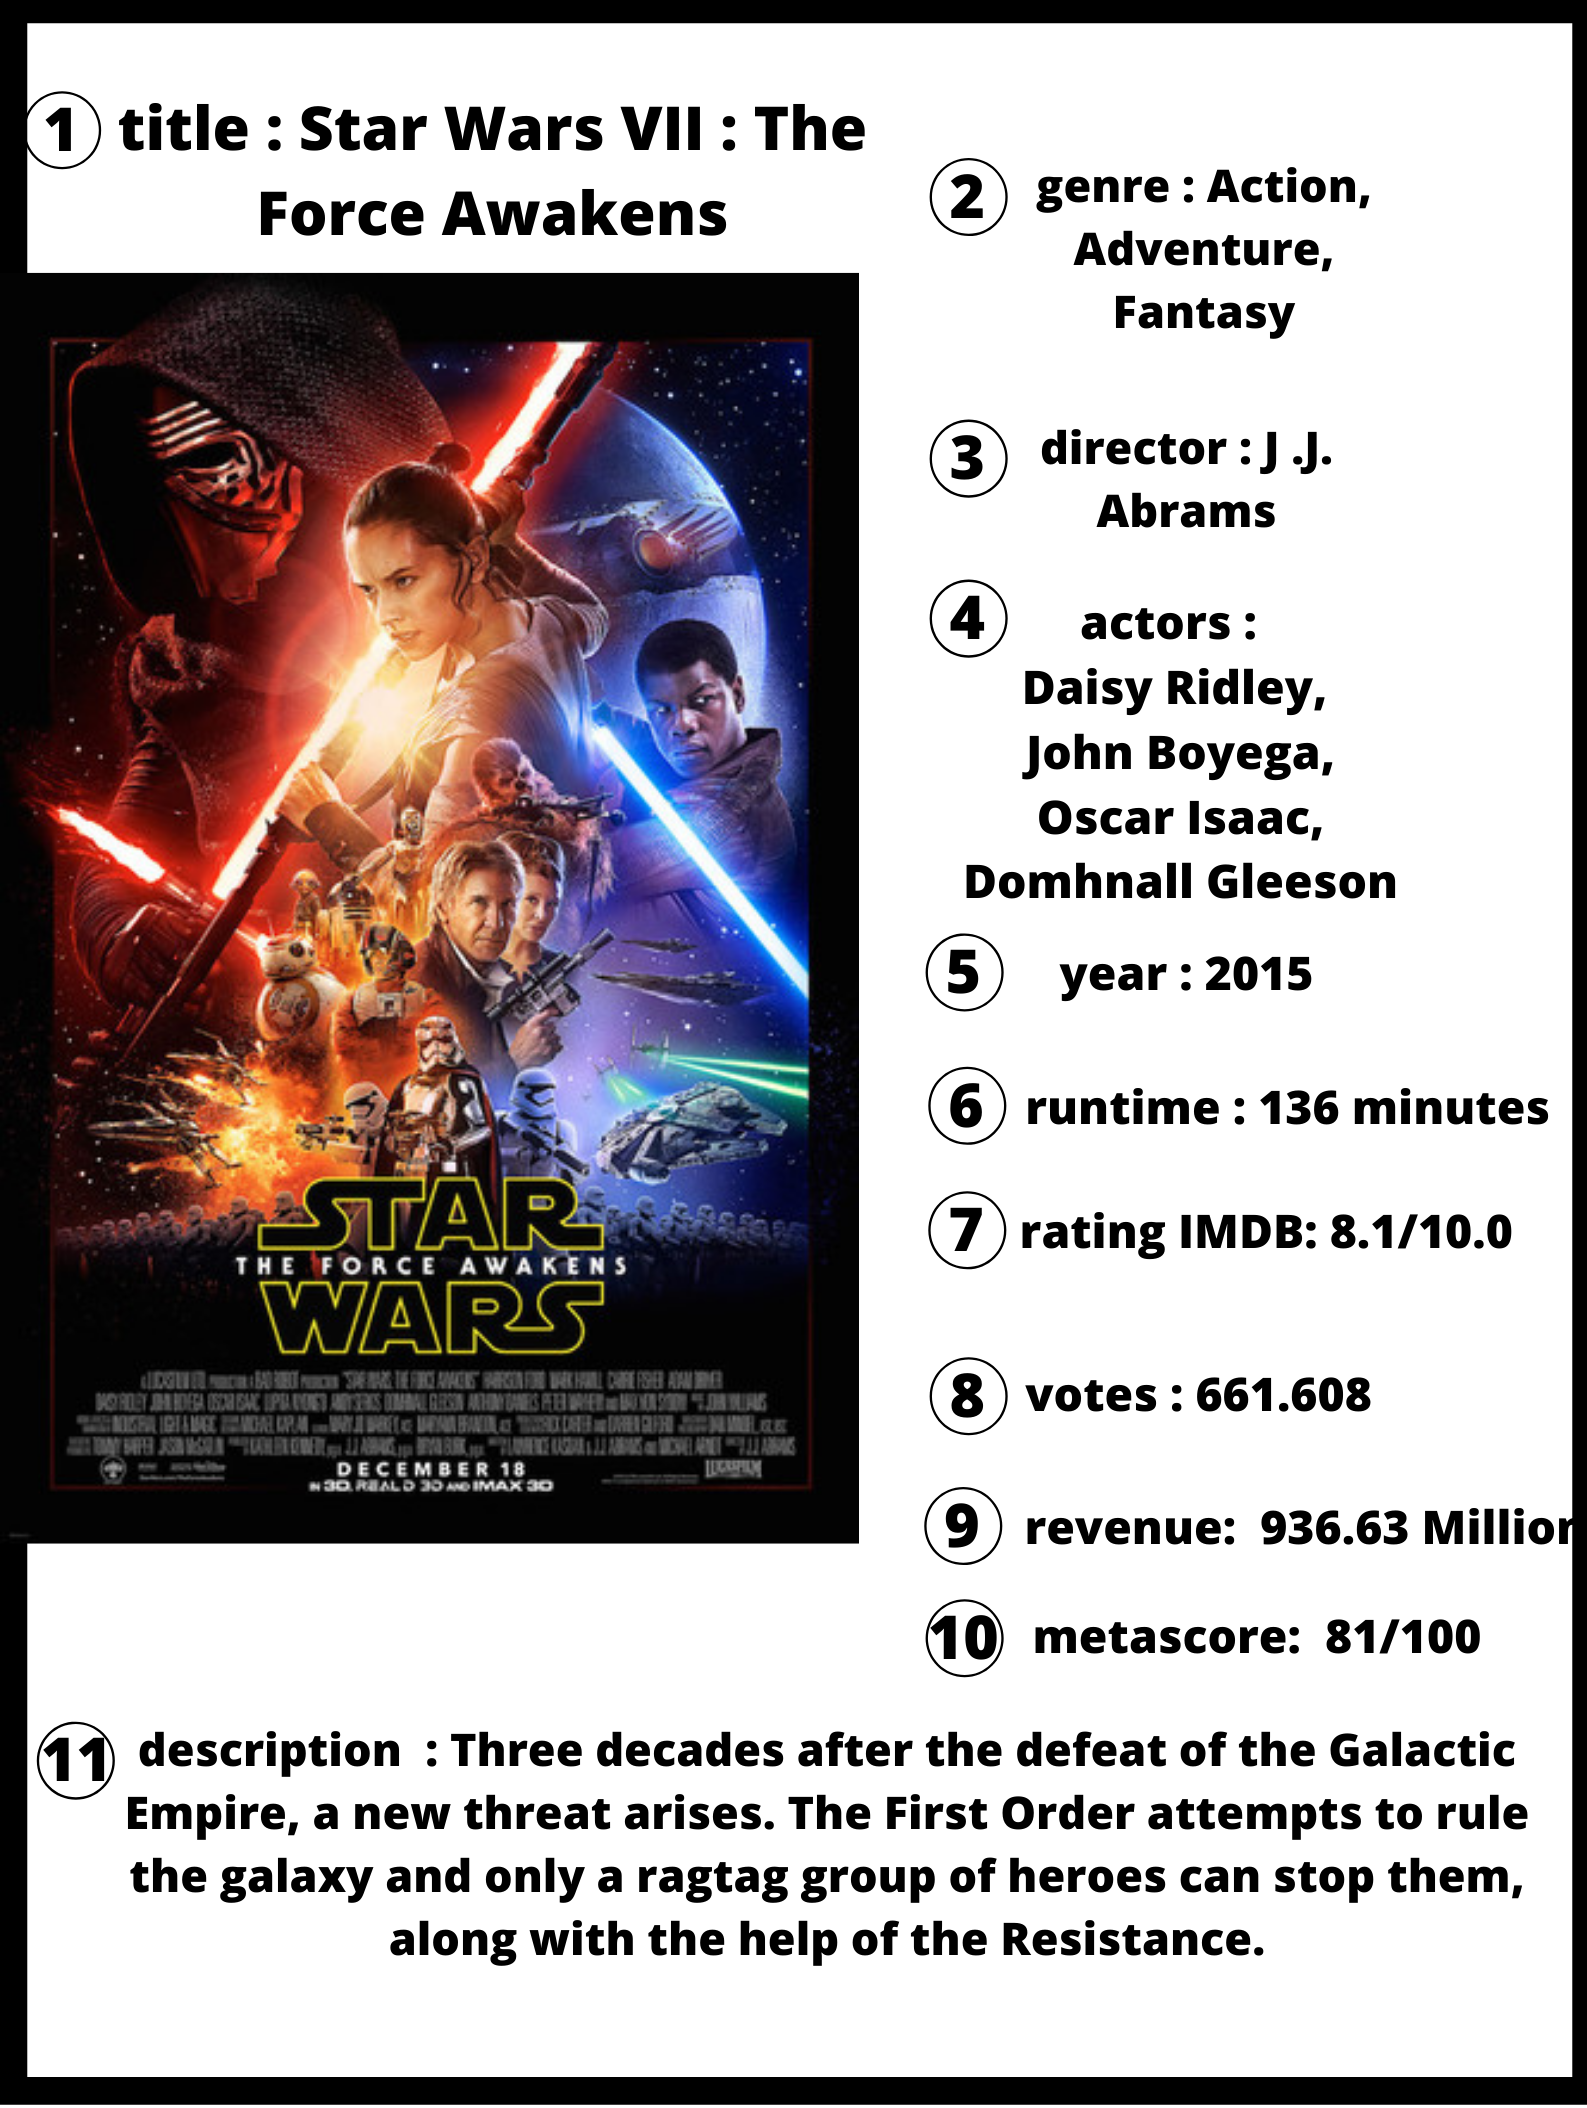
\includegraphics[scale=0.2]{bab4/contohsaturow}   
	\caption{Ilustrasi sebuah baris film pada dataset}
	\label{fig:contohsatudataset} 
\end{figure} 


Berdasarkan deskripsi utama dan Gambar \ref{fig:contohsatudataset} di atas, sebuah baris pada \textit{dataset} merepresentasikan sebuah film dengan berbagai informasi yang terkait seperti judul, aktor yang terlibat, skor \textit{rating} dan lain-lain. Berikut adalah deskripsi dari masing masing kolom  \textit{dataset} pada Tabel \ref{tab:deskripsidataset}.

\begin{table}[H]
\centering
\caption{Deskripsi dataset}
\resizebox{\textwidth}{!}{%
\begin{tabular}{|c|l|c|}
\hline 
\parbox{1cm}{\textbf{Nama}} & \parbox{6cm}{\textbf{Deskripsi}} & \parbox{1cm}{\textbf{Tipe}}\\ 
\hline 
\parbox{1cm}{Title} &\parbox{6cm}{ Judul film}& String \\ 
\hline 
Genre  &\parbox{6cm}{Jenis film. Sebuah film dapat memiliki  lebih dari 1 genre. Genre ditulis dan dipisah menggunakan tanda koma} & String \\
\hline 
Description & Sinopsis film & String \\
\hline 
Director & Nama sutradara & String \\
\hline
Actor & \parbox{6cm}{Nama pemain-pemain film. Sebuah film dapat  memiliki lebih dari satu aktor. Aktor ditulis terpisah dengan tanda koma } & String \\
\hline
Year &  Tahun rilis film & Int \\
\hline 
Runtime &\parbox{6cm}{Durasi film dalam satuan menit} & Int \\
\hline 
Rating & Skor Review dari situs IMDB & Float \\
\hline 
Votes & Jumlah pengguna situs IMDB yang menyukai sebuah film & Int \\
\hline
Revenue& \parbox{6cm}{Pendapatan Kotor Film. \\ Ditulis dalam satuan juta USD} & Float \\
\hline 
Metascore & \parbox{6cm}{Skor review dari situs Metacritic} & Float \\
\hline 
\end{tabular}}
\label{tab:deskripsidataset}
\end{table}

Untuk memahami bagaimana bentuk \textit{dataset}, berikut adalah 5 baris awal  dari \textit{dataset} pada Tabel \ref{tab:datasethead}



\begin{table}[H]
\caption{5 Contoh Data pada dataset}
\resizebox{\textwidth}{!}{%
\begin{tabular}{|l|l|l|l|l|l|l|l|l|l|l|} 
\hline 
Title & Genre & Description & Director & Actors & Year & Runtime & Rating & Votes & Revenue & Metascore \\
\hline
\parbox{1.5cm}{ Guardians  of the galaxy} & \parbox{1.5cm}{Action, \\ Adventure, \\ Sci-fi} & \parbox{1.5cm}{ A group of inter...} & \parbox{1.5cm}{ James Gunn} & \parbox{2cm}{ Chriss Pratt,Zoe Saldana }& 2014 & 121 & $8.1$ & $757074$ & $333.13$ & 76 \\
\hline
\parbox{1.5cm}{Promet\\-heus} & \parbox{1.5cm}{Adventure \\ ,Mystery, \\Sci-fi} & \parbox{1.5cm}{Following clues ...} & \parbox{1.5cm}{Ridley Scott} & \parbox{1.5cm}{Noomi Rapace, Logan Marshall..} & 2012 & 124  & 7 & 485820 & 126.46 & 65 \\
\hline
\parbox{1.5cm}{Split} & \parbox{1.5cm}{Horror,\\ Thriller} & \parbox{1.5cm}{Three girls ...} & \parbox{1.5cm}{M. Night Shyamalan} & \parbox{1.5cm}{James McAvoy, Anya Taylor...} & 2016 & 117 & 7.3 & 157606 & 138.12 & 62 \\
\hline
\parbox{1.5cm}{Sing} & \parbox{1.5cm}{Animation,\\Comedy,\\Family } & \parbox{1.5cm}{in a city of ...} & \parbox{1.5cm}{Christophe Lourdelet} & \parbox{1.5cm}{Matthew McConaughey, Reese Witherspoon} & 2016 & 108 & 7.2 &  60545 & 270.32 & 59 \\
\hline
\parbox{1.5cm}{Suicide Squad} & \parbox{1.5cm}{Action,\\Adventure,\\Fantasy} & \parbox{1.5cm}{A secret government...} & \parbox{1.5cm}{David Ayer} & \parbox{1.5cm}{Will Smith, Jared Leto} & 2016 & 123 & 6.2 & 393727 & 325.02 & 40 \\ 
\hline
\end{tabular}}
\label{tab:datasethead}
\end{table}


\section{Proses Analisis Data Utama} 
\label{chap:hasilanalisisdatautama}
Pada subbab ini dijelaskan analisis awal yang dilakukan dengan menggunakan \textit{dataset} yang sudah disediakan. Tahap-tahap yang dilakukan selama proses analisis data utama adalah : 

\begin{itemize}
\item Melakukan \textit{Data Cleaning} untuk mengatasi \textit{missing value}
\item Melakukan Analisis Visualisasi untuk menemukan pola menarik 
\item Melakukan \textit{Data Selection}
untuk memilih fitur yang berpengaruh untuk prediksi \textit{revenue}
\item Melakukan percobaan prediksi \textit{revenue} berdasarkan fitur menarik menggunakan regresi
\end{itemize}



Penjelasan secara detail mengenai proses analisis data utama ada pada subbab selanjutnya. Berdasarkan hasil analisis data utama yang dilakukan, informasi yang didapat adalah :

\begin{itemize}
\item \textit{Genre} film yang paling banyak dibuat berdasarkan jumlah film dan besar \textit{revenue} yang diperoleh adalah \textit{Action} dan \textit{Adventure} 
\item Selera penonton (\textit{votes}) dalam menilai film tidak sama selera para kritikus / ahli film (\textit{review})
\item Sebuah film relatif lebih mudah mendapatkan nilai \textit{review} yang bagus dari situs IMDB dibanding situs Metacritic
\item Film bioskop umumnya memiliki durasi film dari 60 menit sampai 180 menit. Film yang paling banyak diproduksi adalah film 100 sampai 120 menit. Ada kecenderungan semakin lama durasi film maka semakin banyak peminat
\item Investasi usaha film dapat menguntungkan karena akumulasi \textit{revenue} dan jumlah film yang dibuat tiap tahunnya selalu meningkat 
\item Nilai \textit{review} yang tinggi pada sebuah film tidak menjamin film tersebut dapat meraih keuntungan yang maksimal
\item Penilaian film pada penonton (votes) jauh lebih berpengaruh dari pada penilaian pada situs \textit{review} untuk menentukan kesuksesan film berdasarkan perbandingan korelasi.
\end{itemize}


Penjelasan secara detail mengenai analisis data utama akan dijelaskan selanjutnya.

\subsection{Data Cleaning} 
Pada proses \textit{data cleaning} dilakukan deteksi baris yang mengandung \textit{Null} dengan menggunakan fungsi \textit{dropna()} dari \textit{library pandas}. \textit{Barchart} \ref{fig:barchartnullvalues} adalah visualisasi kolom dan perbandingan jumlah baris yang memiliki \textit{missing value}.

\begin{figure}[H]
	\centering  
	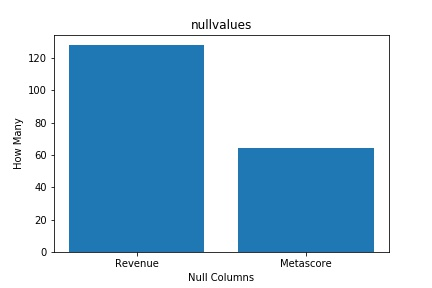
\includegraphics[scale=0.6]{bab4/barchartnullvalues}   
	\caption{Barchart deteksi jumlah baris yang kolomnya terdapat null}
	\label{fig:barchartnullvalues} 
\end{figure} 

Berdasarkan Gambar \ref{fig:barchartnullvalues} di atas, ternyata terdapat baris yang kolom Metascore dan Revenue terdapat \textit{Null}. Baris dengan kolom yang terdapat \textit{Null} dibuang dan tidak diikut sertakan dalam analisis lebih lanjut karena akan menghasilkan \textit{error}. Berdasarkan Gambar \ref{fig:barchartnullvalues}, terdapat 162 baris dengan \textit{null} yang dihilangkan.

\subsection{Analisis Data Utama Menggunakan Visualisasi}
Pada tahap ini dalam proses analisis data utama dilakukan analisis menggunakan visualisasi. Proses visualisasi \textit{dataset} dilakukan untuk menemukan pola menarik.

\subsubsection{Hubungan Genre Dengan Revenue}

Sebuah film dapat memiliki 1 atau lebih \textit{genre}. Fitur \textit{genre} adalah salah satu fitur yang membutuhkan pemrosesan lebih lanjut. Gambar \ref{fig:contohsatudataset} menunjukkan bahwa film \textit Star Wars memiliki lebih dari 1 \textit{genre} yaitu \textit{Action, Adventure }dan \textit{Fantasy}. Untuk menghitung jumlah \textit{genre} untuk setiap film, baris pada \textit{dataset} yang dipisahkan dengan koma harus dipecah menjadi baris yang berbeda.

\begin{table}[H]
\caption{Tabel sebelum \textit{split}}
\centering
\begin{tabular}{|c|c|}
\hline 
title & genre \\ 
\hline 
Star Wars VII : The Force Awakens & Action,Adventure,Fantasy \\ 
\hline 
\end{tabular} 
\label{tab:contohrowsebelumsplit}
\end{table}

\begin{table}[H]
\caption{Tabel setelah \textit{split}}
\centering
\begin{tabular}{|c|c|}
\hline 
title & genre \\ 
\hline 
Star Wars VII : The Force Awakens & Action \\ 
\hline 
Star Wars VII : The Force Awakens & Adventure \\ 
\hline 
Star Wars VII : The Force Awakens & Fantasy \\ 
\hline 
\end{tabular} 
\label{tab:contohrowsetelahsplit}
\end{table}

Ilustrasi Tabel \ref{tab:contohrowsebelumsplit} dan Tabel \ref{tab:contohrowsetelahsplit} menunjukkan teknik untuk memecah \textit{String} pada kolom \textit{genre} yang tergabung dengan \textit{delimiter} koma sehingga menjadi baris yang berbeda. Hasil \textit{genre} yang terpisah sekarang dapat dihitung frekuensi tiap \textit{genrenya}. Visualisasi  frekuensi kemunculan tiap  \textit{genre} untuk semua film pada \textit{dataset} dapat menggunakan \textit{wordcloud}.

\begin{figure}[H]
	\centering  
	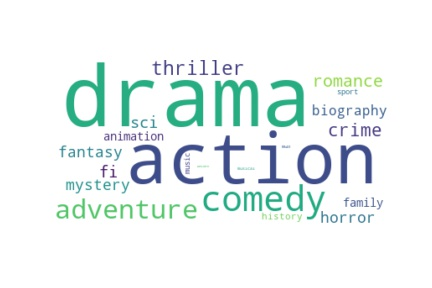
\includegraphics[scale=0.8]{bab4/wordcloud-genre}   
	\caption{Wordcloud kolom genre pada dataset}
	\label{fig:wordcloudgenre} 
\end{figure} 

Gambar \ref{fig:wordcloudgenre} merupakan hasil \textit{wordcloud} dari kolom \textit{genre}. \textit{Wordcloud} adalah visualisasi kemunculan tiap kata yaitu \textit{genre} pada semua \textit{dataset}. Semakin besar huruf suatu kata berarti semakin besar frekuensi kemunculan kata tersebut pada \textit{dataset}. Visualisasi \textit{Piechart} adalah jumlah kemunculan  \textit{genre} tiap film pada \textit{dataset}. 

\begin{figure}[H]
	\centering  
	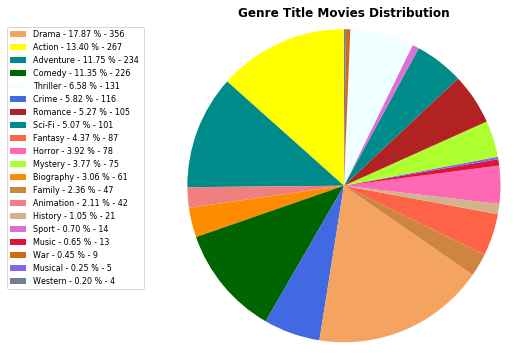
\includegraphics[scale=0.8]{bab4/piechart_genretitle_global}   
	\caption{Piechart persebaran film berdasarkan genre}
	\label{fig:piechart_genretitle_global} 
\end{figure} 

Berdasarkan Gambar \ref{fig:piechart_genretitle_global} di atas, jumlah film yang dibuat terbanyak salah satunya adalah \textit{Drama,Action} dan \textit{Adventure}. Distribusi film berdasarkan \textit{genre} dapat  dijadikan referensi kepada para pembuat film mengenai \textit{genre} apa saja yang sering dibuat.


 Berdasarkan \textit{dataset} yang digunakan, sebuah film memiliki 1 atau lebih \textit{genre}. Visualisasi analisis 10 kombinasi \textit{genre} dengan \textit{revenue} tertinggi dapat menggunakan \textit{boxplot}. \textit{Boxplot} tersebut dapat digunakan untuk membandingkan \textit{revenue} tiap kombinasi \textit{genre} pada \textit{dataset}.


\begin{figure}[H]
	\centering  
	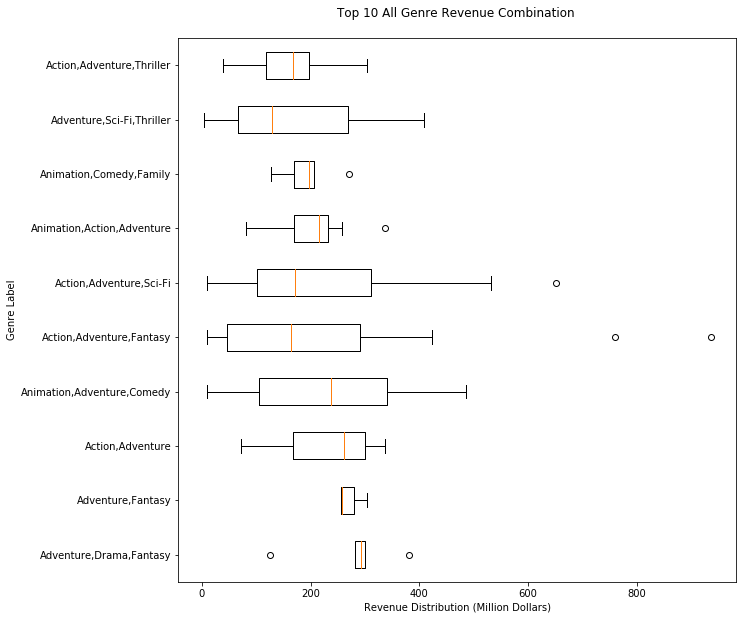
\includegraphics[scale=0.6]{bab4/top10_genre_multiboxplotbyrevenue}   
	\caption{Top 10 Kombinasi genre dengan pendapatan kotor (Revenue) Terbaik}
	\label{fig:top10_genre_multiboxplotbyrevenue} 
\end{figure} 

Gambar \ref{fig:top10_genre_multiboxplotbyrevenue} di atas menunjukkan 10 kombinasi \textit{genre} yang menghasilkan \textit{revenue} paling banyak. Kombinasi \textit{genre} dengan \textit{revenue} terbaik adalah kombinasi \textit{Adventure,Drama,Fantasy}. Referensi ini dapat dijadikan \textit{feedback} untuk pembuat film dalam menentukan \textit{genre}. Film yang mengandung \textit{genre} \textit{action} dan \textit{adventure} cenderung memperoleh kesuksesan karena dari jumlah yang dibuat dan rentang pendapatan relatif tinggi.

\subsubsection{Hubungan Votes dan Review}
Sebuah film memiliki 2 metrik penilaian berdasarkan siapa yang menilainya yaitu \textit{votes} (selera penonton) dan \textit{review} (selera para kritikus). Pada tahap ini akan dianalisis hubungan \textit{votes} dengan fitur \textit{review} yaitu \textit{metascore} dan \textit{rating}. 

\begin{figure}[H]
    \centering
    \subfloat[votes dan rating]{{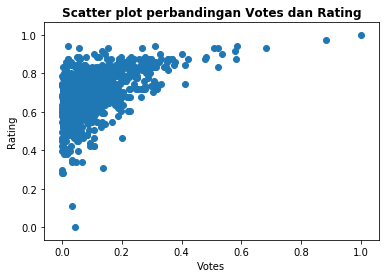
\includegraphics[width=7cm]{bab4/votes_rating_scatterplot} }}%
    \qquad
    \subfloat[votes dan metascore]{{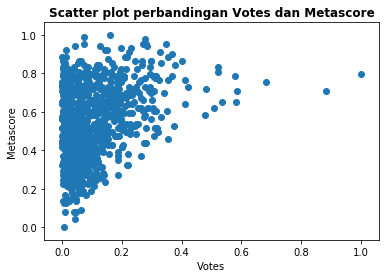
\includegraphics[width=7cm]{bab4/votes_metascore_scatterplot} }}%
    \caption{Hubungan korelasi selera penonton dengan \textit{review}}%
    \label{fig:votes_rating_metascore_scatterplot}%
\end{figure}

Gambar \ref{fig:votes_rating_metascore_scatterplot} adalah visualisasi korelasi antara \textit{votes} dengan \textit{review} menggunakan \textit{scatter plot}. Berdasarkan visualisasi \textit{scatter plot}, \textit{votes} tidak menunjukkan korelasi dengan \textit{rating} maupun \textit{metascore}. Berdasarkan visualisasi yang diberikan, selera penonton pada sebuah film tidak sama dengan selera kritikus.

\subsubsection{Hubungan Metascore Dengan Rating}
Pada tahap ini dilakukan analisis hubungan fitur \textit{metascore} dan \textit{rating} sebagai salah satu metrik penilaian kualitas sebuah film. 

\begin{figure}[H]
	\centering  
	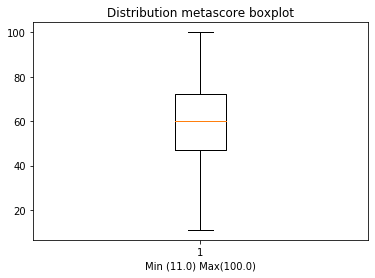
\includegraphics[scale=0.8]{bab4/metascore_boxplot}   
	\caption{Distribusi nilai kolom metascore}
	\label{fig:metascore_boxplot} 
\end{figure} 

Gambar \ref{fig:metascore_boxplot} di atas merupakan distribusi nilai dari \textit{metascore} dengan menggunakan \textit{boxplot}. Nilai minimum dari distribusi \textit{metascore} adalah 11 sehingga terdapat film yang bisa mendapatkan nilai sangat kecil. Perbandingan nilai \textit{metascore} akan dibandingkan dengan nilai \textit{rating}.

\begin{figure}[H]
	\centering  
	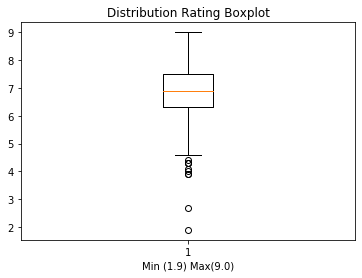
\includegraphics[scale=0.8]{bab4/rating_boxplot}   
	\caption{Distribusi nilai kolom rating}
	\label{fig:rating_boxplot} 
\end{figure} 

Gambar \ref{fig:rating_boxplot} di atas merupakan distribusi nilai dari \textit{rating} menggunakan \textit{boxplot}. Nilai minimum adalah $1.9$ dan maksimum dari distribusi \textit{rating} adalah $9.0$. Pada tahap ini dilakukan perbandingan
\textit{metascore} dan \textit{rating} \textit{boxplot} yang sudah dinormalisasi. 


\begin{figure}[H]
	\centering  
	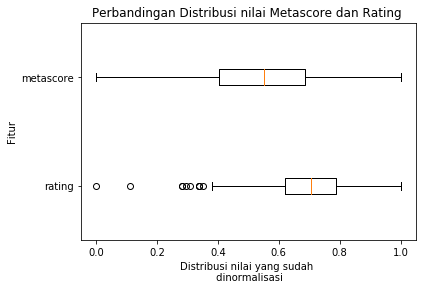
\includegraphics[scale=0.8]{bab4/perbandingan_metascore_rating_boxplot}   
	\caption{Perbandingan Distribusi nilai kolom review}
	\label{fig:perbandingan_metascore_rating_boxplot} 
\end{figure} 

Gambar \ref{fig:perbandingan_metascore_rating_boxplot} adalah perbandingan rentang nilai \textit{boxplot} \textit{metascore} dan \textit{rating} yang sudah dinormalisasi. Nilai Q2 pada \textit{boxplot rating} dan \textit{boxplot metascore} menunjukkan bahwa sebuah film dapat lebih mudah memperoleh nilai lebih baik dengan rating dibanding \textit{metascore}.

\begin{figure}[H]
    \centering
    \subfloat[metascore]{{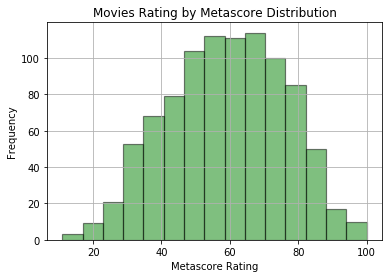
\includegraphics[width=5cm]{bab4/metascore_histogram} }}%
    \qquad
    \subfloat[rating]{{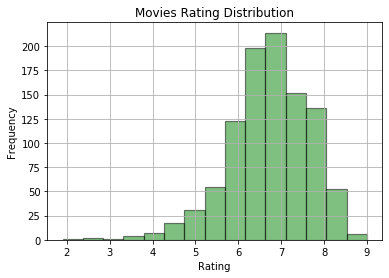
\includegraphics[width=5cm]{bab4/rating_histogram} }}%
    \caption{Histogram kolom metascore dan rating}%
    \label{fig:metascore_ratinghistogram}%
\end{figure}


Gambar \ref{fig:metascore_ratinghistogram} merupakan distribusi nilai \textit{review} pada situs yang berbeda menggunakan \textit{histogram}. Kolom \textit{rating} merupakan nilai \textit{review} dari sumber asal \textit{dataset} yaitu situs IMDB \footnote{https://www.imdb.com/}. Kolom \textit{metascore} adalah nilai \textit{review} yang diberikan oleh situs \textit{review} film yang lain yaitu Metacritic \footnote{https://www.metacritic.com/}. Sebuah film cenderung mendapatkan \textit{review} yang bagus di situs IMDB dibanding situs \textit{metacritic}.

\subsubsection{Hubungan Runtime Dengan Votes}
\begin{figure}[H]
	\centering  
	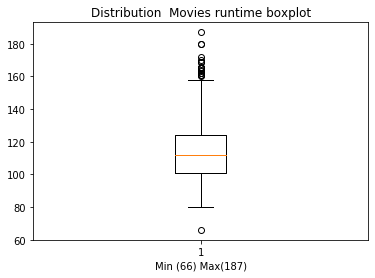
\includegraphics[scale=0.8]{bab4/runtime_boxplot}   
	\caption{Distribusi nilai kolom runtime}
	\label{fig:runtime_boxplot} 
\end{figure} 

Gambar \ref{fig:runtime_boxplot} di atas merupakan distribusi nilai dari \textit{runtime} menggunakan \textit{boxplot}. \textit{Boxplot}  ini dapat membantu pembuat film untuk melihat \textit{range} untuk membuat film dari rentang minimum yaitu sekitar 60 menit hingga 180 menit. Pada tahap selanjutnya dilihat persebaran frekuensi \textit{runtime} menggunakan \textit{histogram}.

\begin{figure}[H]
	\centering  
	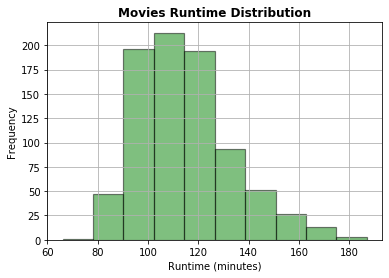
\includegraphics[scale=0.8]{bab4/runtime_histogram}   
	\caption{Distribusi kelas nilai runtime}
	\label{fig:runtime_histogram} 
\end{figure} 

Berdasarkan Gambar \ref{fig:runtime_histogram}, distribusi \textit{runtime} memiliki distribusi normal. Mayoritas film dibuat dengan memiliki durasi 100-120 menit. Pada tahap ini ingin diketahui apakah durasi film yang dibuat sudah memenuhi minat penonton. 

\begin{figure}[H]
	\centering  
	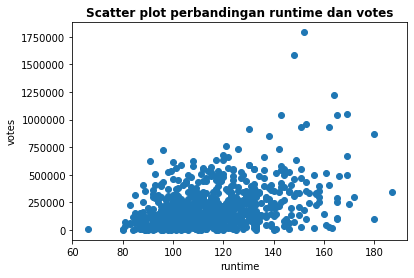
\includegraphics[scale=0.8]{bab4/runtime_votes_scatterplot}   
	\caption{Hubungan korelasi runtime dan votes}
	\label{fig:runtime_votes_scatterplot} 
\end{figure} 

\textit{Scatter plot} pada Gambar \ref{fig:runtime_votes_scatterplot} adalah hubungan korelasi antara durasi film dan jumlah pendukung film pada situs IMDB. Berdasarkan visualisasi yang diberikan, sebuah film cenderung memiliki banyak pendukung jika durasi film semakin lama. Pembuat film dapat memenuhi minat penonton jika pihak pembuat film membuat film dengan durasi yang lebih lama.


\subsubsection{Analisis Votes Dengan Visualisasi}
\begin{figure}[H]
	\centering  
	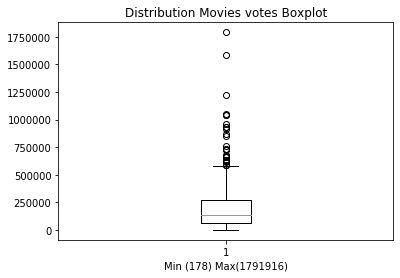
\includegraphics[scale=0.8]{bab4/votes_boxplot}   
	\caption{Distribusi nilai kolom votes}
	\label{fig:votes_boxplot} 
\end{figure} 

Gambar \ref{fig:votes_boxplot} di atas merupakan distribusi nilai dari \textit{votes} menggunakan \textit{boxplot}. Terdapat sebuah film yang memiliki nilai \textit{votes} sangat tinggi. Pada \textit{boxplot} ini, dilakukan deteksi \textit{outlier} dengan cara menghitung \textit{interquartile range} (Q3-Q1). Nilai yang melebihi nilai Q3 + 1.5 * \textit{interquartile range} merupakan \textit{outlier}.


\begin{figure}[H]
	\centering  
	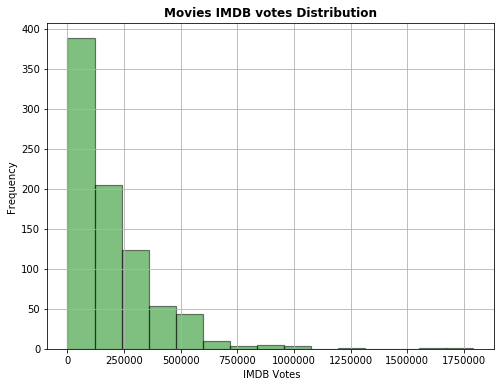
\includegraphics[scale=0.7]{bab4/votes_histogram}   
	\caption{Histogram distribusi kolom votes}
	\label{fig:votes_histogram} 
\end{figure} 

Kolom \textit{votes} merupakan jumlah pengguna situs IMDB yang menyukai sebuah film menggunakan \textit{histogram}. Tiap \textit{bar} merepresentasikan kelompok \textit{range} \textit{votes} yang diperoleh sebuah film. Gambar \ref{fig:votes_histogram} merupakan histogram persebaran \textit{votes} film pada \textit{dataset}. Gambar tersebut menunjukkan bahwa \textit{film} umumnya mendapatkan sampai jumlah $250.000$ \textit{votes}. Film-film yang memiliki \textit{votes} tinggi cenderung merupakan film-film \textit{blockbuster}. Film \textit{blockbuster} adalah sebutan untuk film yang sangat populer dan mendapatkan keuntungan setinggi-tingginya.

\begin{table}[H]
\caption{Film \textit{outlier} berdasarkan \textit{votes}}
\centering
\begin{tabular}{|c|c|c|c|c|c|}
\hline 
Title & Rating & Runtime & Metascore & Revenue & Votes \\ 
\hline 
The Dark Knight & 9 & 152 & 82 & 533.32 & 1,791,916 \\ 
\hline 
Inception & 8.8 & 148 & 74 & 292.57 & 1,583,625 \\ 
\hline 
The Dark Knight Rises & 8.5 & 164 & 78 & 484.13 & 1,222,645 \\ 
\hline 
Interstellar  & 8.6 & 169 & 74 & 187.99 & 1,047,747 \\ 
\hline 
The Avengers & 8.1 & 143 & 69 & 623.28 & 1,045,588 \\ 
\hline 
Django Unchained & 8.4 & 165 & 81 & 162.8 & 1,039,115 \\ 
\hline 
Inglourious Basterds & 8.3 & 153 & 69 & 120.52 & 959,065 \\ 
\hline 
The Departed & 8.5 & 151 & 85 & 132.37 & 937,414 \\ 
\hline 
Avatar & 7.8 & 162 & 83 & 760.51 & 935,408 \\ 
\hline 
The Prestige & 8.5 & 130 & 66 & 53.08 & 913,152 \\ 
\hline 
The Wolf of Wall Street & 8.2 & 180 & 75 & 116.87 & 865,134 \\ 
\hline 
Shutter Island & 8.1 & 138 & 63 & 127.97 & 855,604 \\ 
\hline 
Guardians of The Galaxy & 8.1 & 121 & 76 & 333.13 & 757,074 \\ 
\hline 
Iron Man & 7.9 & 126 & 79 & 318.3 & 737,719 \\ 
\hline 
The Hunger Games & 7.2 & 142 & 68 & 408 & 735,604 \\ 
\hline 
Up & 8.3 & 96 & 88 & 292.98 & 722,203 \\ 
\hline 
\end{tabular} 
\label{tab:film_votesoutlier}
\end{table}
Tabel \ref{tab:film_votesoutlier} di atas, menunjukkan  film \textit{outlier} dengan \textit{votes} tertinggi. \textit{Film} dengan \textit{votes} tinggi cenderung memiliki keuntungan yang besar yaitu lebih dari 100 juta USD.  Film  \textit{outlier} dengan \textit{votes} terbanyak memiliki keuntungan hingga ratusan juta dollar. Berdasarkan tabel di atas pernyataan pada Gambar \ref{fig:metascore_ratinghistogram} juga terbukti. Nilai \textit{review} yang lebih baik mudah diraih di situs IMDB dibanding situs Metacritic. 


\subsubsection{Tren Revenue Dari Tahun Ke Tahun}
\begin{figure}[H]
	\centering  
	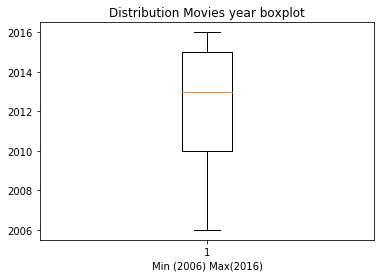
\includegraphics[scale=0.8]{bab4/year_boxplot}   
	\caption{Distribusi nilai kolom year}
	\label{fig:year_boxplot} 
\end{figure} 

Gambar \ref{fig:year_boxplot} merupakan distribusi nilai dari kolom year pada \textit{dataset}. \textit{Boxplot} ini juga dapat digunakan untuk menguji apakah benar \textit{dataset} hanya film yang tahun rilisnya 2006 sampai 2016 sesuai judul dari \textit{dataset} yang digunakan. Selain analisis distribusi dengan \textit{boxplot}, \textit{histogram} juga dapat digunakan untuk melihat distribusi berdasarkan interval nilai kelas. 


\begin{figure}[H]
	\centering  
	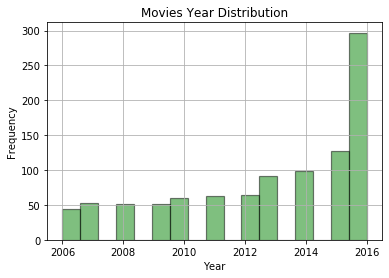
\includegraphics[scale=0.7]{bab4/year_histogram}   
	\caption{Histogram distribusi kolom year }
	\label{fig:year_histogram} 
\end{figure} 

Gambar \ref{fig:year_histogram} merupakan Histogram kolom year. Hasil visualisasi menunjukkan bahwa jumlah film paling banyak dibuat berdasarkan \textit{dataset} ini adalah film yang dibuat pada tahun 2016. Jumlah film yang dibuat dari tahun ke tahun juga meningkat berarti adanya peningkatan minat produksi film sebagai industri hiburan. 


\begin{figure}[H]
	\centering  
	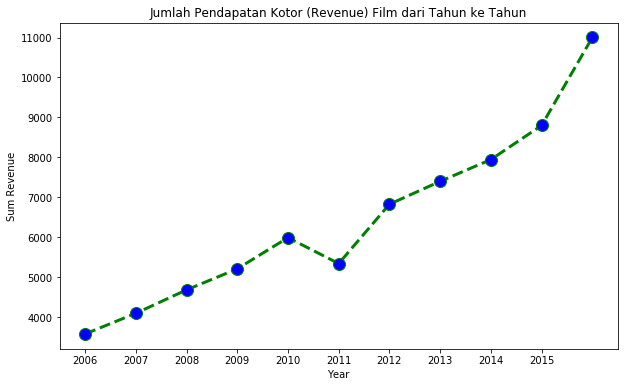
\includegraphics[scale=0.6]{bab4/yearbyyear_revenue_lineplot}   
	\caption{Line plot Jumlah Revenue dari tahun ke tahun}
	\label{fig:yearbyyear_revenue_lineplot} 
\end{figure} 

Gambar \ref{fig:yearbyyear_revenue_lineplot} di atas merupakan visualisasi akumulasi  \textit{revenue} dari tahun ke tahun untuk semua film pada \textit{dataset} menggunakan \textit{line plot}. Berdasarkan visualisasi ini, dapat disimpulkan bahwa dari tahun ke tahun akumulasi \textit{revenue} film semakin meningkat sehingga semaking menguntungkan kecuali pada tahun 2011. Pada tahun 2011 terjadi penurunan akumulasi \textit{revenue}. 

\begin{figure}[H]
    \centering
    \subfloat[Histogram Revenue Tahun 2010]{{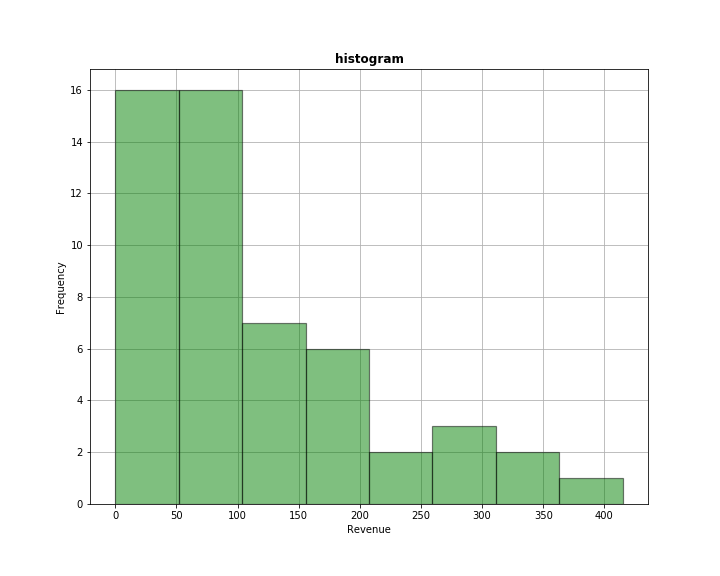
\includegraphics[width=10cm]{bab4/histogram_revenue_2010} }}%
    \qquad
    \subfloat[Histogram Revenue Tahun 2011]{{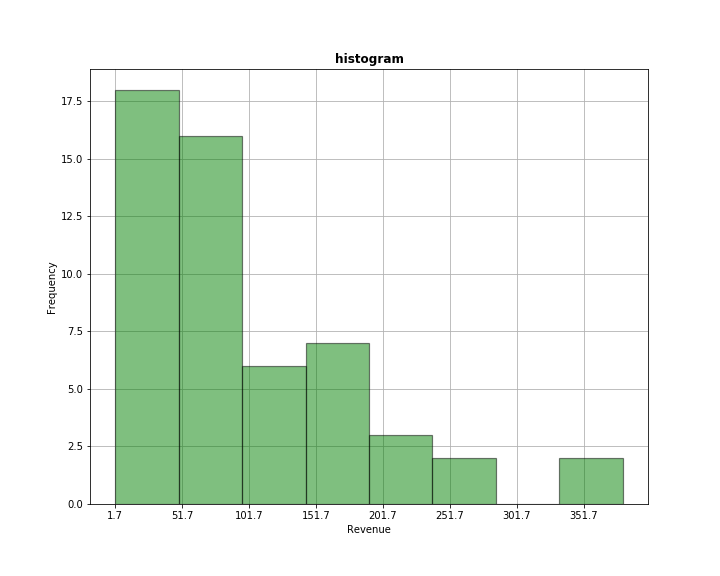
\includegraphics[width=10cm]{bab4/histogram_revenue_2011} }}%
    \caption{Histogram Revenue Tahun 2011}%
    \label{fig:revenue_histogram_2010_2011}%
\end{figure}

Gambar \ref{fig:revenue_histogram_2010_2011} adalah perbandingan distribusi \textit{revenue} film yang dihasilkan pada tahun 2010 dan 2011 menggunakan \textit{histogram}. Berdasarkan visualisasi, tahun 2011 memang mengalami penurunan karena lebih banyak film yang menghasilkan \textit{revenue} kecil dibanding distribusi pada tahun 2010. 



\subsection{Data Selection}
\label{chap:hasildataselection}
Pada subbab ini dilakukan analisis tentang fitur / kolom yang memiliki korelasi dengan \textit{revenue} sebagai penentu kesuksesan sebuah film. Berdasarkan apa yang sudah dijelaskan pada Bab \ref{chap:teori}, visualisasi dengan \textit{scatter plot} dan analisis korelasi numerik \textit{pearson} dapat digunakan untuk menentukan korelasi. Fitur yang memiliki fitur terbaik digunakan sebagai fitur prediktor untuk memprediksi \textit{revenue}. \textit{Dataset} ini memiliki 5 kolom yang menjadi prediktor yaitu \textit{rating, metascore, runtime, year} dan \textit{votes}.  \textit{Revenue} akan menjadi target yang akan diprediksi.

\begin{figure}[H]
    \centering
    \subfloat[Korelasi Metascore dan Revenue]{{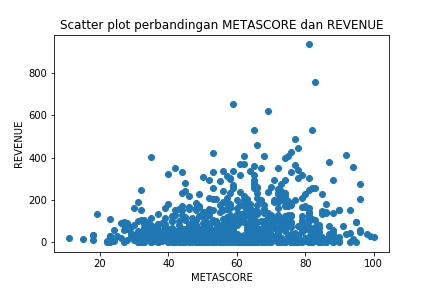
\includegraphics[width=7cm]{bab4/metascore_revenue_scatterplot} }}%
    \qquad
    \subfloat[Korelasi Rating dan Revenue]{{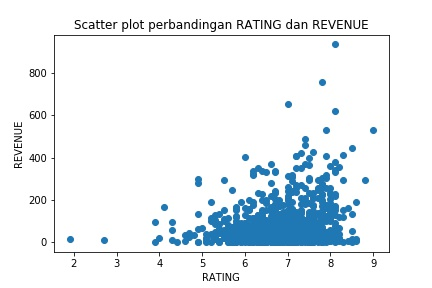
\includegraphics[width=7cm]{bab4/rating_revenue_scatterplot} }}%
    \caption{Analisis Korelasi antara situs review dengan revenue}%
    \label{fig:metascore_rating_revenue_scatterplot}%
\end{figure}


Gambar \ref{fig:metascore_rating_revenue_scatterplot} merupakan \textit{scatter plot} metascore revenue dan rating revenue. Pada gambar tersebut ingin diidentifikasi apakah metascore atau rating mempengaruhi revenue. Berdasarkan gambar yang ditunjukkan rating cenderung lebih memiliki korelasi positif dengan revenue.


\begin{figure}[H]
    \centering
    \subfloat[Korelasi Year dan Revenue]{{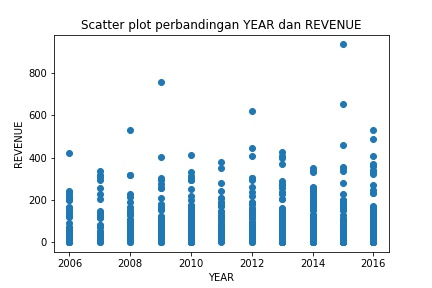
\includegraphics[width=7cm]{bab4/year_revenue_scatterplot} }}%
    \qquad
    \subfloat[Korelasi Runtime dan Revenue]{{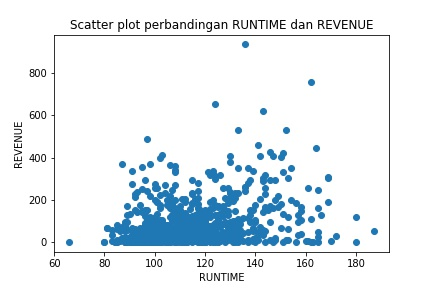
\includegraphics[width=7cm]{bab4/runtime_revenue_scatterplot} }}%
    \caption{Analisis Korelasi runtime year dan  revenue}%
    \label{fig:year_runtime_revenue_scatterplot}%
\end{figure}

Gambar \ref{fig:year_runtime_revenue_scatterplot} merupakan \textit{scatter plot} yang menunjukkan hubungan antara \textit{year revenue} dan \textit{runtime revenue}. Terlihat jelas bahwa \textit{year} tidak ada pengaruh sama sekali terhadap \textit{revenue}. Semakin baru film dirilis tidak menjamin film itu akan sukses menghasilkan keuntungan. Hubungan antara \textit{runtime} dan \textit{revenue} tidak menunjukkan adanya korelasi yang kuat. Durasi film tidak mempengaruhi seberapa bagus film.


\begin{figure}[H]
	\centering  
	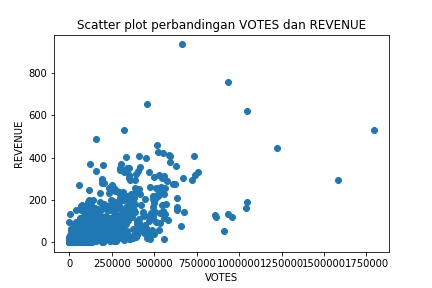
\includegraphics[scale=0.8]{bab4/votes_revenue_scatterplot}   
	\caption{Scatter plot votes dan revenue}
	\label{fig:votes_revenue_scatterplot} 
\end{figure} 


Selain \textit{ runtime, year, rating} dan \textit{metascore}, \textit{votes} adalah salah satu kolom numerik yang dapat dianalisis hubungan korelasinya dengan  \textit{revenue}. Gambar \ref{fig:votes_revenue_scatterplot} adalah visualisasi \textit{scatter plot} votes dan revenue. Hasil visualisasi menunjukkan bahwa votes memiliki korelasi positif dengan revenue. Semakin banyak votes yang diperoleh sebuah film di situs \textit{review} IMDB, maka semakin tinggi kemungkinan film itu akan memperoleh keuntungan. 

Selain visualisasi menggunakan \textit{scatter plot}, pengujian \textit{pearson correlation} berdasarkan subbab \ref{chap:dataselection} dapat digunakan untuk mengukur korelasi antara 2 fitur. 



\begin{figure}[H]
	\centering  
	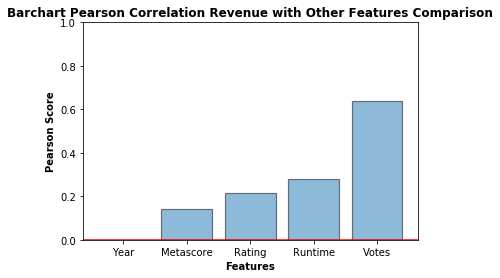
\includegraphics[scale=0.8]{bab4/pearson_iterasi1_revenue_barchart}   
	\caption{Pengujian perbandingan korelasi tiap fitur dengan revenue menggunakan pearson correlation}
	\label{fig:pearson_iterasi1_revenue_barchart} 
\end{figure} 

Gambar \ref{fig:pearson_iterasi1_revenue_barchart} merupakan \textit{barchart} perbandingan nilai \textit{pearson revenue} dengan fitur lain. Gambar tersebut menunjukkan bahwa dari semua fitur numerik, \textit{votes} memiliki korelasi yang paling tinggi. Nilai \textit{pearson} dari votes dan revenue adalah $0.6$. \textit{Pearson} runtime dan revenue adalah $0.3$. \textit{Pearson} rating dan revenue adalah $0.2$. \textit{Pearson} metascore dan revenue adalah $0.1$. Dapat disimpulkan \textit{votes} dapat mempengaruhi revenue yaitu pendapatan kotor dari film. 

\subsection{Percobaan Prediksi Fitur Data Utama}
Pada subbab ini dilakukan percobaan membuat model regresi yang dapat memprediksi keuntungan film yaitu revenue. Prediksi regresi menggunakan \textit{Linear Regression} dan \textit{Polynomial Regression}. Berdasarkan subbab \ref{chap:hasildataselection}, fitur yang memiliki korelasi terbaik adalah \textit{votes}. Pada tahap ini dilakukan pengujian prediksi \textit{revenue} menggunakan \textit{votes}.

\subsubsection{Prediksi Linear Regression Data Utama}
\textit{Dataset} yang digunakan dibagi menjadi 2 bagian yaitu \textit{training} dan \textit{test}. \textit{Dataset} dibagi menjadi $80$ persen dan $20$ persen \textit{test}. Untuk semua pengujian, 80 persen data pertama akan dijadikan \textit{train} dan sisanya dijadikan data \textit{test}. Data \textit{training} akan digunakan untuk menghasilkan fungsi prediksi dari regresi. Fungsi regresi yang dihasilkan akan digunakan untuk prediksi pada data \textit{test} sehingga akurasi / skor R2 dapat diperoleh. 

Berdasarkan hasil data \textit{training}, fungsi prediksi \textit{revenue} adalah 

\begin{equation}
revenueLinearRegression = 15.093793130383503 + 0.00036708749219229494(Votes)
\label{eqref:fungsiLinearIterasi1}
\end{equation}

Persamaan \ref{eqref:fungsiLinearIterasi1} adalah fungsi yang dihasilkan dari regresi menggunakan \textit{Linear Regression}. Fungsi pengujian ini dapat digunakan untuk melakukan percobaan prediksi pendapatan kotor/ revenue. Berikut adalah contoh 5 data film yang diambil dari data \textit{test} dan hasil prediksinya menggunakan fungsi \textit{Linear Regression}.


\begin{table}[H]
\caption{Tabel Percobaan Regresi Linear untuk prediksi revenue menggunakan votes}
\centering
\begin{tabular}{|c|c|c|c|}
\hline 
Title &Votes & Revenue Asli Dataset & Revenue Hasil Prediksi Linear \\ 
\hline 
300:Rise of Empire & 237887 & 106.37 & 102.4191 \\ 
\hline 
Casino Royale & 495106 & 167.01 & 196.841 \\ 
\hline 
True Grit & 254904 & 171.03 & 108.6659 \\ 
\hline 
Norman & 664 & 2.27 & 15.33753923
6 \\ 
\hline 
Self/less& 67196 & 12.28 & 39.7606 \\ 
\hline 
\end{tabular} 
\label{tab:tabel5regresilineariterasi1}
\end{table}


Tabel \ref{tab:tabel5regresilineariterasi1} dapat digunakan untuk melihat perbandingan nilai revenue asli dan hasil prediksi yang dihasilkan oleh \textit{Linear Regression} dengan fitur votes.

\subsubsection{Evaluasi Prediksi Linear Regression Data Utama}
Pengujian prediksi iterasi ini menggunakan 2 dimensi data yaitu prediksi revenue dengan \textit{votes} sehingga visualisasi \textit{Linear Regression} dapat dibuat. Visualisasi dilakukan dengan membuat \textit{scatter plot} dan menarik garis fungsi yang dihasilkan dari \textit{Linear Regression} menggunakan fitur \textit{votes} pada Gambar \ref{fig:linear_regressionplot_votesrevenue}. 

\begin{figure}[H]
	\centering  
	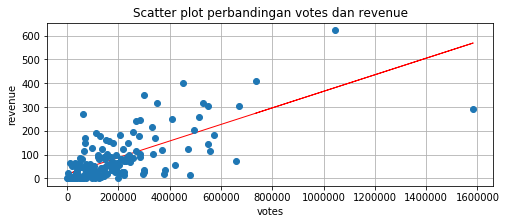
\includegraphics[scale=0.6	]{bab4/linear_regressionplot_votesrevenue}   
	\caption{Plot linear regression prediksi revenue dengan votes}	\label{fig:linear_regressionplot_votesrevenue} 
\end{figure} 

Berikut adalah pengujian evaluasi \textit{Linear Regression} dengan melihat distribusi \textit{squared error} menggunakan \textit{boxplot}. \textit{Squared Error} (SE) adalah ukuran seberapa jauh hasil prediksi dengan nilai asli dari \textit{revenue}. 

\begin{figure}[H]
	\centering  
	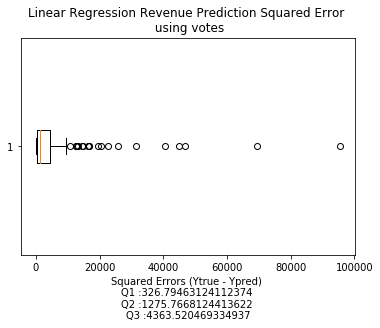
\includegraphics[scale=0.6	]{bab4/squarederror_linear_iterasi1_boxplot}   
	\caption{Distribusi nilai \textit{squared error}}
	\label{fig:squarederror_linear_iterasi1_boxplot} 
\end{figure} 

Gambar \ref{fig:squarederror_linear_iterasi1_boxplot} adalah distribusi nilai \textit{squared error} dari setiap percobaan prediksi pada data \textit{test} menggunakan \textit{boxplot}. Terdapat nilai SE yang sangat tinggi artinya \textit{revenue} asli dan prediksi yang tidak akurat.


\subsubsection{Prediksi Polynomial Regression Data Utama}
Selain \textit{Linear Regression}, percobaan prediksi \textit{revenue} juga dilakukan dengan menggunakan \textit{Polynomial Regression} dengan orde = 2. Hasil kedua algoritma yang digunakan akan dibandingkan performanya dalam melakukan prediksi revenue. Fungsi prediksi revenue menggunakan votes yang dihasilkan \textit{polynomial regression} adalah.

\begin{equation}
revenuePolynomial = 1.162 + 0.000507*(votes) + -1.78E-10*(votes)^2
\label{eqref:fungsipolinomiterasi1}
\end{equation}


Berdasarkan persamaan \ref{eqref:fungsipolinomiterasi1}, akan dilakukan prediksi 5 data \textit{test} dengan fungsi polinom yang dihasilkan. 


\begin{table}[H]
\caption{Tabel Percobaan Regresi Polinom untuk prediksi revenue menggunakan votes}
\centering
\begin{tabular}{|c|c|c|}
\hline 
Votes & Revenue Asli Dataset & Revenue Hasil Prediksi Polinom \\ 
\hline 
237887 & 106.37 & 111.78 \\ 
\hline 
495106 & 167.01 & 208.67 \\ 
\hline 
254904 & 171.03 & 118.92 \\ 
\hline 
664 & 2.27 & 1.50 \\ 
\hline 
67196 & 12.28 & 34.45 \\ 
\hline 
\end{tabular} 
\label{tab:tabelregresi5polinomiterasi1}
\end{table}

Tabel \ref{tab:tabelregresi5polinomiterasi1} di atas adalah tabel perbandingan revenue asli dengan prediksi menggunakan fungsi polinom votes. Terdapat hasil prediksi yang jauh pada \textit{data} ke-2 dan ke-3. 

\subsubsection{Evaluasi Prediksi Polynomial Regression Data Utama}
Karena fungsi polinom dihasilkan dari 2 dimensi menggunakan votes untuk memprediksi revenue, maka visualisasi kurva polinom yang dihasilkan adalah. 



\begin{figure}[H]
	\centering  
	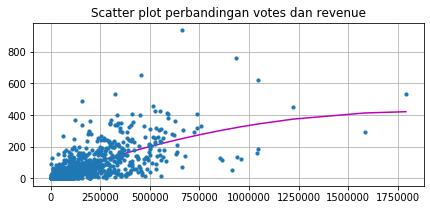
\includegraphics[scale=0.8]{bab4/polynom_regressionplot_votesrevenue}   
	\caption{Plot polynomilal regression prediksi revenue dengan votes}
	\label{fig:polynom_regressionplot_votesrevenue} 
\end{figure} 


Gambar \ref{fig:polynom_regressionplot_votesrevenue} adalah visualisasi kurva yang dihasilkan fungsi polinom menggunakan \textit{scatter plot}. Gambar tersebut dan Gambar \ref{fig:linear_regressionplot_votesrevenue} dapat menunjukkan perbedaan garis yang dihasilkan. Fungsi linear menghasilkan  garis lurus dan fungsi polinom menghasilkan kurva landai. Berikut adalah distribusi nilai \textit{squared error} dari hasil prediksi menggunakan \textit{polynomial regression}. Visualisasi distribusi menggunakan \textit{boxplot}. 



\begin{figure}[H]
	\centering  
	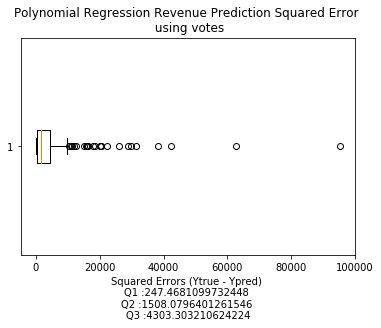
\includegraphics[scale=0.8]{bab4/squarederror_polinomial_iterasi1_boxplot}   
	\caption{Distribusi nilai  squared error prediksi revenue menggunakan \textit{polynomial regression} }
	\label{fig:squarederror_polinomial_iterasi1_boxplot} 
\end{figure} 



\subsubsection{Pengujian Prediksi Data Utama}
Berdasarkan percobaan prediksi dengan fungsi linear dan polinom pada data \textit{test}, akan dilakukan pengujian akurasi nilai ketepatan prediksi menggunakan nilai \textit{coefficient determination} (R2). 

\begin{table}[H]
\caption{Tabel perbandingan skor akurasi r2 menggunakan regresi} 
\centering
\begin{tabular}{|c|c|}
\hline 
Nilai R2 Fungsi Linear & Nilai R2 Fungsi Polinom \\ 
\hline 
 0.38& 0.36  \\ 
\hline 
\end{tabular}

\label{tab:tabelr2_iterasi1}
\end{table}


\begin{figure}[H]
	\centering  
	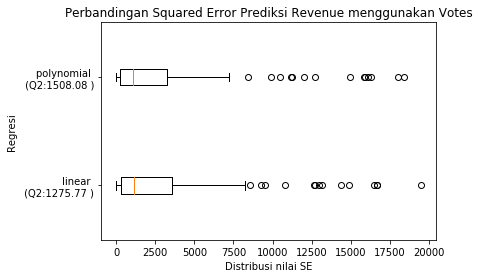
\includegraphics[scale=0.8]{bab4/squarederror_comparison_iterasi1_boxplot}   
	\caption{Distribusi nilai  squared error prediksi revenue dan perbandigan tiap algoritma regresi yang digunakan  }
	\label{fig:squarederror_comparison_iterasi1_boxplot} 
\end{figure} 


Tabel \ref{tab:tabelr2_iterasi1} di atas adalah hasil pengujian skor akurasi fungsi prediksi pada fungsi linear dan polinom. Berdasarkan subbab \ref{chap:evaluasiregresi}, R2 dapat digunakan untuk menguji seberapa baik prediksi yang dihasilkan.  Berdasarkan Gambar \ref{fig:squarederror_comparison_iterasi1_boxplot}, nilai Q2 dari \textit{error} \textit{polynomial} lebih besar dari \textit{linear}. Berdasarkan tabel di atas skor akurasi linear lebih baik dari polinom tetapi, skor yang dihasilkan fungsi linear masih belum tepat untuk melakukan prediksi karena skor yang dihasilkan relatif masih kecil.


\pagebreak


\section{Proses Analisis Data Tambahan}
\label{chap:hasilanalisisdatatambahan}
Berdasarkan informasi kesimpulan yang dihasilkan Subbab \ref{chap:hasilanalisisdatautama} yaitu subbab sebelumnya, model prediksi yang dihasilkan oleh \textit{Linear Regression} dan \textit{Polynomial Regression} masih belum tepat untuk dijadikan model prediksi karena skor akurasi yang kecil yaitu  $0.38$. Hasil analisis \textit{revenue} yang dilakukan juga masih kurang dikarenakan mengukur kesuksesan dengan \textit{revenue} tidak cukup. Analisis \textit{revenue} secara keseluruhan tidak dapat diterapkan karena sebuah film masih memiliki faktor penentu lain yang dominan yaitu \textit{budget}.

Tahap-tahap yang dilakukan selama proses analisis data tambahan adalah : 
\begin{itemize}
\item Melakukan pengumpulan data kolom tambahan \textit{budget} menggunakan \textit{Octoparse} dan API \textit{library} IMDB
\item Melakukan \textit{Data Integration} untuk menggabungkan \textit{dataset} dengan data tambahan \textit{budget}
\item Melakukan \textit{Data Transformation} untuk membuat kolom \textit{profit} dan \textit{Return of Investment} (ROI) berdasarkan \textit{budget} 
\item Melakukan analisis menggunakan visualisasi untuk menemukan pola menarik dari data tambahan 
\item  Melakukan percobaan prediksi \textit{revenue} dan \textit{profit} berdasarkan fitur menarik menggunakan regresi
\end{itemize}


Penjelasan secara detail mengenai proses analisis data tambahan dapat dilihat pada subbab berikutnya. Berdasarkan hasil analisis data tambahan yang dilakukan, informasi yang didapat adalah :

\begin{itemize}
\item Hasil data yang diperoleh dari \textit{scraping} tidak selalu dalam keadaan bersih / sesuai kebutuhan
\item Sebuah film dapat memperoleh \textit{revenue} yang tinggi tetapi belum tentu menghasilkan keuntungan (\textit{profit})
\item Sebuah film dapat mengalami kerugian jika pengeluaran \textit{budget} yang dikeluarkan lebih besar dari pendapatan yang diperoleh \textit{revenue} 
\item Sekitar 61 persen film dari \textit{dataset} memperoleh keuntungan (\textit{revenue} > \textit{budget}) dan 39 persen memperoleh kerugian (\textit{budget} > \textit{revenue})
\item Akumulasi \textit{budget} dan \textit{profit} meningkat tiap tahunnya
\item \textit{Budget} dan \textit{votes} memiliki korelasi yang tinggi dengan \textit{revenue} sehingga penting untuk membuat film yang sesuai keinginan penonton dan menggunakan \textit{budget} semaksimal mungkin untuk kualitas.
\item Nilai evaluasi R2 prediksi \textit{revenue} meningkat dari  $0.38$ menjadi $0.60$ sehingga model  prediksi \textit{revenue} semakin membaik 
\item Nilai evaluasi R2 prediksi \textit{profit} sangat kecil yaitu $0.29$ sehingga tidak dapat digunakan untuk model prediksi. Hal ini disebabkan oleh data film-film yang mengalami kerugian (\textit{profit} negatif) sehingga korelasi semakin melemah 
 \item Film \textit{genre} \textit{Horror/Mystery/Thriller} adalah \textit{genre} film yang dapat menguntungkan walaupun dengan \textit{budget} yang kecil 
\item Film \textit{genre} \textit{Animation} adalah film yang sangat \textit{profitable} tetapi membutuhkan \textit{budget} yang besar 
\item Film \textit{Adventure,Fantasy} adalah salah satu kombinasi \textit{genre} terpopuler
\end{itemize}


\subsection{Data Collection} 
Pengumpulan data \textit{budget} pada \textit{dataset} dilakukan dengan 2 cara yaitu menggunakan \textit{Web Scraping tool} yaitu \textit{Octoparse} dan \textit{Library open source} API dari situs IMDB yaitu IMDBpy. 

\subsubsection{Pengumpulan Menggunakan Octoparse}
Berdasarkan penjelasan \ref{chap:analisiswebscraping}, perangkat lunak \textit{tool} \textit{Octoparse} dapat digunakan untuk mengambil data teks pada sebuah \textit{website}. Pada proses pengumpulan data ini dilakukan pengambilan data \textit{budget} untuk setiap film pada \textit{dataset}.  \textit{Octoparse} hanya dapat mengambil data pada halaman tetapi tidak dapat mengambil data film secara spesifik. Melakukan \textit{scraping} pada semua data film di IMDB akan memakan waktu yang sangat lama dan memperlambat proses analisis. Untuk dapat mengatasi masalah yang dijelaskan, akan dimanfaatkan fitur \textit{advanced search} dari situs IMDB. 


\begin{figure}[H]
	\centering  
	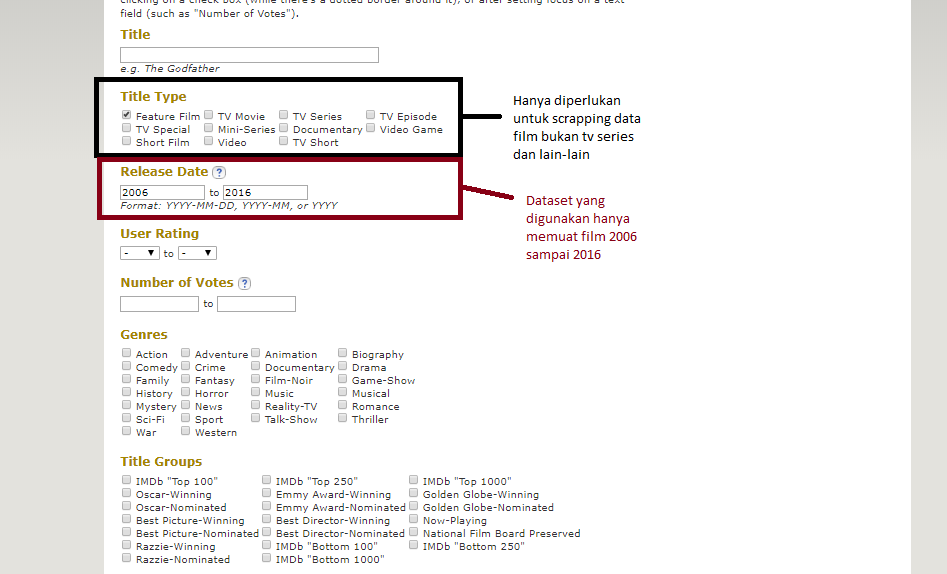
\includegraphics[scale=0.6]{bab4/advancesearchimdb}   
	\caption{Fitur advance search pada situs IMDB}
	\label{fig:advancesearchimdb} 
\end{figure} 


Gambar \ref{fig:advancesearchimdb} adalah fitur \textit{advanced search} pada Situs IMDB. Situs IMDB menuliskan bahwa situs ini memiliki lebih dari 6.5 juta data film. Fitur \textit{advanced search} ini akan membantu proses \textit{scraping} karena hanya akan melakukan \textit{scraping} pada data yang sesuai dengan kriteria \textit{dataset} yang digunakan untuk penelitian. \textit{Dataset} yang diperoleh adalah film terkenal dari tahun 2006 sampai 2016. \textit{Advanced search} pada situs IMDB dapat dimanfaatkan untuk mengambil data khusus sesuai \textit{filter} yang diterapkan sehingga mengurangi waktu untuk melakukan \textit{scraping} pada data yang tidak dibutuhkan.



Hasil dari \textit{advanced search} adalah sebuah hasil \textit{query} dalam bentuk \textit{list}. Sebuah elemen \textit{list} adalah satu objek film beserta data yang dibutuhkan berdasarkan kriteria pencarian pada \textit{advanced search} yang sudah diterapkan. Tipe halaman dengan berisi \textit{list} ini yang dapat dimanfaatkan \textit{Octoparse} agar dapat mengambil data yang dibutuhkan. 

  
\begin{figure}[H]
	\centering  
	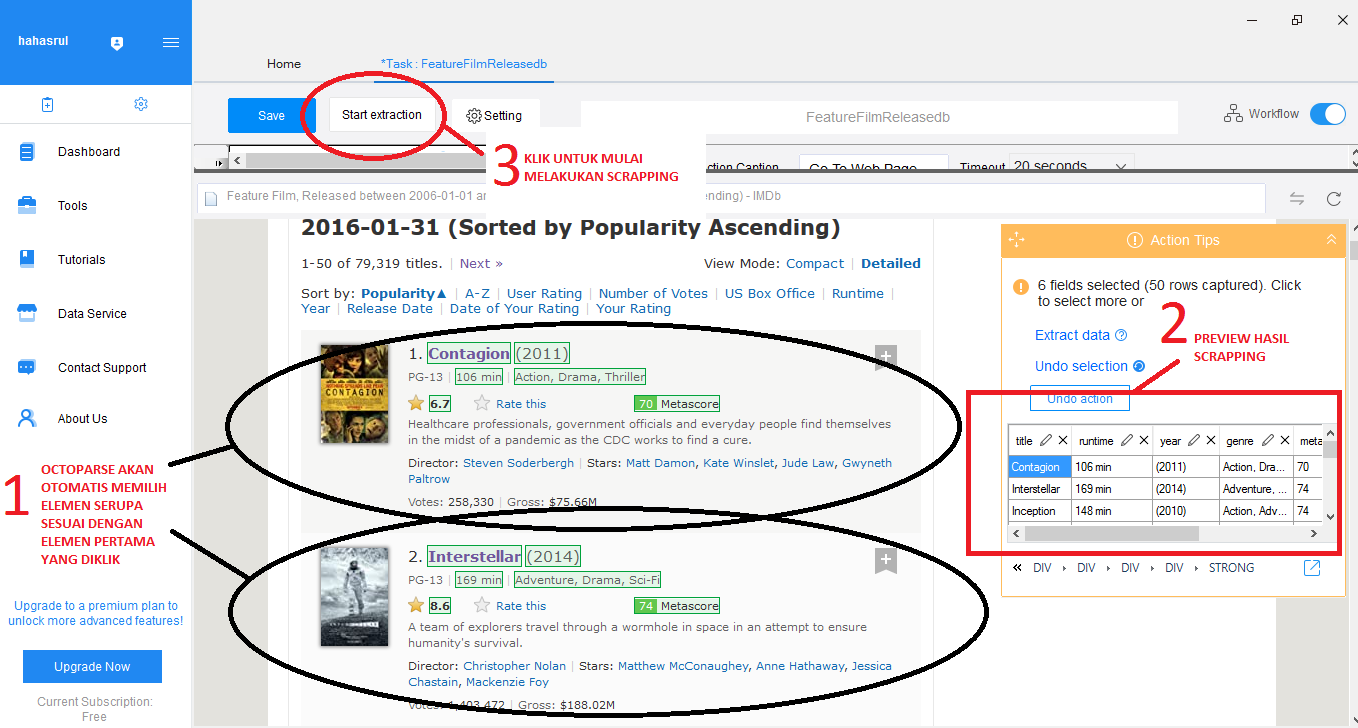
\includegraphics[scale=0.5]{bab4/listelementscrapimdb_octoparse}   
	\caption{Pengaturan octoparse pada hasil pencarian advanced search }
	\label{fig:listelementscrapimdb_octoparse} 
\end{figure} 

Gambar \ref{fig:listelementscrapimdb_octoparse} adalah tampilan pengaturan \textit{Octoparse} untuk melakukan \textit{scraping} pada data IMDB \textit{Octoparse} secara otomatis memberikan rekomendasi untuk elemen yang serupa (film urutan ke-2). Elemen pada \textit{list} merupakan elemen \textit{clickable} yang dapat ditekan \textit{user} untuk masuk halaman  detail sebuah film. \textit{List} tersebut harus diklik untuk dapat mengakses data yang lebih detail yaitu \textit{budget}.

\begin{figure}[H]
	\centering  
	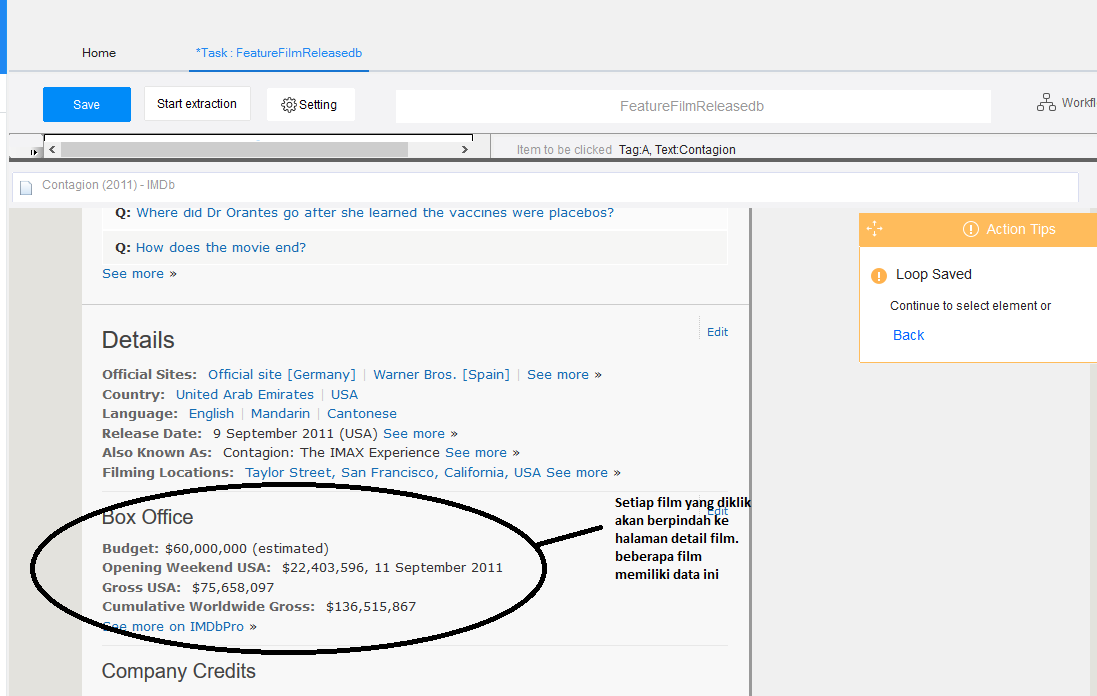
\includegraphics[scale=0.5]{bab4/detailelementscrapingimdb_octoparse}   
	\caption{Detail page sebuah film pada situs IMDB}
	\label{fig:detailelementscrapingimdb_octoparse} 
\end{figure} 

Gambar \ref{fig:detailelementscrapingimdb_octoparse} adalah halaman ketika sebuah film pada gambar sebelumnya diklik. Data \textit{budget} akan tersedia di halaman detail sebuah film. \textit{Flowchart} alur pengambilan data \textit{budget} menggunakan \textit{Octoparse}.

\begin{figure}[H]
	\centering  
	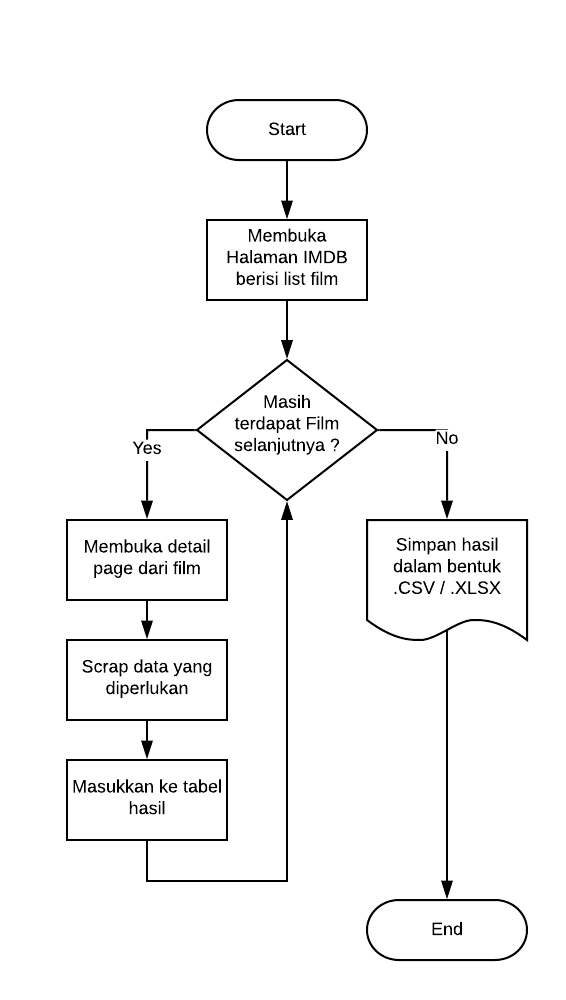
\includegraphics[scale=0.8]{bab4/scrapbudget_imdb_octoparse_flowchart}   
	\caption{Flowchart cara kerja scraping budget IMDB menggunakan Octoparse}
	\label{fig:scrapbudget_imdb_octoparse_flowchart} 
\end{figure} 

Gambar \ref{fig:scrapbudget_imdb_octoparse_flowchart} adalah \textit{flowchart} cara kerja \textit{Octoparse} untuk melakukan \textit{scraping} data tambahan pada situs IMDB. Hasil \textit{scraping} data IMDB menggunakan berjumlah 9337 data film.


\begin{table}
\caption{Sampel contoh data hasil scraping budget IMDB menggunakan Octoparse}
\centering
\begin{tabular}{|c|c|c|c|c|}
\hline 
title & rating & director & budget & runtime \\ 
\hline 
Inception (2010) & 8.8 & Christopher Nolan & Budget: \$160,000,000 & 148 min \\ 
\hline 
The Boy (2016) & 6.0 & William Brent Bell & Budget: \$10,000,000 & 97 min \\ 
\hline 
Sing (2016) & 7.1 & Garth Jennings & Budget: \$ 75,000,000 & 108 min \\ 
\hline 
Moonlight (2016) & 7.4 & Barry Jenkins & Filming Location : Miami & • \\ 
\hline 
\end{tabular} 
\label{tab:hasilscraping_budget_imdb}
\end{table}



Tabel \ref{tab:hasilscraping_budget_imdb} adalah contoh data hasil \textit{scraping} menggunakan \textit{Octoparse}. Terdapat data \textit{budget} yang berhasil diambil dan tidak. Data yang tidak berhasil diperoleh disebabkan karena data \textit{budget} tidak ditampilkan pada halaman sehingga \textit{Octoparse} membaca elemen lain untuk digantikan yaitu \textit{filming location}. Berdasarkan eksperimen pengumpulan data dengan \textit{Octoparse}, data yang diperoleh tidak dapat diintegrasikan ke \textit{dataset} yang dimiliki. Pada tahap selanjutnya dilakukan percobaan pengumpulan data dengan cara lain yaitu mengakses  \textit{open source} API dari IMDB.
 

\subsubsection{Pengumpulan Menggunakan API}
Situs IMDB menyediakan \textit{open source} API yang dapat diakses untuk mengambil data film sesuai kebutuhan. Bahasa pemrograman \textit{Python} membuat \textit{wrapper library} bernama IMDBpy untuk mengakses API dari situs IMDB. \textit{Library} ini memiliki beberapa \textit{method} yang dapat dimanfaatkan :

\begin{itemize}
\item IMDBpy.search\textunderscore movie(title) : \textit{method} untuk melakukan pencarian film dengan parameter \textit{input} \textit{string} judul film. \textit{Method} ini mengembalikan kumpulan objek berisi judul film dan id film tersebut 

\item IMDBpy.get\textunderscore movie(id) : \textit{method} untuk mengambil data film secara lengkap. \textit{Method} ini menerima \textit{input} id dari film yang ingin dicari datanya. \textit{Method} ini mengembalikan sebuah objek film dalam bentuk \textit{dictionary} dengan pasangan \textit{key value} berisi detail data film. \textit{Key} merupakan alamat data yang ingin diambil. \textit{Value} merupakan data yang dihasilkan dari memanggil \textit{key} pada \textit{dictionary}

\item movie.infoset2keys() : \textit{method} untuk melihat kumpulan \textit{key} beserta informasi yang dihasilkan
\end{itemize}

Dengan memanfaatkan \textit{method} yang disediakan IMDBpy, berikut adalah \textit{flowchart} alur kerja pengambilan data \textit{budget} menggunakan \textit{library } IMDBpy

\begin{figure}[H]
	\centering  
	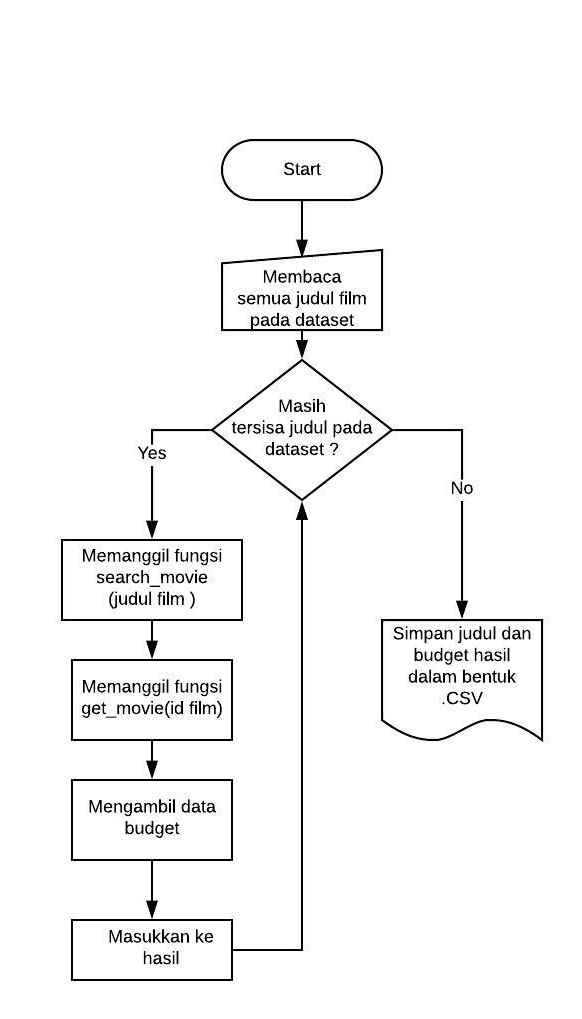
\includegraphics[scale=0.8]{bab4/scrapbudget_imdbpy_api_flowchart}   
	\caption{Flowchart cara kerja scraping budget IMDB menggunakan library IMDBpy}
	\label{fig:scrapbudget_imdbpy_api_flowchart} 
\end{figure} 

Hasil \textit{scraping} dari IMDBpy yang dilakukan adalah sebuah \textit{dataset} dengan kolom judul dan budget dari film tersebut. Jumlah baris dari data tambahan yang diperoleh berjumlah 838 data objek, sesuai dengan jumlah semua film pada \textit{dataset}.

\begin{table}[H]
\caption{Tabel 10 sampel hasil data scrapping menggunakan IMDBpy}
\centering
\begin{tabular}{|c|c|}
  \hline 
  title & budget \\ 
  \hline 
  Guardians of the Galaxy & \$170,000,000 (estimated) \\ 
  \hline 
  Furious 6 & \$160,000,000 (estimated) \\ 
  \hline 
  No Country for Old Men & \$25,000,000 (estimated) \\ 
  \hline 
  The Great Gatsby & \$105,000,000 (estimated) \\ 
  \hline 
  Shutter Island & \$80,000,000 (estimated) \\ 
  \hline 
  Django Unchained & \$100,000,000 (estimated) \\ 
  \hline 
  Busanhaeng & KRW10,000,000 (estimated) \\ 
  \hline 
  The Dressmaker & AUD17,000,000 (estimated) \\ 
  \hline 
  Criminal & 0 \\ 
  \hline 
  The Best of Me & 0 \\ 
  \hline 
  \end{tabular}   
  \label{tab:10sampelhasilscrap_imdbpy_api}
\end{table}

Tabel \ref{tab:10sampelhasilscrap_imdbpy_api} adalah beberapa sampel hasil \textit{scraping} yang dilakukan. Data yang diberikan merupakan estimasi \textit{budget} dari setiap film. Mayoritas film memiliki \textit{budget} dalam mata uang USD. Terdapat beberapa baris yang data \textit{budget} diberikan dalam mata uang selain dollar. Ada beberapa film juga yang memang tidak menyimpan data \textit{budget} sehingga diberikan nilai $0$. Hasil data yang berhasil diperoleh digunakan untuk analisis subbab selanjutnya. 



\subsection{Data Integration}
Data tambahan \textit{budget} yang sudah diperoleh sebelumnya akan digunakan untuk digabungkan dengan \textit{dataset}. Cara penggabungan akan dilakukan dengan operasi \textit{merge}. Tiap baris pada \textit{dataset} dipasangkan dengan baris pada data \textit{budget}. Masing-masing tabel memiliki kolom unik yang serupa yaitu title sehingga title akan dijadikan \textit{key}. 

\begin{table}[H]
\caption{Tabel sampel data integrasi antara dataset dengan budget}
\centering
\begin{tabular}{|c|c|c|}
\hline 
title & genre & budget \\ 
\hline 
Guardians of the Galaxy & Action,Adventure,Sci-Fi
 & \$170,000,000 (estimated) \\ 
\hline 
Prometheus & Adventure,Mystery,Sci-Fi
 & \$130,000,000 (estimated) \\ 
\hline 
Split & Horror,Thriller & \$90,000,000 (estimated) \\ 
\hline 
\end{tabular} 
\label{tab:tabeldataintegrasiiterasi2}
\end{table} 


\subsection{Data Transformation}
Data \textit{budget} yang diperoleh pada subbab sebelumnya adalah data biaya yang dikeluarkan untuk membuat sebuah film. Masing-masing film memiliki \textit{budget} yang bervariasi. Berdasarkan Tabel \ref{tab:tabeldataintegrasiiterasi2}, data \textit{budget} belum bisa dianalisis karena : 

\begin{itemize}
\item Data \textit{budget} masih berbentuk tipe data \textit{string} (contoh : "\$130,000,000")
\item Masih terdapat karakter untuk menentukan mata uang (contoh : "KRW" , "\$" , "EUR")
\item Ada data yang memiliki mata uang yang berbeda
\end{itemize}

Berdasarkan permasalahan \textit{budget} yang dijelaskan sebelumnya, maka dilakukan \textit{data transformation} untuk mengubah data \textit{budget} menjadi bentuk yang lebih sesuai. Kolom \textit{revenue} sebagai pendapatan kotor memiliki tipe \textit{float} dan disimpan dalam satuan juta \textit{dollar} sehingga kolom \textit{budget} perlu diubah menjadi bentuk yang sesuai dengan \textit{revenue}. 

\begin{table}[H]
\caption{Tabel sampel beberapa konversi budget pada dataset}
\centering
\begin{tabular}{|c|c|c|c|c|}
 \hline 
 Title & Budget  & Operasi & Pengali  & Budget \\ 
 Film  & Sebelum & Konversi & Mata Uang & Sesudah \\
 \hline
 Guardians of the Galaxy & \$170,000,000  & - & - & 170 \\ 
 \hline 
 Furious 6  & \$160,000,000  & - & - & 160 \\ 
 \hline 
 Busanhaeng & KRW10,000,000  & KRW -> USD & 0.00082 & 8.2 \\ 
 \hline 
 The Dressmaker & AUD17,000,000 & AUD -> USD & 0.65 & 11.05 \\ 
 \hline 
 ... & ... & ... & ... & ... \\ 
 \hline 
 \end{tabular}  
\label{tab:sampelkonversibudgetpadadataset}
\end{table}

Tabel \ref{tab:sampelkonversibudgetpadadataset} adalah tabel sampel data pada \textit{dataset} yang diubah sesuai format yang serupa dengan \textit{revenue}. Terdapat film yang memiliki mata uang yang berbeda sehingga harus diubah secara manual menggunakan perangkat lunak Microsoft Excel. Setelah semua \textit{budget} sudah diubah dalam bentuk \textit{dollar}, lalu \textit{budget} diubah dalam bentuk satuan juta USD. 

\textit{Dataset} yang digunakan sudah memiliki kolom \textit{budget} yang sesuai untuk dianalisis. Pada tahap selanjutnya dilakukan \textit{data transformation} dengan teknik \textit{attribute construction} sesuai dengan subbab \ref{chap:datatransformation}. \textit{Attribute construction} adalah teknik membuat kolom baru berdasarkan perhitungan kolom yang ada. Pada tahap ini dilakukan dua kali \textit{Attribute construction} untuk membuat kolom pendapatan bersih (profit) dan \textit{return of investment} (ROI).

\begin{equation}
Pendapatan Bersih / Profit = Revenue - Budget
\label{eqref:rumusprofit}
\end{equation} 

Persamaan \ref{eqref:rumusprofit} adalah cara menghitung pendapatan bersih / \textit{profit}. Berikut adalah tabel 5 film sampel pada \textit{dataset} pada Tabel \ref{tab:5sampel_pembuatan_profit}.

\begin{table}[H]
\caption{Tabel 5 sampel pembuatan kolom profit pada  dataset}
\centering
\begin{tabular}{|c|c|c|c|}
  \hline 
  title & revenue & budget & revenue - budget = profit \\ 
  \hline 
  Ted 2 & 81.26 & 68 & 81.26 - 68 = 13.26 \\ 
  \hline 
  The Conjuring 2 & 102.46 & 40 & 102.46 - 40 = 62.46 \\ 
  \hline 
   Toy Story 3  & 414.98 & 200 & 414.98-200 = 214.98 \\ 
  \hline 
  The Skin I Live In & 3.19 & 13 & 3.19 - 13 = (-9.81) \\ 
  \hline 
  Nine Lives & 19.64 & 30 & 19.46 - 40  = (-20.54) \\ 
  \hline 
  \end{tabular}   
\label{tab:5sampel_pembuatan_profit}
\end{table}

Tabel \ref{tab:5sampel_pembuatan_profit} adalah 5 sampel yang diambil dari \textit{dataset} dan perhitungan \textit{profit} tiap datanya untuk menghasilkan kolom baru. Selain kolom \textit{profit}, dilakukan \textit{attribute construction} untuk membuat kolom \textit{Return Of Investment} (ROI). ROI adalah laba di atas pengeluaran. ROI adalah presentase seberapa untung laba berdasarkan perbandingannya dengan pengeluaran / \textit{budget}. Berikut adalah cara menghitung ROI. 

\begin{equation}
ROI = profit / budget * 100
\label{eqref:rumusroi}
\end{equation} 


Persamaan \ref{eqref:rumusroi} adalah rumus yang dapat digunakan untuk memperoleh ROI sebuah film. Berikut adalah 5 sampel contoh perhitungan ROI pada \textit{dataset}.


\begin{table}[H]
\caption{Tabel 5 sampel pembuatan kolom roi pada dataset}
\centering
\begin{tabular}{|c|c|c|c|}
\hline 
title & budget & profit & roi = profit / budget * 100 \\ 
\hline 
Spider-Man 3 & 259 & 78.53 & $\frac{78.53}{259} *100 = 30.43 \% $ \\ 
\hline 
The Intern & 35 & 40.27 & $\frac{40.27}{35}* 100 = 115.06 \% $ \\ 
\hline 
Silver Linings Playbook & 21 & 111.09 & $\frac{111.09}{21}*100 = 529  \% $ \\ 
\hline 
A United Kingdom & 14 & -10.1 & $\frac{-10.1}{14}* 100 = -72.14 \% $ \\ 
\hline 
The Curious Case of Benjamin Button & 150 & -22.51 & $\frac{-22.51}{150} * 100 = -15.01  \%$ \\ 
\hline 
\end{tabular} 
\label{tab:5sampel_pembuatan_roi}
\end{table}

Tabel \ref{tab:5sampel_pembuatan_roi} adalah contoh 5 sampel perhitungan ROI pada \textit{dataset}. Berdasarkan contoh yang diberikan, terdapat film yang memperoleh kerugian bukan keuntungan karena \textit{profit} dan \textit{roi} bernilai negatif. Nilai negatif berarti pengeluaran yang dikeluarkan lebih besar dari keuntungan yang didapat. Pada subbab selanjutnya akan dilakukan analisis visualisasi terhadap \textit{dataset} dengan kolom baru.


\subsection{Analisis Data Tambahan Menggunakan Visualisasi}
Berdasarkan data tambahan yang sudah diperoleh pada subbab sebelumnya, dilakukan visualisasi distribusi nilai kolom tambahan yaitu \textit{budget} , \textit{profit} dan \textit{ROI}.

\begin{figure}[H]
	\centering  
	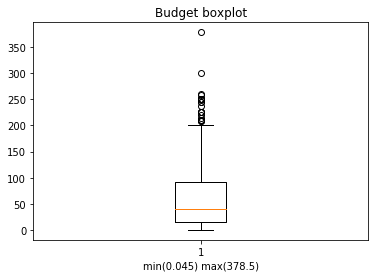
\includegraphics[scale=0.6]{bab4/budget_boxplot}   
	\caption{Distribusi nilai kolom budget}
	\label{fig:budget_boxplot} 
\end{figure} 


Gambar \ref{fig:budget_boxplot} adalah visualisasi distribusi \textit{budget} menggunakan \textit{boxplot}. Visualisasi ini menunjukkan bahwa untuk membuat film dengan modal yang kecil. Nilai minimum \textit{budget} pada \textit{dataset} ini adalah $0.045$. Nilai tersebut ditulis secara satuan juta \textit{dollar} sehingga nilai minimum dari \textit{budget} adalah $45,000$ \textit{dollar}. 

\subsubsection{Hubungan Profit Sebagai Keuntungan}

\begin{figure}[H]
	\centering  
	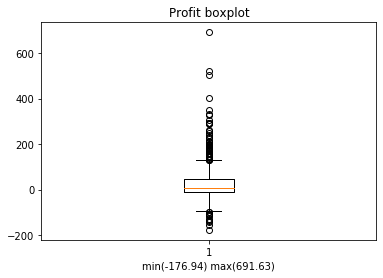
\includegraphics[scale=0.6]{bab4/profit_boxplot}   
	\caption{Distribusi nilai kolom profit}
	\label{fig:profit_boxplot} 
\end{figure} 

Gambar \ref{fig:profit_boxplot} adalah visualisasi distribusi \textit{profit} menggunakan \textit{boxplot}. Berdasarkan \textit{boxplot profit} yang ditunjukkan, usaha film ternyata bisa menyebabkan kerugian ketika modal / \textit{budget} yang dikeluarkan jauh lebih besar dari keuntungan yang diperoleh. Nilai minimum dari \textit{profit} yang dapat diperoleh adalah $-179.94$ juta USD. Berikut adalah perbandingan film yang rugi dan menguntungkan pada Gambar \ref{fig:perbandinganfilm_untungrugi_piechart}

\begin{figure}[H]
	\centering  
	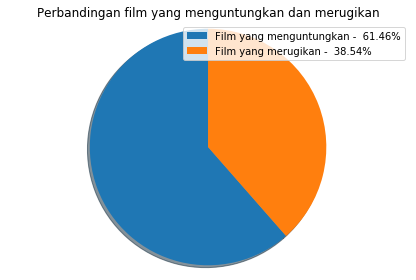
\includegraphics[scale=0.6]{bab4/perbandinganfilm_untungrugi_piechart}   
	\caption{Perbandingan film yang rugi dan untung pada dataset}
	\label{fig:perbandinganfilm_untungrugi_piechart} 
\end{figure} 


\subsubsection{Analisis ROI}

\begin{figure}[H]
	\centering  
	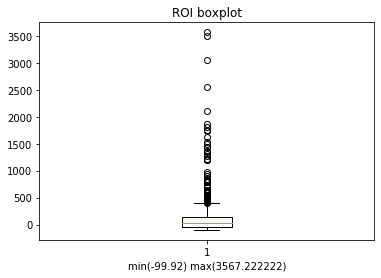
\includegraphics[scale=0.6]{bab4/roi_boxplot}   
	\caption{Distribusi nilai kolom ROI}
	\label{fig:roi_boxplot} 
\end{figure} 


Gambar \ref{fig:roi_boxplot} adalah visualisasi distribusi \textit{roi} \textit{dataset} menggunakan \textit{boxplot}. Berdasarkan \textit{boxplot ROI} yang ditunjukkan, sebuah film bisa aja rugi sampai 2 kali lipat. Dapat dilihat bahwa nilai minimumnya adalah $-99.92$. Artinya sebuah film bisa memperoleh kerugian sampai 99 persen tetapi, ada film yang bisa memperoleh keuntungan sampai jauh lebih tinggi sampai lebih dari 100 persen. Selain visualisasi dengan \textit{boxplot}, maka diberikan visualisasi distribusi menggunakan \textit{histogram}.


\subsubsection{Analisis Histogram}

\begin{figure}[H]
	\centering  
	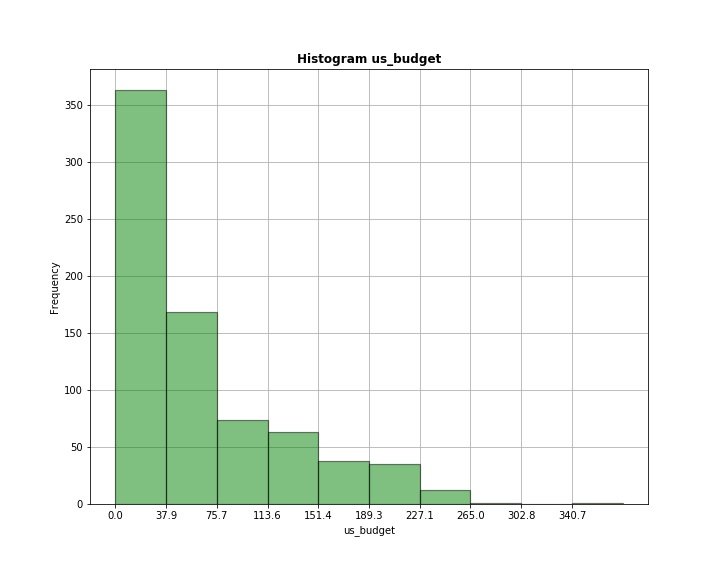
\includegraphics[scale=0.5]{bab4/budget_histogram}   
	\caption{Histogram kolom Budget}
	\label{fig:budget_histogram} 
\end{figure} 



\begin{figure}[H]
	\centering  
	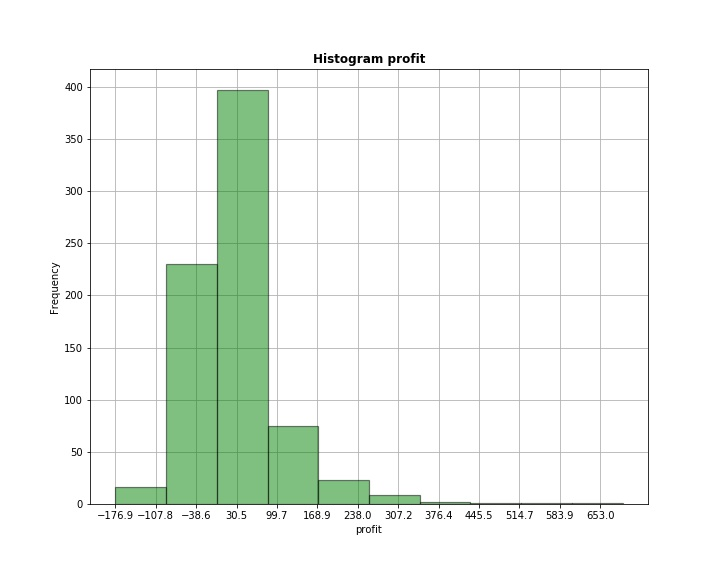
\includegraphics[scale=0.5]{bab4/profit_histogram}   
	\caption{Histogram kolom Profit}
	\label{fig:profit_histogram} 
\end{figure} 

Gambar \ref{fig:budget_histogram} dan \ref{fig:profit_histogram} adalah perbandingan \textit{histogram} \textit{budget} dengan \textit{profit}. Hasil visualisasi dapat menunjukkan bahwa umumnya sebuah banyak film yang menghabiskan \textit{budget} pada kelompok $0$ sampai $30$ juta \textit{dollar}. Selain itu, visualisasi \textit{histogram profit} menunjukkan bahwa banyak film dapat memperoleh  sekitar $90$ juta \textit{dollar}. 


\begin{figure}[H]
	\centering  
	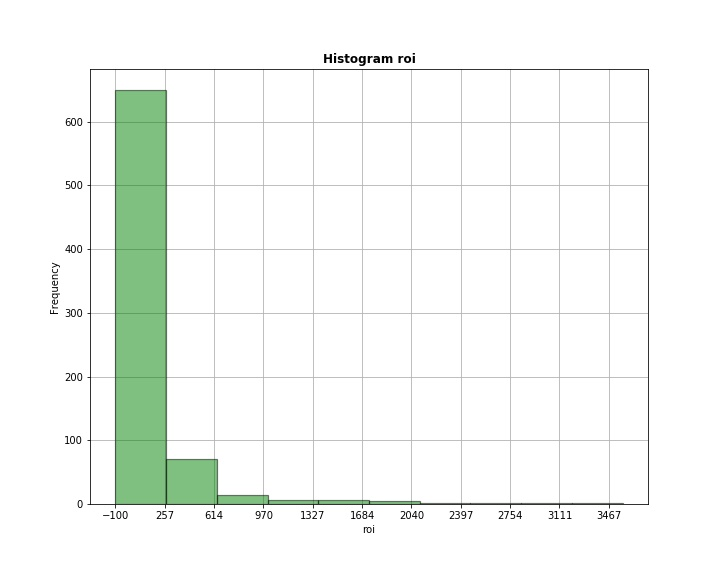
\includegraphics[scale=0.5]{bab4/roi_histogram}   
	\caption{Histogram kolom ROI}
	\label{fig:roi_histogram} 
\end{figure} 

Gambar \ref{fig:roi_boxplot} adalah persebaran frekuensi kelompok ROI pada \textit{dataset}. Berdasarkan persebaran distribusinya mayoritas dari film pada \textit{dataset} memperoleh dari $-100\%$ sampai $200\%$. Sebuah film bisa saja rugi atau memperoleh keuntungan sampai 2 kali lipat. Pada tahap ini dilakukan analisis akumulasi \textit{budget} dan \textit{profit} film dari tahun ke tahun.

\subsubsection{Tren Budget Dan Profit Dari Tahun ke Tahun}
\begin{figure}[H]
	\centering  
	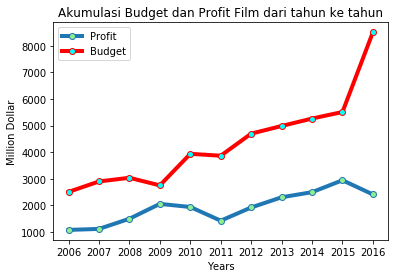
\includegraphics[scale=0.6]{bab4/yearbyyear_budgetprofit_lineplot}   
	\caption{Line plot akumulasi profit dan budget semua film tiap tahun}
	\label{fig:yearbyyear_budgetprofit_lineplot} 
\end{figure} 

Gambar \ref{fig:yearbyyear_budgetprofit_lineplot} adalah analisis akumulasi \textit{budget} dan \textit{profit} dari tahun ke tahun menggunakan \textit{line plot}. Berdasarkan visualisasi dapat disimpulkan bahwa \textit{profit} keuntungan dari membuat film tiap tahun meningkat. \textit{Profit} meningkat seiring dengan \textit{budget} yang harus dikeluarkan. Ada peningkatan signifikan dari tahun 2015 ke tahun 2016. Hal ini disebabkan oleh data film yang rilis tahun 2016 jauh lebih banyak dari data film selain 2016 pada \textit{dataset}.    

Berdasarkan kesimpulan pada subbab \ref{chap:hasilanalisisdatautama} pada bagian \textit{data selection}, kolom \textit{votes} adalah kolom yang memiliki korelasi positif paling tinggi terhadap keuntungan yaitu \textit{revenue}. Pada tahap ini dilakukan analisis distribusi \textit{votes} yang diperoleh tiap kombinasi \textit{genre} film. Berikut adalah visualisasi 10 kombinasi \textit{genre} yang memiliki distribusi \textit{votes} yang paling besar menggunakan \textit{boxplot}. 


\begin{figure}[H]
	\centering  
	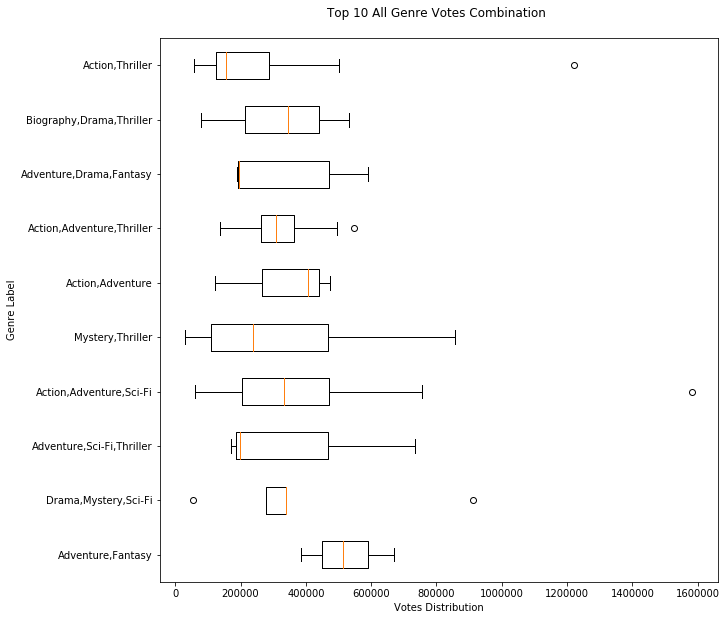
\includegraphics[scale=0.6]{bab4/top10_genre_multiboxplotbyvotes}   
	\caption{Top 10 Kombinasi genre dengan votes terbaik}
	\label{fig:top10_genre_multiboxplotbyvotes} 
\end{figure} 

Gambar \ref{fig:top10_genre_multiboxplotbyvotes} di atas adalah kombinasi \textit{genre} yang memiliki distribusi \textit{votes} tertinggi. Kombinasi \textit{genre} dengan nilai Q2 terbaik adalah \textit{adventure,fantasy}. Berdasarkan 10 \textit{votes} terbaik \textit{Thriller}, \textit{Adventure} dan \textit{Action} adalah \textit{genre} paling sering muncul. Referensi ini dapat dijadikan \textit{feedback} untuk pembuat film \textit{genre} mana yang memiliki dukungan \textit{user} paling banyak. 


\begin{figure}[H]
	\centering  
	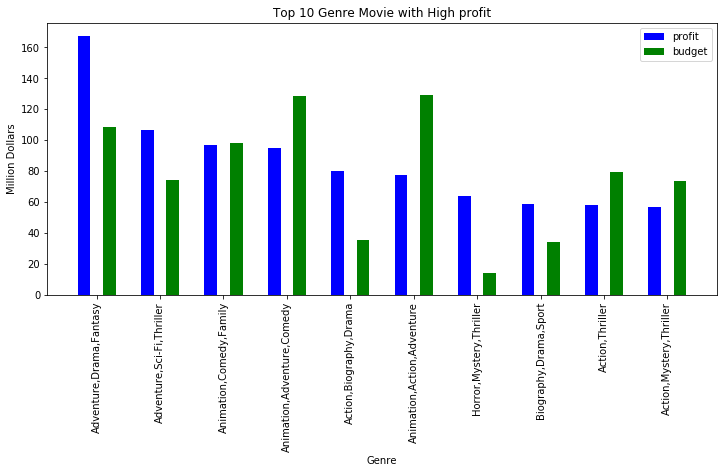
\includegraphics[scale=0.7]{bab4/top10highprofit_multibarchart}   
	\caption{10 kombinasi genre dengan perbandingan budget dan revenue tertinggi (profit) }
	\label{fig:top10highprofit_multibarchart} 
\end{figure} 

Gambar \ref{fig:top10highprofit_multibarchart} adalah visualisasi 10 kombinasi \textit{genre} terbaik dengan \textit{profit} tertinggi menggunakan \textit{barchart}. Visualisasi ini dapat memberikan \textit{feedback} kepada pembuat film kombinasi \textit{genre} mana saja yang menghasilkan \textit{profit}. Film \textit{Mystery, Horror} dan \textit{Thriller} adalah kombinasi \textit{genre} yang \textit{budget} yang dikeluarkan tidak terlalu tinggi tetapi masih menghasilkan keuntungan. Film yang mengandung \textit{genre animation} membutuhkan \textit{budget} yang besar tetapi masih menghasilkan keuntungan yang besar juga. Kombinasi \textit{genre} terbaik adalah \textit{"Adventure,Drama,Fantasy"}.

\subsection{Data Selection} 
\label{chap:hasiltambahandataselection}
Pada subbab ini dilakukan analisis korelasi terhadap kolom tambahan yaitu \textit{budget}, \textit{profit} dan \textit{roi} dengan fitur prediktor yang ada pada \textit{dataset}. Analisis dilakukan dengan 2 cara yaitu visualisasi korelasi dengan \textit{scatter plot} dan pengujian nilai \textit{pearson}. Fitur prediktor yang memiliki korelasi positif yang tinggi akan dipilih untuk menjadi prediktor untuk prediksi \textit{revenue},\textit{profit} dan \textit{roi}. 

Ingin dianalisis apakah \textit{budget} dan \textit{revenue} / pendapatan kotor memiliki korelasi positif satu sama lain. Berikut adalah visualisasi korelasi \textit{revenue} dan \textit{budget} dengan \textit{scatter plot}. 


\begin{figure}[H]
	\centering  
	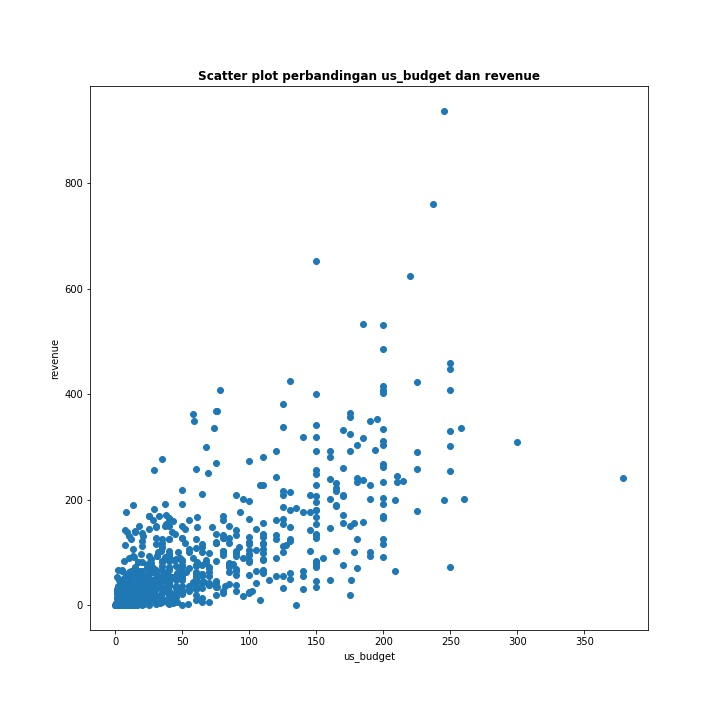
\includegraphics[scale=0.6]{bab4/budget_revenue_scatterplot}   
	\caption{Analisis korelasi kolom Budget dan Revenue}
	\label{fig:budget_revenue_scatterplot} 
\end{figure} 

Gambar \ref{fig:budget_revenue_scatterplot} menunjukkan bahwa \textit{budget} dan \textit{revenue} memiliki korelasi positif yang tinggi. Dapat dilihat semakin besar \textit{budget} yang dikeluarkan, maka semakin tinggi \textit{revenue} yang diperoleh. \textit{Budget} bisa menjadi salah satu fitur yang dapat dipilih untuk memprediksi \textit{revenue}. Berikut adalah pengujian korelasi tiap fitur prediktor dengan \textit{revenue} menggunakan \textit{pearson correlation} untuk memilih fitur prediksi terbaik. 


\begin{figure}[H]
	\centering  
	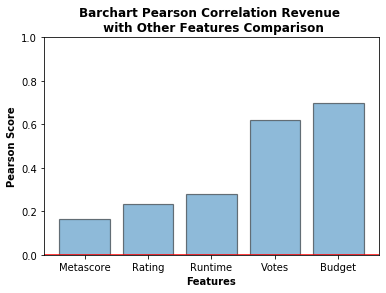
\includegraphics[scale=0.7]{bab4/pearson_iterasi2_revenue_barchart}   
	\caption{Pengujian perbandingan korelasi tiap fitur dengan revenue menggunakan pearson correlation ke-2}
	\label{fig:pearson_iterasi2_revenue_barchart} 
\end{figure} 

Gambar \ref{fig:pearson_iterasi2_revenue_barchart} adalah pengujian nilai \textit{pearson} tiap fitur prediktor dan target yaitu \textit{revenue} menggunakan \textit{barchart}. Berdasarkan pengujian sebelumnya pada subbab \ref{chap:hasilanalisisdatautama}, \textit{votes} merupakan fitur dengan nilai \textit{pearson}. Tetapi, fitur \textit{budget} ternyata lebih tinggi korelasinya dengan \textit{votes}. Berdasarkan penjelasan \textit{pearson} pada subbab \ref{chap:teori_pearsoncorrelation}, nilai \textit{pearson} terbaik adalah $1.0$. \textit{Budget} memiliki nilai korelasi yaitu $0.7$ sehingga memmiliki korelasi yang tinggi. Selain \textit{revenue},  dilakukan analisis korelasi fitur terhadap \textit{profit}. 
Berikut adalah visualisasi korelasi \textit{profit} dan fitur prediktor lain dengan \textit{scatter plot}. 


\begin{figure}[H]
    \centering
    \subfloat[Korelasi Rating dan Profit]{{\includegraphics[width=7cm]{bab4/rating_profit_scatterplot} }}%
    \qquad
    \subfloat[Korelasi Metascore dan Profit]{{\includegraphics[width=7cm]{bab4/metascore_profit_scatterplot} }}%
    \caption{Analisis korelasi situs review dan profit}%
    \label{fig:rating_metascore_profit_scatterplot}%
\end{figure}



\begin{figure}[H]
    \centering
    \subfloat[Korelasi Runtime dan Profit]{{\includegraphics[width=7cm]{bab4/runtime_profit_scatterplot} }}%
    \qquad
    \subfloat[Korelasi Votes dan Profit]{{\includegraphics[width=7cm]{bab4/votes_profit_scatterplot} }}%
    \caption{Analisis korelasi runtime votes dan profit}%
    \label{fig:runtime_votes_profit_scatterplot}%
\end{figure}

\begin{figure}[H]
	\centering  
	\includegraphics[scale=0.5]{bab4/budget_profit_scatterplot}   
	\caption{Analisis korelasi budget dan profit }
	\label{fig:budget_profit_scatterplot} 
\end{figure} 



Gambar \ref{fig:rating_boxplot}, \ref{fig:runtime_votes_profit_scatterplot} dan \ref{fig:budget_profit_scatterplot} adalah visualisasi korelasi tiap fitur dengan \textit{profit} menngunakan \textit{scatterplot}. Dibanding dengan korelasi \textit{revenue}, korelasi \textit{profit} dengan tiap fitur lebih tidak menunjukkan korelasi yang positif. Hal ini disebabkan karena setelah perhitungan \textit{profit} dengan selisih \textit{budget} dan \textit{revenue} banyak film yang menghasilkan kerugian sehingga korelasi positif berkurang. Berikut adalah pengujian korelasi \textit{profit} dengan fitur prediktor lain berdsarkan \textit{pearson correlation} menggunakan \textit{barchart}. 


\begin{figure}[H]
	\centering  
	\includegraphics[scale=0.7]{bab4/pearson_iterasi2_profit_barchart}   
	\caption{Pengujian perbandingan korelasi tiap fitur dengan profit menggunakan pearson correlation ke-2}
	\label{fig:pearson_iterasi2_profit_barchart} 
\end{figure} 

Berdasarkan Gambar \ref{fig:pearson_iterasi2_profit_barchart}, fitur yang memiliki korelasi positif tertinggi adalah \textit{votes}. Semakin banyak \textit{votes} sebuah film, maka semakin banyak \textit{profit} yang dapat diperoleh. Pengaruh dukungan penonton dapat mempengaruhi peningkatan \textit{profit}. Selain \textit{profit}, dilakukan analisis korelasi \textit{ROI} terhadap fitur prediktor lain menggunakan \textit{scatter plot}. 


\begin{figure}[H]
    \centering
    \subfloat[Korelasi Rating dan ROI]{{\includegraphics[width=7cm]{bab4/rating_roi_scatterplot} }}%
    \qquad
    \subfloat[Korelasi Metascore dan ROI]{{\includegraphics[width=7cm]{bab4/metascore_roi_scatterplot} }}%
    \caption{Analisis korelasi situs review dan ROI}%
    \label{fig:rating_metascore_roi_scatterplot}%
\end{figure}



\begin{figure}[H]
    \centering
    \subfloat[Korelasi Runtime dan ROI]{{\includegraphics[width=7cm]{bab4/runtime_roi_scatterplot} }}%
    \qquad
    \subfloat[Korelasi Votes dan ROI]{{\includegraphics[width=7cm]{bab4/votes_roi_scatterplot} }}%
    \caption{Analisis korelasi runtime votes dan roi}%
    \label{fig:runtime_votes_roi_scatterplot}%
\end{figure}



\begin{figure}[H]
	\centering  
	\includegraphics[scale=0.5]{bab4/budget_roi_scatterplot}   
	\caption{Analisis korelasi budget dan profit }
	\label{fig:budget_profit_scatterplot} 
\end{figure} 


Berdasarkan Gambar \ref{fig:rating_metascore_roi_scatterplot}, \ref{fig:runtime_votes_roi_scatterplot} dan \ref{fig:budget_profit_scatterplot}, banyak fitur prediktor yang tidak menunjukkan korelasi positif yang kuat dengan ROI. Berikut adalah pengujian korelasi \textit{ROI} dengan fitur prediktor berdasarkan \textit{pearson correlation} menggunakan \textit{barchart}. 


\begin{figure}[H]
	\centering  
	\includegraphics[scale=0.7]{bab4/pearson_iterasi2_roi_barchart}   
	\caption{Pengujian perbandingan korelasi tiap fitur dengan ROI menggunakan pearson correlation ke-2}
	\label{fig:pearson_iterasi2_roi_barchart} 
\end{figure} 


Berdasarkan Gambar \ref{fig:pearson_iterasi2_roi_barchart}, tidak ada fitur yang menunjukkan korelasi yang positif dengan \textit{ROI} karena nilai yang dihasilkan sangat kecil. Nilai korelasi yang kecil dan negatif pada beberapa fitur menyebabkan percobaan prediksi \textit{ROI} tidak dapat dilakukan.



\subsection{Percobaan Prediksi Fitur Data Tambahan}
Pada subbab ini dilakukan percobaan membuat model yang dapat memprediksi keuntungan film yaitu \textit{revenue} dan \textit{profit} menggunakan regresi. Percobaan prediksi regresi menggunakan \textit{Linear Regression} dan \textit{Polynomial Regression}. Berdasarkan hasil pengujian \textit{pearson} sebelumnya fitur yang paling berpengaruh adalah \textit{votes} dan \textit{budget} sehingga prediksi memanfaatkan 2 fitur sekaligus untuk membuat model prediksi.

\subsubsection{Percobaan Prediksi Revenue}
Berdasarkan \textit{training model} yang sudah dibuat. Berikut adalah perbandingan nilai R2 prediksi \textit{revenue} menggunakan \textit{votes} dan \textit{budget}. 

\begin{table}[H]
\caption{Tabel Skor R2 Revenue}
\centering
\begin{tabular}{|c|c|}
\hline 
\multicolumn{2}{|c|}{Fitur Prediktor : votes dan budget} \\ 
\hline 
Skor R2 Linear  & Skor R2 Polynom \\ 
\hline 
0.56 & 0.60 \\ 
\hline 
\end{tabular} 
\label{tab:tabelr2revenue_iterasi2}
\end{table}

Berdasarkan Tabel \ref{tab:tabelr2revenue_iterasi2}, skor evaluasi R2 pada iterasi ke-2 meningkat dibanding dengan skor R2  iterasi ke-1 pada Tabel \ref{tab:tabelr2_iterasi1}. Pada percobaan kali ini algoritma \textit{Polynomilal Regression} memiliki nilai R2 yang lebih tinggi dari \textit{Linear Regression}. Berikut adalah tabel percobaan prediksi \textit{revenue} pada model \textit{votes} dan \textit{budget}.

\begin{table}[H]
\caption{Tabel sampel percobaan prediksi Revenue menggunakan regresi fitur votes dan budget}
\centering
\begin{tabular}{|c|c|c|c|c|c|}
\hline 
Title & Votes & Budget & Revenue Asli & Revenue Linear & Revenue Polynomial \\ 
\hline 
Final Destination 5 & 88000 & 40 & 42.80 & 46.45 & 48.61 \\ 
\hline 
Twilight & 361449 & 37 & 191.45 & 99.61 & 94.15 \\ 
\hline 
Warm Bodies & 153579 & 33 & 66.36 & 53.73 & 58.105 \\ 
\hline 
17 Again & 152808 & 20 & 64.15 & 41.88 & 47.00 \\ 
\hline 
Spider-Man 3 & 406219 & 258 & 336.53 & 304 & 312 \\ 
\hline 
... & ... & ... & ... & ... & ... \\ 
\hline 
\end{tabular} 
\label{tab:5sampelprediksi_revenueiterasi2}
\end{table}

\subsubsection{Percobaan Prediksi Profit}
Berdasarkan \textit{training model} yang sudah dibuat. Berikut adalah perbandingan nilai R2 prediksi \textit{profit} menggunakan \textit{votes} dan \textit{budget}. 


\begin{table}[H]
\caption{Tabel skor R2 prediksi profit}
\centering
\begin{tabular}{|c|c|}
\hline 
\multicolumn{2}{|c|}{Fitur Prediktor : votes dan Budget} \\ 
\hline 
Skor R2 Linear & Skor R2 Polynomial \\ 
\hline 
0.20 & 0.29 \\ 
\hline 
\end{tabular} 

\label{tab:tabelr2_profit}
\end{table}

Berdasarkan hasil Tabel \ref{tab:tabelr2_profit}, nilai evaluasi R2 untuk memprediksi \textit{profit} memiliki nilai yang kecil sehingga tidak dapat digunakan untuk prediksi Berikut adalah perbandingan sampel percobaan prediksi \textit{profit} dengan \textit{profit} asli. 

\begin{table}[H]
\caption{Tabel sampel percobaan prediksi profit menggunakan budget dan votes dan perbandingannya dengan profit asli}
\centering
\begin{tabular}{|c|c|c|c|c|c|}
\hline 
Title & Votes & Budget & Profit Asli & Profit Linear  & Profit Polynomial \\ 
\hline 
Trolls & 38552 & 125 & 28.98 & -13.51 & -59.03 \\ 
\hline 
Diary of the Wimpy Kid & 34184 & 15 & 49 & -0.9 & 6.62 \\ 
\hline 
Goosebumps & 57602 & 67 & 13.02 & -2.9 & -12.29 \\ 
\hline 
Finding Dory & 157026 & 200 & 286.29 & -2.0 & -57.303 \\ 
\hline 
Piranha 3D & 75262 & 24 & 1 & 5.59 & 11.27 \\ 
\hline 
... & ... & ... & ... & ... & ... \\ 
\hline 
\end{tabular} 
\label{tab:5sampelprediksi_profititerasi2}
\end{table}

Berdasarkan Tabel \ref{tab:5sampelprediksi_profititerasi2}, Hasil prediksi yang dihasilkan untuk memprediksi \textit{profit} sangat buruk. Sehingga model yang dibuat dengan fitur yang terbaik tidak dapat digunakan untuk memprediksi \textit{profit}. 

\section{Proses Analisis Data Sosial Media} 
Berdasarkan informasi yang didapatkan pada Subbab \ref{chap:hasilanalisisdatatambahan}, fitur yang memiliki korelasi yang paling tinggi adalah \textit{votes} dan \textit{budget}. \textit{Votes} adalah jumlah pengguna situs IMDB yang suka / mendukung sebuah \textit{film} tetapi \textit{votes} hanya mencakup pendukung film yang tergabung dalam situs IMDB. Banyak penikmat film yang menyukai film tetapi tidak berkontribusi untuk menilai sebuah film pada situs IMDB. Akan dilakukan pengujian analisis kesuksesan film berdasarkan data sosial media.

Tahap-tahap yang dilakukan selama proses analisis data media sosial adalah : 

\begin{itemize}
\item Melakukan pengumpulan data media sosial \textit{Youtube} dan \textit{Instagram}

\item Melakukan \textit{data integration} untuk menggabungkan data media sosial dengan \textit{dataset}

\item Melakukan analisis data media sosial dengan menggunakan visualisasi 

\item Melakukan \textit{data selection} untuk memilih fitur terbaik prediksi \textit{revenue} dan \textit{profit} 

\item Melakukan prediksi \textit{revenue} dan \textit{profit} menggunakan fitur media sosial 
\end{itemize} 



Penjelasan secara lebih detail proses analisis data media sosial dijelaskan pada subbab berikutnya. Berdasarkan hasil analisis data media sosial yang dilakukan, informasi yang didapat adalah. 

\begin{itemize}
\item Pengumpulan data menggunakan API \textit{youtube}  sangat lambat karena ada batas kuota tiap harinya 
\item Pengumpulan data \textit{youtube} dan \textit{instagram} dapat menggunakan \textit{Octoparse} dan memanfaatkan \textit{url} dinamis dari halaman yang ingin dikumpulkan

\item Berdasarkan analisis \textit{dataset},Fitur \textit{view count} (\textit{Youtube}) lebih berpengaruh daripada dibanding \textit{hashtag (Instagram)}

\item Ada kecenderungan semakin banyak jumlah penonton \textit{trailer film} di \textit{youtube} (viewCount), maka semakin meningkat kemungkinan \textit{revenue} dan \textit{profit} yang dapat diperoleh. \textit{Trailer} sebuah film yang menarik dapat membuat penonton tertarik untuk menonton di bioskop


\item Ada kecenderungan popularitas aktor dalam media sosial khususnya \textit{instagram} memiliki pengaruh terhadap peningkatan \textit{revenue} sebuah film


\item \textit{Genre} film yang paling menguntungkan berdasarkan jumlah penonton \textit{trailer} di \textit{youtube} adalah \textit{Action,Adventure}.

\item Nilai evaluasi R2 prediksi \textit{revenue} meningkat dari 0.60 menjadi 0.65 setelah menambah data Youtube sebagai prediktor sehingga model prediksi sudah mendekati 0.70 yaitu minimum sebuah model yang dapat digunakan untuk model prediksi 

\item Nilai evaluasi R2 prediksi \textit{profit} meningkat dari 0.30 menjadi 0.38 setelah menambah fitur Youtube sebagai prediktor

\end{itemize}




\subsection{Data Collection}
\textit{Youtube} adalah \textit{platform} berbagi video secara gratis. Setiap pengguna dapat mengunggah video dan mendapatkan jumlah \textit{view} dan \textit{like} yang banyak.  \textit{Youtube} dapat menghitung jumlah \textit{view} yang ditonton oleh \textit{user.} Semakin banyak \textit{view} yang diperoleh maka semakin video itu akan direkomendasikan kepada \textit{user} lain.

Sebuah film membutuhkan media untuk mempromosikan film yang dibuat kepada penonton.  Biasanya pihak produksi \textit{film} akan menciptakan \textit{trailer} untuk mempromosikan film yang dibuat. \textit{Trailer} adalah cuplikan video tentang promosi film yang dilakukan sebelum film rilis ke bioskop. Pembuat film menciptakan akun \textit{youtube} dan mengunggah \textit{trailer} yang dibuat ke situs \textit{youtube}. Pada proses ini akan diuji apakah jumlah penonton \textit{trailer} film di \textit{youtube} dapat mempengaruhi kesuksesan film.

Selain \textit{youtube}, terdapat situs media sosial lain yang digunakan pembuat film untuk mempromosikan film. \textit{Instagram} adalah sebuah aplikasi berbagi foto dan video untuk para pengguna sosial media. \textit{Instagram} memiliki fitur berupa setiap \textit{user} dapat mengikuti \textit{user} lain (\textit{follow}). Semakin banyak \textit{follower} yang dimiliki, maka akan semakin terkenal sebuah akun. Selain fitur \textit{follow}, \textit{instagram} memiliki fitur \textit{hashtag}. \textit{Hashtag} (\#) adalah tagar yang dapat ditambahkan pada sebuah foto yang diunggah sehingga \textit{user} yang tidak saling \textit{follow} tetap dapat berbagi konten. 

Biasanya \textit{hashtag} digunakan untuk memberikan makna tema sebuah foto. Pembuat film akan memanfaatkan \textit{instagram} untuk mempromosikan film dengan mengunggah foto poster film dan video \textit{trailer} singkat. Pada proses ini diuji juga apakah sosial media \textit{instagram} memiliki pengaruh pada tingkat kesuksesan film. 


\subsubsection{Data Collection pada Youtube}
\textit{Google} menyediakan sebuah media bagi para \textit{developer} untuk mengambil data secara  \textit{open source}. \textit{Youtube} sebagai bagian dari \textit{google} menyediakan API yang dapat dimanfaatkan untuk mengambil data \textit{youtube} bernama \textit{YoutubeAPIV3}. Cara mendapatkan data adalah dengan melakukan \textit{request} pada \textit{uniform resource locator} (\textit{url}) yang disediakan \textit{youtube}. Contoh \textit{url} yang dapat diakses untuk melakukan pencarian data video adalah. 


\begin{displaymath}
https://www.googleapis.com/youtube/v3/search?part=snippet\& q=<query>\& key=<apikey>
\end{displaymath}

\textit{url} adalah \textit{request} yang dapat dilakukan untuk melakukan pencarian data. Teks "<query>" dan "<apikey>" dapat diubah secara dinamis. \textit{query} adalah kata kunci pencarian video dan \textit{apikey} adalah sebuah \textit{identifier} / penanda \textit{user} mana yang melakukan \textit{request} data. \textit{Apikey} dapat diperoleh dari registrasi \textit{API} dengan menggunakan akun \textit{gmail}. Hasil dari pencarian ini adalah sebuah teks \textit{json}.



\begin{figure}[H]
	\centering  
	\includegraphics[scale=0.7]{bab4/json_searchyoutubeexample}   
	\caption{Contoh JSON hasil request search youtube menggunakan API }
	\label{fig:json_searchyoutubeexample} 
\end{figure} 


Id video dari hasil pencarian pada dapat digunakan untuk memanggil \textit{request statistic}. \textit{Request statistic} adalah \textit{request} data video yang berhubungan dengan status video. \textit{Statistics} adalah data yang berhubungan dengan \textit{view}, jumlah \textit{likes} dan \textit{dislikes} sebuah video. \textit{Url} yang dapat diakses untuk mengambil datanya adalah. 



\begin{displaymath}
https://www.googleapis.com/youtube/v3/videos?part=statistics\& id= <video\textunderscore id>\& key=<apikey>
\end{displaymath}

\textit{Url} diatas dapat melakukan untuk mengambil data statistik sebuah video dari \textit{youtube}. \textit{Request} ini menerima parameter berupa \textit{video\textunderscore id} dan \textit{apikey}. \textit{Video id} adalah \textit{identifier} dari sebuah video. \textit{Video id}  yang sebelumnya diperoleh dari \textit{request} pencarian video dapat dimanfaatkan. Berdasarkan \textit{video id} yang sudah diperoleh untuk mengambil data \textit{"The dark knight trailer"} pada Gambar \ref{fig:json_searchyoutubeexample}, berikut adalah hasil pencarian data statistik. 

\begin{figure}[H]
	\centering  
	\includegraphics[scale=0.8]{bab4/json_getstatisticyoutubeexample}   
	\caption{Contoh JSON hasil request seach youtube menggunakan API }
	\label{fig:json_getstatisticyoutubeexample} 
\end{figure} 

Gambar \ref{fig:json_getstatisticyoutubeexample} adalah contoh hasil data statistik yang diperoleh dari pencarian "The dark knight trailer".  Berdasarkan penjelasan API untuk pencarian data \textit{youtube}, pengumpulan data \textit{view youtube} dari setiap \textit{trailer film} pada \textit{dataset}. 


\begin{figure}[H]
	\centering  
	\includegraphics[scale=0.8]{bab4/json_youtubequotaexceeded}   
	\caption{Contoh JSON Error Youtube Quota Exceeded }
	\label{fig:json_youtubequotaexceeded} 
\end{figure} 

Pada pencarian jumlah \textit{view trailer} pada \textit{dataset} ke-90, \textit{json} yang dikembalikan adalah \textit{json} pada Gambar \ref{fig:json_youtubequotaexceeded}. Hasil \textit{request} tersebut menjelaskan bahwa ternyata terdapat batas dalam melakukan \textit{request} tiap harinya. Maka, pencarian data sosial media menggunakan API tidak dapat dilakukan karena membutuhkan waktu untuk menunggu kuota dapat terisi kembali tiap harinya. Akan dilakukan \textit{scraping} menggunakan \textit{Octoparse} sebagai solusi lain. 

Untuk mengakses situs \textit{youtube} menggunakan \textit{browser}, \textit{user} memerlukan untuk memasukkan \textit{url} alamat situs \textit{youtube}. Contoh \textit{url} untuk melakukan pencarian pada film adalah. 


\begin{displaymath}
https://www.youtube.com/results?search_query=<kueri pencarian>
\end{displaymath} 

\textit{Url} diatas dapat dimanfaatkan untuk melakukan pencarian video \textit{youtube}. Bagian "<kueri pencarian>" adalah sebuah teks dinamis yang dapat diganti dengan \textit{query} pencarian dari video yang dibutuhkan. Dengan memanfaatkan \textit{url} ini, sehingga \textit{scraping} jumlah \textit{view trailer} video pada \textit{dataset} dapat dilakukan dengan \textit{Octoparse}. 

\begin{figure}[H]
	\centering  
	\includegraphics[scale=0.5]{bab4/youtubeview_scrap_octoparse}   
	\caption{Tampilan octoparse untuk scraping youtube view }
	\label{fig:youtubeview_scrap_octoparse} 
\end{figure} 

Gambar \ref{fig:youtubeview_scrap_octoparse} adalah tampilan saat \textit{Octoparse} memilih elemen dalam mengambil data. Dengan menggunakan cara ini, akan dilakukan pencarian semua data jumlah \textit{trailer film} pada \textit{dataset} menggunakan \textit{Octoparse}. Berikut adalah 10 sampel \textit{url} yang di\textit{generate} dari \textit{dataset}. 

\begin{table}[H]
\caption{10 sampel url yang digenerate}
\centering
\begin{tabular}{|c|}
 \hline 
\textbf{ Url Dataset yang diakses untuk scrapping} \\ 
 \hline 
 www.youtube.com/results?search\textunderscore query=Prometheus trailer  \\ 
 \hline 
 www.youtube.com/results?search\textunderscore query=Split trailer  \\ 
 \hline 
 www.youtube.com/results?search\textunderscore query=Sing trailer  \\ 
 \hline 
 www.youtube.com/results?search\textunderscore query=Suicide Squad trailer  \\ 
 \hline 
 www.youtube.com/results?search\textunderscore query=The Great Wall trailer  \\ 
 \hline 
 www.youtube.com/results?search\textunderscore query=La La Land trailer  \\ 
 \hline 
 www.youtube.com/results?search\textunderscore query=The Lost City of Z trailer  \\ 
 \hline 
 www.youtube.com/results?search\textunderscore query=Fantastic Beasts and Where to Find Them trailer  \\ 
 \hline 
 www.youtube.com/results?search\textunderscore query=Hidden Figures trailer  \\ 
 \hline 
 www.youtube.com/results?search\textunderscore query=Rogue One trailer  \\ 
 \hline 
 \end{tabular} 

\label{tab:10sampelurl_youtubetrailer}
\end{table} 

Tabel \ref{tab:10sampelurl_youtubetrailer} adalah beberapa dari semua \textit{url} yang akan diakses menggunakan \textit{octoparse}. \textit{Octoparse} mengakses semua \textit{url dataset} untuk mengambil data jumlah \textit{view} dari \textit{trailer} film. Dengan memanfaatkan \textit{octoparse} dan semua \textit{url} yang di\textit{generate}, berikut adalah contoh 10 sampel hasil pencarian jumlah \textit{view trailer}. 


\begin{table}[H]
\centering
\caption{10 sampel hasil \textit{scrapping} \textit{youtube view} menggunakan \textit{octoparse}} 
\begin{tabular}{|l|c|}
\hline 
\textbf{Youtube title} &\textbf{ Views} \\ 
\hline 
Prometheus - Official Full Trailer - In Theaters 6/8/12
 & 10M views
 \\ 
\hline 
Split Official Trailer 1 (2017) - M. Night Shyamalan Movie
 & 27M views
 \\ 
\hline 
Sing TRAILER 1 (2016) - Scarlett Johansson, Matthew McConaughey 
 & 9.1M views
 \\ 
\hline 
Suicide Squad - Official Trailer 1 [HD]
 & 90M views
 \\ 
\hline 
The Great Wall - Official Trailer 2 - In Theaters This February
 & 10M views
 \\ 
\hline 
La La Land (2016 Movie) Official Trailer – 'Dreamers'
 & 37M views
 \\ 
\hline 
The Lost City of Z International Trailer 1 (2017)  Movieclips Trailers
 & 6.3M views
 \\ 
\hline 
PASSENGERS - Official Trailer (HD) & 30M views
 \\ 
\hline 
Fantastic Beasts and Where to Find Them - Teaser Trailer [HD]
 & 16M views
 \\ 
\hline 
Hidden Figures  Official Trailer [HD]  20th Century FOX
 & 7.5M views
 \\ 
\hline 
\end{tabular} 

\label{tab:10sampelhasil_scrapyoutubeview}
\end{table}

Tabel \ref{tab:10sampelhasil_scrapyoutubeview} adalah beberapa contoh hasil \textit{scraping} untuk mengambil data \textit{youtube view}. Terdapat komponen lain dalam video \textit{youtube} seperti jumlah \textit{likes} dan \textit{dislikes} tetapi tidak semua video mau untuk ditampilkan jumlah \textit{like} sehingga analisis hanya menggunakan jumlah \textit{view}.

\subsubsection{Data Collection Instagram}
Fitur \textit{hashtag} \textit{Instagram} memungkinkan pengguna yang tidak berhubungan dapat membagikan foto dan video dengan tema yang sama. Tren suatu \textit{keyword hashtag} dapat mempengaruhi popularitas sesuatu hal. Contohnya adalah sebagai berikut.



\begin{figure}[H]
	\centering  
	\includegraphics[scale=0.6]{bab4/contohhashtag_instagram}   
	\caption{Contoh fitur Hashtag Instagram }
	\label{fig:contohhashtag_instagram} 
\end{figure} 

Gambar \ref{fig:contohhashtag_instagram} adalah contoh sebuah tren \textit{hashtag} dengan \textit{keyword} sebuah film yaitu \textit{"Guardians of the Galaxy"}. Semua unggahan foto dengan \textit{hashtag} "Guardians of the galaxy" adalah semua hal yang berhubungan dengan film tersebut seperti aktor, poster dan video unggahan. Pada tahap ini dilakukan pengumpulan data menggunakan \textit{Octoparse}. \textit{Url instagram} yang diakses dengan \textit{url} tertentu 


\begin{displaymath}
https://www.instagram.com/explore/tags/<namahashtag>/
\end{displaymath} 

\textit{url} \textit{hashtag instagram} dapat dimanfaatkan untuk mengakses sebuah halaman dengan \textit{hashtag} tertentu. Bagian "<namahashtag>" dapat diganti sesuai \textit{hashtag} yang ingin diakses. Dengan menggunakan \textit{url} yang disediakan \textit{instagram}, akan dibuat seluruh \textit{url hashtag} berdasarkan nama film pada \textit{dataset}. Berikut adalah sampel 10 \textit{url instagram hashtag} berdasarkan film \textit{dataset}.

\begin{table}[H]
\caption{10 Sampel URL Instagram Hashtag dengan Menggunakan Judul Film}
\centering
 \begin{tabular}{|c|}
 \hline 
 url Hashtag Instagram \\ 
 \hline 
  https://www.instagram.com/explore/tags/TheComedian/  \\ 
 \hline 
  https://www.instagram.com/explore/tags/SpringBreakers/  \\ 
 \hline 
  https://www.instagram.com/explore/tags/Hairspray/  \\ 
 \hline 
  https://www.instagram.com/explore/tags/TheHappening/  \\ 
 \hline 
 https://www.instagram.com/explore/tags/TheAssassinationofJesseJamesbytheCowardRobertFord/  \\ 
 \hline 
 https://www.instagram.com/explore/tags/Fridaythe13th/  \\ 
 \hline 
 https://www.instagram.com/explore/tags/KickAss/  \\ 
 \hline 
 https://www.instagram.com/explore/tags/SuckerPunch/  \\ 
 \hline 
 https://www.instagram.com/explore/tags/RocknRolla/  \\ 
 \hline 
 https://www.instagram.com/explore/tags/BlueValentine/  \\ 
 \hline 
 \end{tabular} 

\label{tab:10sampel_urljudulhashtaginstagram}
\end{table}

Tabel \ref{tab:10sampel_urljudulhashtaginstagram} adalah beberapa \textit{url} yang diakses untuk mengambil jumlah \textit{hashtag} dari \textit{keyword} judul film dari \textit{dataset}. Semua \textit{url} yang berjumlah 838 \textit{url hashtag} film akan diakses oleh \textit{Octoparse}. Berikut adalah sampel 10 hasil \textit{scraping} yang peroleh \textit{Octoparse}. 

\begin{table}[H]
\centering
\caption{10 Sampel hasil \textit{scraping } data hashtag instagram  menggunakan \textit{octoparse}}
\begin{tabular}{|c|c|}
  \hline 
  Hashtag Judul Film & Jumlah Post \\ 
  \hline 
  \# thecomedian & 27,932 \\ 
  \hline 
  \# springbreakers & 268,282 \\ 
  \hline 
  \# hairspray & 708,045 \\ 
  \hline 
  \# thehappening & 11,619 \\ 
  \hline 
  \# theassanisation & 1,940 \\ 
  \hline 
  \# fridaythe13th & 2,497,489 \\ 
  \hline 
  \# kickass & 1,228,185 \\ 
  \hline 
  \# suckerpunch & 109,806 \\ 
  \hline 
  \# rocknrolla & 137,870 \\ 
  \hline 
  \# bluevalentine & 47,173 \\ 
  \hline 
  \end{tabular}   

\label{tab:10sampel_hasilscrapjudulinstagram}
\end{table}

Tabel \ref{tab:10sampel_hasilscrapjudulinstagram} adalah beberapa contoh hasil \textit{scraping} untuk mengambil jumlah \textit{hashtag} dari setiap judul film pada \textit{dataset}. Selain pengumpulan jumlah data \textit{hashtag} judul film, akan dilakukan pengumpulan data \textit{hashtag}  dengan \textit{keyword} nama aktor/aktris utama pada sebuah film. Aktor/ aktris umumnya sudah memiliki situs sosial media resmi untuk berhubungan dengan penggemarnya. Biasanya aktor akan bekerja sama dengan pembuat film untuk mempromosikan filmnya melalui sosial media. Dengan cara yang sama seperti melakukan \textit{scraping} \textit{hashtag} judul film, akan dilakukan pengumpulan data \textit{hashtag} nama aktor. Berikut adalah 10 sampel film beserta \textit{hashtag} aktor yang diakses. 

\begin{table}[H]
\caption{10 Sampel hasil pengumpulan data \textit{hashtag} aktor utama setiap film pada dataset}
\centering
\begin{tabular}{|c|}
\hline 
url hashtag aktor utama  \\ 
\hline 
 https://www.instagram.com/explore/tags/robertdeniro/  \\ 
\hline 
 https://www.instagram.com/explore/tags/vanessahudgens/  \\ 
\hline 
 https://www.instagram.com/explore/tags/johntravolta/  \\ 
\hline 
 https://www.instagram.com/explore/tags/markwahlberg/  \\ 
\hline 
https://www.instagram.com/explore/tags/bradpitt/  \\ 
\hline 
https://www.instagram.com/explore/tags/jaredpadalecki/  \\ 
\hline 
https://www.instagram.com/explore/tags/aarontaylorjohnson/  \\ 
\hline 
https://www.instagram.com/explore/tags/emilybrowning/  \\ 
\hline 
https://www.instagram.com/explore/tags/gerardbutler/  \\ 
\hline 
https://www.instagram.com/explore/tags/ryangosling/  \\ 
\hline 
\end{tabular} 

\label{tab:10sampel_urlscrapaktorhashtag}
\end{table}

Tabel \ref{tab:10sampel_urlscrapaktorhashtag} adalah beberapa contoh dari semua \textit{url} yang di\textit{generate} untuk mengakses semua \textit{hashtag} aktor utama film pada \textit{dataset}. Setelah melakukan \textit{scraping} dengan \textit{Octoparse}, berikut adalah 10 sampel jumlah \textit{hashtag actor}.

\begin{table}[H]
\centering
\caption{10 Sampel hasil \textit{scraping} data \textit{hashtag} aktor dengan \textit{Octoparse} }
\begin{tabular}{|c|c|}
\hline 
Hashtag Actor & Jumlah Post \\ 
\hline 
\# robertdeniro & 424,802 \\ 
\hline 
\# vanessahudgens & 478,292 \\ 
\hline 
\# johntravolta & 241,526 \\ 
\hline 
\# markwahlberg & 197,163 \\ 
\hline 
\# bradpitt & 1,055,192 \\ 
\hline 
\# jaredpadalecki & 4,068,673 \\ 
\hline 
\# aarontaylorjohnson & 93,604 \\ 
\hline 
\# emilybrowning & 22,936 \\ 
\hline 
\# gerardbutler & 143,321 \\ 
\hline 
\# ryangosling & 774,215 \\ 
\hline 
\end{tabular} 

\label{tab:10sampel_hasilscrapactorhashtag}
\end{table}
 
Tabel \ref{tab:10sampel_hasilscrapactorhashtag} adalah beberapa sampel hasil \textit{scraping} data \textit{hashtag} aktor yang diperoleh. Data yang diperoleh merupakan jumlah unggahan foto dari semua \textit{user} yang menggunakan \textit{hashtag} tersebut. 

\subsection{Data Integration}
Terdapat 3 fitur sosial media yang sudah diperoleh selama tahap \textit{data collection} yaitu : 

\begin{itemize}
\item Jumlah \textit{view count trailer (Youtube)}
\item Jumlah \textit{hashtag count title (Instagram)}  
\item Jumlah \textit{hashtag count actor name (Instagram)}
\end{itemize}

Data sosial media yang sudah diperoleh sebelumnya digunakan untuk digabungkan dengan \textit{dataset}. Cara penggabungan adalah dengan memanfaatkan judul film pada \textit{dataset} dan nama aktor utama. Berikut adalah contoh beberapa \textit{dataset} yang telah tergabung dengan data sosial media. 

\begin{table}[H]
\caption{Sampel data integrasi antara \textit{dataset} dengan data sosial media}
\centering
\begin{tabular}{|c|c|c|c|c|}
\hline 
Title & ... & Youtube Trailer View & Hashtag title & Hashtag Actor \\ 
\hline 
Kickboxer: Vengeance & ... & 4.5M Views & 3,122 & 65,443 \\ 
\hline 
Spider-Man 3 & ... & 4.5M Views & 138,212 & 205,845 \\ 
\hline 
Hercules & ... & 1.9M Views & 1,0737,96 & 645,185 \\ 
\hline 
The Amazing Spider-Man & ... & 14M Views & 414,847 & 389,582 \\ 
\hline 
In the Heart of the Sea & ... & 12M Views & 137,475 & 1,457,829 \\ 
\hline 
The Lost City of Z & ... & 6.3M Views & 94,449 & 355,403 \\ 
\hline 
Turbo Kid & ... & 668K Views & 17,222 & 20,625 \\ 
\hline 
Fool's Gold & ... & 21M Views & 150,990 & 172,612 \\ 
\hline 
Monster Trucks & ... & 4.4M Views & 370,426 & 23,660 \\ 
\hline 
Men in Black 3 & ... & 17M Views & 9,118 & 1,391,216 \\ 
\hline 
\end{tabular} 
\label{tab:10sampel_dataintegrasiiterasi3}
\end{table}

Tabel \ref{tab:10sampel_dataintegrasiiterasi3} menunjukkan bahwa \textit{dataset} sudah digabungkan dengan data sosial media.

\subsection{Data Transformation} 
Data sosial media yang sudah digabung dengan \textit{dataset} akan dianalisis menggunakan visualisasi, tetapi terdapat beberapa masalah yaitu  :

\begin{itemize}
\item Data \textit{youtube view} masih berbentuk \textit{String} (contoh: "1.2 M Views")
\item Data \textit{youtube view} masih memiliki variasi data yang berbeda (Contoh : "1.2M" untuk satuan jutaan dan "333K" untuk satuan ribuan)
\item Data \textit{Instagram Hashtag} masih berbentuk \textit{String} ("120,000") 
\end{itemize}

Berdasarkan permasalahan data sosial media yang dijelaskan sebelumnya, maka dilakukan \textit{data transformation} untuk mengubah data media sosial menjadi bentuk yang lebih sesuai. Berikut adalah tabel konversi 3 kolom sosial media pada \textit{dataset}. 

\begin{table}[H]
\caption{Operasi dan contoh data \textit{transformation} pada data media sosial}
\centering
\begin{tabular}{|c|c|c|c|}
\hline 
Nama Kolom & Operasi & Sebelum Konversi &  Sesudah Konversi \\ 
\hline 
Youtube View & Menghilangkan keyword "M,K" & 1.4M Views & 1.4 \\ 

 & Mengubah dalam bentuk satuan jutaan & 300K Views & 0.3 \\ 
\hline 
Hashtag Title  & Mengubah tipe data menjadi numerik & "120,000" & 120000 \\ 
\hline 
Hashtag Actor & Mengubah tipe data menjadi numerik & "10,000" & 10000 \\ 
\hline 
\end{tabular} 
\label{tab:operasi_datatransformation_iterasi3}
\end{table}




Tabel \ref{tab:operasi_datatransformation_iterasi3} adalah detail operasi yang dilakukan untuk mengonversi data sosial media menjadi bentuk yang lebih tepat agar dapat dianalisis secara deskriptif. Perubahan fitur media sosial menjadi numerik agar fitur media sosial dapat dianalisis secara visualisasi. Kolom \textit{youtube view} dibuat menjadi satuan jutaan. Kolom \textit{hashtag Instagram} dirubah dari \textit{String} menjadi numerik. Berikut adalah contoh 5 sampel pada \textit{dataset}.

\begin{table}[H]
\caption{5 Sampel \textit{dataset} setelah konversi \textit{data transformation} }
\centering
\begin{tabular}{|c|c|c|c|}
\hline 
Title & Youtube\textunderscore view (jutaan) & Hashtag Title & Hashtag Actor \\ 
\hline 
Deadpool & 19 & 5622065 & 585034 \\ 
\hline 
Ant-Man & 25 & 1534586 & 276859 \\ 
\hline 
Sherlock Holmes & 2 & 1948636 & 2469813 \\ 
\hline 
Hands of Stone & 0.297 & 27155 & 393655 \\ 
\hline 
RED & 0.962 & 115604667 & 280856 \\ 
\hline 
\end{tabular} 
\label{tab:5sampel_hasildatatransformation_iterasi3}
\end{table}

Tabel \ref{tab:5sampel_hasildatatransformation_iterasi3} adalah contoh beberapa hasil \textit{dataset} yang sudah di\textit{transform} menjadi bentuk yang lebih sesuai. 


\subsection{Analisis Data Media Sosial Menggunakan Visualisasi}
Berdasarkan data sosial media yang sudah diperoleh pada subbab sebelumnya, akan dilakukan analisis data menggunakan visualisasi. Berikut adalah visualisasi distribusi fitur media sosial menggunakan \textit{boxplot}. 

\subsubsection{Analisis Visualisasi Youtube View Count}
\begin{figure}[H]
	\centering  
	\includegraphics[scale=0.6]{bab4/viewCount_boxplot}   
	\caption{Boxplot view count}
	\label{fig:viewCount_boxplot} 
\end{figure} 

Gambar \ref{fig:viewCount_boxplot} adalah visualisasi distribusi menggunakan \textit{boxplot}. Tiap film memiliki jumlah banyak pengguna yang menonton \textit{trailer} film tersebut di situs \textit{youtube}. Berdasarkan visualisasi terdapat film-film divisualisasikan sebagai \textit{outlier} karena terlalu jauh dari nilai Q2. Berikut adalah 5 film \textit{outlier}\textit{view count} tertinggi. 

\begin{table}[H]
\caption{5 Film \textit{outlier} dengan \textit{View Count} Terbanyak}
\centering
\begin{tabular}{|c|c|c|c|c|}
\hline 
Title & Genre & Revenue (Million) & ROI (\%) & View\\ 
\hline 
Star Wars : The Force Awakens  & Action,Adventure,Fantasy & 936.63 & 282.298 & 105 \\ 
\hline 
Fifty Shades of Grey & Drama,Romance & 166.15 & 315.375 & 	95 \\ 
\hline 
Suicide Squad & Action, Adventure,Fantasy & 325.02 & 85.72 &90 \\ 
\hline 
Jurrasic World & Action,Adventure,Sci-fi & 652.18 & 334.7867 &89 \\ 
\hline 
Avengers: Age of Ultron & Action,Adventure,Sci-Fi & 408.08 & 83.596 &88\\ 
\hline 
\end{tabular} 
\label{tab:5film_viewcountterbaik}
\end{table}
%
Tabel \ref{tab:5film_viewcountterbaik} adalah 5 film \textit{outlier} dengan jumlah \textit{view} \textit{trailer youtube} yang tertinggi. 5 film terbaik berdasarkan \textit{view count} cenderung merupakan film \textit{genre} \textit{Action} dan \textit{Adventure}. Film terbaik berdasarkan \textit{view} juga meraih \textit{revenue} dan \textit{ROI} yang menguntungkan.

\subsubsection{Analisis Visualisasi Instagram Hashtag Title}

\begin{figure}[H]
	\centering  
	\includegraphics[scale=0.7]{bab4/instagram_hashtagtitle_boxplot}   
	\caption{Hashtag Instagram title boxplot }
	\label{fig:instagram_hashtagtitle_boxplot} 
\end{figure} 

Gambar \ref{fig:instagram_hashtagtitle_boxplot} adalah \textit{boxplot} dari \textit{hashtag title} \textit{Instagram}. Berdasarkan \textit{boxplot} yang diberikan, terdapat film yang memiliki \textit{hashtag} yang jumlahnya sangat tinggi. Berikut adalah 5 film \textit{outlier} dengan \textit{hashtag title} terbanyak.

\begin{table}[H]
\caption{5 Film \textit{outlier} berdasarkan Hashtag judul terbanyak}
\centering
\begin{tabular}{|c|c|c|c|}
\hline 
Title & Hashtag Title Instagram & Revenue & ROI \\ 
\hline 
Vacation & 116,583,160 & 58.88 & 282.533 \\ 
\hline 
RED & 115,604,667 & 90.36 & 55.79 \\ 
\hline 
Sunshine & 67,897,892 & 3.68 & -29.86 \\ 
\hline 
Australia & 61,052,897 & 49.55 & -80.45 \\ 
\hline 
Gold & 55,697,911 & 7.22 & -12.78 \\ 
\hline 
\end{tabular} 
\label{tab:5film_hashtagtitleterbanyak}
\end{table}

Tabel \ref{tab:5film_hashtagtitleterbanyak} adalah 5 fim dengan \textit{hashtag} terbanyak berdasarkan judul. Film yang memiliki \textit{hashtag} judul banyak cenderung tidak menunjukkan pola yang menarik. Hal ini disebabkan karena judul film merupakan \textit{term} / kata yang sering muncul dan bukan judul film khusus.

\subsubsection{Analisis Visualisasi Hashtag Actor Instagram}

\begin{figure}[H]
	\centering  
	\includegraphics[scale=0.7]{bab4/instagram_hashtagactor_boxplot}   
	\caption{Hashtag Instagram actor boxplot }	\label{fig:instagram_hashtagactor_boxplot} 
\end{figure} 

Gambar \ref{fig:instagram_hashtagactor_boxplot} adalah \textit{boxplot} untuk distribusi \textit{hashtag actor} utama dalam setiap film pada \textit{dataset}. \textit{Hashtag actor} menunjukkan popularitas seorang aktor. Berikut adalah 5 film yang aktor utama memiliki \textit{hashtag} terbanyak.


\begin{table}[H]
\caption{5 Film \textit{outlier} berdasarkan \textit{Actor Hashtag} terbanyak}
\centering
\begin{tabular}{|c|c|c|c|c|}
\hline 
Title & Aktor & Jumlah Hashtag & Revenue & ROI \\ 
\hline 
Friday the 13th & Jared Padalecki & 4.068.673 & 65 & 242,10 \\ 
\hline 
The Maze Runner & Dylan O Brien & 3.271.395 & 102,41 & 201,20 \\ 
\hline 
Fifty Shades of Grey & Dakota Johnson & 3.235.549 & 166,15 & 315,38 \\ 
\hline 
Iron Man & Robert Downey  & 2,469813 & 318,3 & 127,36 \\ 
\hline 
Captain America : Civil War & Chris Evans & 2.444.525 & 408,08 & 63.232 \\ 
\hline 
\end{tabular} 
\label{fig:5terbaik_actorhashtaginstagram}
\end{table}

Tabel \ref{fig:5terbaik_actorhashtaginstagram} adalah 5 film \textit{outlier} berdasarkan popularitas aktor di \textit{Instagram} berdasarkan \textit{jumlah hashtag}. Aktor yang populer di\textit{instagram} cenderung film yang dimainkan menghasilkan keuntungan.

\subsubsection{Tren Youtube View Trailer Dari Tahun Ke Tahun}

\begin{figure}[H]
	\centering  
	\includegraphics[scale=0.7]{bab4/youtubeview_yearbyyear_lineplot}   
	\caption{Analisis tren\textit{ youtube view} \textit{trailer}}
	\label{fig:youtubeview_yearbyyear_lineplot} 
\end{figure} 

Gambar \ref{fig:youtubeview_yearbyyear_lineplot} adalah visualisasi tren jumlah \textit{view trailer youtube} setiap film pada \textit{dataset} dari tahun ke tahun. Berdasarkan visualisasi, akumulasi \textit{view} dari tahun ke tahun meningkat. Peminat situs \textit{youtube} untuk menonton \textit{trailer} film yang mereka tunggu-tunggu semakin meningkat. Pihak pembuat film dapat memanfaatkan media sosial untuk dapat mempromosikan film.

\subsubsection{Tren Instagram Hashtag Dari Tahun Ke Tahun}
\begin{figure}[H]
	\centering  
	\includegraphics[scale=0.7]{bab4/instagramhashtag_yearbyyear_lineplot}   
	\caption{Analisis tren\textit{ Instagram Hashtag }}	\label{fig:instagramhashtag_yearbyyear_lineplot} 
\end{figure} 

Gambar \ref{fig:instagramhashtag_yearbyyear_lineplot} adalah visualisasi tren \textit{instagram hashtag} dari tahun ke tahun. Jumlah akumulasi unggahan foto/video tiap tahunnya meningkat. Meningkatnnya tiap tahun dapat dimanfaatkan pihak pembuat film untuk fokus  mempromosikan filmnya di  \textit{instagram}.

\subsection{Data Selection} 
Visualisasi korelasi semua fitur satu sama lain. Visualisasi ditampilkan menggunakan \textit{heatmap}.

 
\begin{figure}[H]
	\centering  
	\includegraphics[scale=0.7]{bab4/heatmap_all_feature}   
	\caption{Pearson correlation fitur prediktor terhadap \textit{revenue}}	\label{fig:heatmap_all_feature} 
\end{figure}

Gambar \ref{fig:heatmap_all_feature} adalah visualisasi korelasi tiap fitur. Warna biru menandakan korelasi positif dan merah menandakan korelasi negatif. Semakin gelap warnanya menandakan korelasi semaki kuat. Berdasarkan hasil visualisasi \textit{heatmap}, informasi yang didapatkan adalah : 

\begin{itemize}
\item Ada kecenderungan jika nilai \textit{metascore} yang diperoleh sebuah film tinggi, maka semakin tinggi \textit{rating} yang diperoleh 

\item Jumlah \textit{post} pada \textit{hashtag instagram} yang menggunakan judul film (\textit{hashtagcount} tidak memiliki pengaruh terhadap fitur lain 


\item Semakin banyak \textit{budget} yang dikeluarkan, maka ada kemungkinan sebuah film dapat dibuat dengan durasi lebih lama. Hal ini disebabkan oleh proses penyuntingan film yang lebih lama dan membutuhkan biaya lebih

\item Semakin banyak \textit{budget} yang dikeluarkan, maka akan kemungkinan \textit{votes} sebuah film meningkat
 
\item Ada kecenderungan semakin banyak \textit{budget} yang dikeluarkan, maka semakin meningkat jumlah penonton \textit{trailer film} di \textit{youtube}. Pembuatan \textit{trailer} yang menarik dapat meningkatkan minat penonton

\item Semakin banyak jumlah penonton \textit{trailer film} di \textit{youtube} (viewCount), maka semakin meningkat \textit{revenue} dan \textit{profit} yang dapat diperoleh. \textit{Trailer} sebuah film yang menarik dapat membuat penonton tertarik untuk menonton di bioskop

\item Semakin banyak \textit{votes} yang diperoleh, maka semakin banyak \textit{revenue} dan \textit{profit} yang diperoleh 

\item Tidak terdapat fitur yang memiliki  korelasi yang kuat terhadap \textit{ROI}  

\item Ada kecenderungan semakin banyak jumlah \textit{post} dengan menggunakan \textit{hashtag} nama aktor utama film, maka semakin meningkat keuntungan sebuah film. Pembuat film dapat bekerjasama menggunakan akun resmi sosial media para aktor untuk membantu mempromosikan film
\end{itemize}

Pada tahap ini dilakukan pengujian korelasi semua fitur prediktor media sosial dengan target kesuksesan yaitu \textit{revenue,profit} dan \textit{ROI} menggunakan \textit{pearson correlation}. Berikut adalah pengujian \textit{pearson} fitur prediktor terhadap \textit{revenue} menggunakan visualisasi. 

\subsubsection{Pearson Correlation Revenue Dengan Fitur Lain}

\begin{figure}[H]
	\centering  
	\includegraphics[scale=0.7]{bab4/pearson_iterasi3_revenue_barchart}   
	\caption{Pearson correlation fitur prediktor terhadap \textit{revenue}}	\label{fig:pearson_iterasi3_revenue_barchart} 
\end{figure}


Gambar \ref{fig:pearson_iterasi3_revenue_barchart} adalah hasil visualisasi perbandingan perhitungan nilai korelasi \textit{pearson correlation} tiap fitur terhadap \textit{revenue} menggunakan \textit{barchart}. Berdasarkan visualisasi yang ditunjukkan, \textit{budget} / pengeluaran memiliki nilai korelasi yang paling tinggi. Data media sosial seperti \textit{view trailer youtube} juga menjadi salah satu fitur yang mempengaruhi kenaikan \textit{revenue} dibanding fitur lain. \textit{Hashtag} judul film pada \textit{Instagram} dinilai tidak memiliki korelasi dengan \textit{revenue} 

\subsubsection{Pearson Correlation Profit Dengan Fitur Lain}

\begin{figure}[H]
	\centering  
	\includegraphics[scale=0.7]{bab4/pearson_iterasi3_profit_barchart}   
	\caption{Pearson correlation fitur prediktor terhadap \textit{profit}}	\label{fig:pearson_iterasi3_profit_barchart} 
\end{figure}


Gambar \ref{fig:pearson_iterasi3_profit_barchart} adalah hasil visualisasi perbandingan nilai korelasi \textit{pearson correlation} tiap fitur dan \textit{profit} menggunakan \textit{barchart}. Nilai korelasi yang paling tinggi adalah \textit{votes} dan \textit{view count}. Data media sosial yaitu \textit{trailer youtube (viewCount)} menjadi salah satu prediktor yang memiliki korelasi yang kuat dengan \textit{profit}. Data media sosial ternyata dapat dipertimbangkan menjadi fitur yang berpengaruh terhadap \textit{revenue} dan \textit{profit}


\subsubsection{Pearson Correlation ROI Dengan Fitur Lain}
\begin{figure}[H]
	\centering  
	\includegraphics[scale=0.7]{bab4/pearson_iterasi3_roi_barchart}   
	\caption{Pearson correlation fitur prediktor terhadap \textit{profit}}	\label{fig:pearson_iterasi3_roi_barchart} 
\end{figure}

Gambar \ref{fig:pearson_iterasi3_roi_barchart} adalah hasil visualisasi perbandingan nilai korelasi tiap fitur dan \textit{ROI}. Berdasarkan hasil visualisasi, tidak terdapat fitur yang memiliki korelasi yang kuat dengan \textit{ROI}. Nilai tertinggi hanya \textit{metascore} dengan nilai \textit{pearson} yaitu $0.10$. Nilai \textit{pearson} \textit{metascore} dan \textit{ROI} tidak dapat diklasifikasikan sebagai korelasi yang kuat. Terdapat beberapa fitur yang memiliki nilai korelasi negatif dengan \textit{ROI}. Data media sosial tidak memiliki pengaruh terhadap \textit{ROI}. 


\subsection{Percobaan Prediksi Fitur Data Sosial Media}
Pada subbab ini dilakukan percobaan membuat model regresi dengan memanfaatkan fitur media sosial \textit{viewCount}. Model regresi dibuat agar dapat memprediksi keuntungan film yaitu \textit{revenue} dan \textit{profit}. 

\subsubsection{Prediksi Revenue Menggunakan Linear Regression Dengan Data Media Sosial} 
\textit{Dataset} dibagi menjadi 2 bagian \textit{training} dan \textit{test}. \textit{Dataset} dibagi menjadi 80 persen dan 20 persen \textit{test}. Data \textit{training} digunakan untuk menghasilkan fungsi regresi dari prediksi. Dengan menambah \textit{viewCount} sebagai fitur tambahan, fungsi regresi berdasarkan data \textit{training} yang dihasilkan \textit{linear regression} untuk memprediksi \textit{revenue} adalah 

\begin{equation}
revenueLinearRegression = -11.67 + 0.00019 (votes) + 0.82 * (budget) + 1.19 (viewCount)
\label{eqref:fungsilinear_revenue_iterasi3}
\end{equation}

Persamaan \ref{eqref:fungsilinear_revenue_iterasi3} adalah fungsi yang dihasilkan untuk melakukan percobaan prdiksi pendapatan kotor / \textit{revenue}. Fungsi ini memanfaatkan 3 fitur yaitu \textit{votes}, \textit{budget} dan \textit{viewCount}. Berikut adalah 5 data film yang diambil dari data \textit{test} dan hasil prediksinya menggunakan fungsi \textit{Linear Regression}. 

\begin{table}[H]
\caption{Tabel percobaan \textit{Linear Regression} untuk prediksi \textit{revenue} menggunakan fitur \textit{votes,budget} dan \textit{viewCount} }
\centering
\begin{tabular}{|c|c|c|c|c|c|}
\hline 
Title & Votes & Budget & ViewCount & Revenue Asli & Revenue Prediksi \\ 
\hline 
Sherlock Holmes &357436 & 123 & 1.4 & 186.83 & 162.234 \\ 
\hline 
Victor Frankenstein & 37975 & 65 & 9.8 & 5.77 & 60.89 \\ 
\hline 
Pirates of the Caribbean &498821 & 300 & 1.8 & 309.4 & 334.156 \\ 
\hline 
Final Destination 5 & 88000 & 40 & 0.07 & 42.58 & 38.40 \\ 
\hline 
Grown Ups 2 & 114482 & 80 & 3.8 & 133.67 & 80.91 \\ 
\hline 
\end{tabular} 
\label{tab:5sampel_prediksirevenue_linear_iterasi3}
\end{table}

Tabel \ref{tab:5sampel_prediksirevenue_linear_iterasi3} dapat digunakan untuk melihat perbandingan \textit{revenue} asli dan hasil prediksi yang diihasilkan oleh \textit{Linear regression} menggunakan fitur \textit{votes,budget} dan \textit{viewCount}. Berikut adalah distribusi nilai \textit{squared error} dari percobaan semua prediksi data \textit{test}.

\begin{figure}[H]
	\centering  
	\includegraphics[scale=0.7]{bab4/squarederror_linear_revenue_iterasi3_boxplot}   
	\caption{Distribusi nilai \textit{squared errors} ($(ypred-ytest)^2$) \textit{Linear regression} pada prediksi \textit{revenue} menggunakan fitur \textit{votes,budget} dan \textit{viewCount}}	\label{fig:squarederror_linear_revenue_iterasi3_boxplot} 
\end{figure}

Gambar \ref{fig:squarederror_linear_revenue_iterasi3_boxplot}
menunjukkan persebaran nilai \textit{squared error} memiliki nilai yang tidak terlalu besar. Nilai Skor akurasi R2 yang diperoleh adalah.

\begin{table}[H]
\centering
\caption{Hasil nilai R2 \textit{linear regression} pada prediksi revenue menggunakan data sosial media }
\begin{tabular}{|c|}
 \hline 
 R2 prediksi Revenue Linear Regression data sosial media\\ 
 \hline 
 0.63 \\ 
 \hline 
 \end{tabular}  
 \label{tab:r2_linear_revenue_iterasi3}
\end{table}

Tabel \ref{tab:r2_linear_revenue_iterasi3} adalah hasil skor akurasi prediksi \textit{revenue} menggunakan algoritma \textit{linear regression}. Terdapat peningkatan skor R2 setelah menambah fitur media sosial yaitu \textit{viewCount}. 

\subsubsection{Prediksi Revenue Menggunakan Polynomial Regression Dengan Data Media Sosial}
Percobaan prediksi \textit{revenue} menggunakan fitur sosial media juga diuji dengan \textit{polynomial regression}. Fungsi prediksi yang dihasilkan adalah. 

\begin{equation}
\begin{split}
revenuePolynomialRegression = 2.88 + 0.00015 * (votes)  + 0.58 * (budget) + 0.81 * (viewCount) + \\ 0.00000000002 * (votes)^2 +  0.0000023 (votes) (budget) +  0.0000012 (votes)(viewCount) + \\  0.0023 (budget)^2 + 0.0021 (budget)(viewCount) + 0.0037 (viewCount)^2 
\end{split}
\label{eqref:fungsipolinom_revenue_iterasi3}
\end{equation}


Persamaan \ref{eqref:fungsipolinom_revenue_iterasi3} adalah fungsi yang dihasilkan untuk melakukan percobaan prediksi pendapatan kotor / \textit{revenue} menggunakan \textit{polynomial regression}. Berikut adalah 5 data film yang diambil dari data \textit{test} dan hasil prediksinya menggunakan fungsi \textit{polynomial regression}


\begin{table}[H]
\caption{Tabel percobaan \textit{Polynomial Regression} untuk prediksi \textit{revenue} menggunakan fitur \textit{votes,budget} dan \textit{viewCount}} 
\centering
\begin{tabular}{|c|c|c|c|c|c|}
\hline 
Title & Votes & Budget & ViewCount & Revenue Asli & Revenue Prediksi \\ 
\hline 
Sherlock Holmes & 357436 & 123 & 1.4 & 186.83 & 176.784 \\ 
\hline 
Victor Frankenstein & 37975 & 65 & 9.8 & 5.77 & 52.077 \\ 
\hline 
Pirates of the Caribbean & 498821 & 300 & 1.8 & 309.4 & 356.95 \\ 
\hline 
Final Destination & 88000 & 40 & 0.07 & 42.58 & 42.84 \\ 
\hline 
Grown Ups 2 & 11482 & 80 & 3.8 & 133.67 & 75.87 \\ 
\hline 
\end{tabular} 
\label{tab:5sampel_prediksirevenue_polinom_iterasi3}
\end{table}

Tabel \ref{tab:5sampel_prediksirevenue_polinom_iterasi3} menampilkan percobaan prediksi pada 5 data \textit{test}. Terdapat prediksi yang sangat akurat dan ada yang perbandingan \textit{revenue} asli dan prediksi yang memiliki selisih yang jauh. Berikut adalah distribusi nilai \textit{squared error} dari percobaan semua prediksi data \textit{test}. 



\begin{figure}[H]
	\centering  
	\includegraphics[scale=0.7]{bab4/squarederror_polinom_revenue_iterasi3_boxplot}   
	\caption{Distribusi nilai \textit{squared errors} ($(ypred-ytest)^2$) \textit{Polynomial regression} pada prediksi \textit{revenue} menggunakan fitur \textit{votes,budget} dan \textit{viewCount}}	\label{fig:squarederror_polinom_revenue_iterasi3_boxplot} 
\end{figure}

Gambar \ref{fig:squarederror_polinom_revenue_iterasi3_boxplot}
adalah distribusi nilai \textit{squared error} yang diperoleh dari percobaan prediksi \textit{revenue} \textit{polynomial regression} menggunakan fitur data sosial media. Berdasarkan nilai Q2, percobaan pada \textit{linear regression} memiliki \textit{squared error } yang lebih kecil. Nilai akurasi R2 yang diperoleh adalah. 


\begin{table}[H]
\centering
\caption{Hasil nilai R2 \textit{polynomial regression} pada prediksi revenue menggunakan data sosial media }
\begin{tabular}{|c|}
\hline 
R2 prediksi Revenue Polynomial Regression data sosial media \\ 
\hline 
0.65 \\ 
\hline 
\end{tabular} 
\label{tab:r2_polinom_revenue_iterasi3}
\end{table}

Tabel \ref{tab:r2_polinom_revenue_iterasi3} adalah hasil skor akurasi prediksi \textit{revenue} menggunakan algoritma \textit{polynomial regression}. Hasil R2 yang diperoleh meningkat lebih tinggi dibanding \textit{linear regression} dan prediksi pada Data Utama pada iterasi sebelumnya. Data sosial media terbukti memiliki pengaruh dalam kesuksesan film 


\subsubsection{Prediksi Profit Menggunakan Linear Regression Dengan Data Media Sosial}
 
Selain \textit{revenue}, dilakukan pengujian prediksi \textit{profit} menggunakan \textit{linear regression} dan \textit{polynomial regression}. Fitur prediktor yang digunakan adalah 3 fitur terbaik yaitu \textit{votes,budget} dan \textit{viewCount}. Fungsi prediksi yang dihasilkan \textit{linear regression} untuk memprediksi \textit{profit} adalah. 


\begin{equation}
profitLinearRegression = -11.67 + 0.00019 (votes) + (-0.17)(budget) + 1.19 * (viewCount) 
\label{eqref:fungsilinear_profit_iterasi3}
\end{equation}

Persamaan \ref{eqref:fungsilinear_profit_iterasi3} adalah fungsi yang dihasilkan untuk menghitung prediksi \textit{profit}. Fitur yang digunakan adalah \textit{votes},\textit{budget} dan \textit{viewCount}. Berikut adalah 5 data film yang diambil dari data \textit{test} dan perbandingan prediksinya menggunakan \textit{Linear Regression}.

\begin{table}[H]
\caption{Tabel percobaan \textit{Linear Regression} untuk prediksi \textit{profit} menggunakan fitur \textit{votes,budget} dan \textit{viewCount}} 
\centering
\begin{tabular}{|c|c|c|c|c|c|}
\hline 
Title & Votes & Budget & viewCount & Profit Asli  & Profit Prediksi \\ 
\hline 
Sherlock Holmes & 357436 & 125 & 1.4 & 61.83 & 37.23 \\ 
\hline 
Victor Frankenstein & 37975 & 65 & 9.8 & -59.23 & -4.10 \\ 
\hline 
Pirates of the Caribbean & 498821 & 300 & 1.8 & 9.4 & 34.15 \\ 
\hline 
Final Destination & 88000 & 40 & 0.07 & 2.58 & -1.59 \\ 
\hline 
Grown Ups 2 & 114482 & 80 & 3.8 & 53.67 & 0.91 \\ 
\hline 
\end{tabular} 
\label{tab:5sampel_prediksiprofit_linear_iterasi3}
\end{table}

Tabel \ref{tab:5sampel_prediksiprofit_linear_iterasi3} merupakan data \textit{test} dan hasil perbandingan \textit{profit} asli dan prediksi menggunakan \textit{linear regression}. Hasil prediksi yang diperoleh masih kurang baik dibanding saat memprediksi \textit{revenue}. Berikut adalah distribusi \textit{squared error} yang diperoleh pada Gambar \ref{fig:squarederror_linear_profit_iterasi3_boxplot}.

 
\begin{figure}[H]
	\centering  
	\includegraphics[scale=0.7]{bab4/squarederror_linear_profit_iterasi3_boxplot}   
	\caption{Distribusi nilai \textit{squared errors} ($(ypred-ytest)^2$) \textit{Linear regression} pada prediksi \textit{profit} menggunakan fitur \textit{votes,budget} dan \textit{viewCount}}	\label{fig:squarederror_linear_profit_iterasi3_boxplot} 
\end{figure}

Berikut adalah nilai R2 dari prediksi \textit{profit} menggunakan \textit{Linear Regression}. 

\begin{table}[H]
\centering
\caption{Hasil nilai R2 \textit{linear regression} pada prediksi \textit{profit} menggunakan data sosial media }
\begin{tabular}{|c|}
\hline 
R2 prediksi Profit Linear Regression data sosial media \\ 
\hline 
0.34 \\ 
\hline 
\end{tabular} 
\label{tab:r2_linear_profit_iterasi3}
\end{table}

Nilai yang diperoleh \ref{tab:r2_linear_profit_iterasi3} masih cukup kecil untuk disebut sebagai prediksi yang akurat karena masih lebih kecil dari $0.7$. 


\subsubsection{Prediksi Profit Menggunakan Polynomial Regression Dengan Data Media Sosial}

Percobaan prediksi \textit{profit} juga diuji dengan \textit{polynomial regression}. Fungsi prediksi yang dihasilkan adalah. 

\begin{equation}
\begin{split}
profitPolynomialRegression = 2.88  + 0.00015 (votes) + \\ (-0.41) (budget) + 0.81 (viewCount) + (-0.00000000021) (votes)^2  +\\ 0.0000024 (votes)(budget) + 0.0000012 (votes)(viewCount) + (-0.0023) (budget) ^ 2 + \\ 0.0021 (budget)(viewCount) + (-0.0037) (viewCount) ^2
\end{split}
\label{eqref:fungsipolinom_profit_iterasi3}
\end{equation}

Persamaan \ref{eqref:fungsipolinom_profit_iterasi3} adalah fungsi yang dihasilkan untuk melakukan percobaan prediksi \textit{profit} menggunakan \textit{polynomial regression}. Berikut adalah percobaan 5 data \textit{test} menggunakan \textit{Polynomial Regression}

\begin{table}[H]
\caption{Tabel percobaan \textit{Polynomial Regression} untuk prediksi \textit{profit} menggunakan fitur \textit{votes,budget} dan \textit{viewCount}} 
\centering
\begin{tabular}{|c|c|c|c|c|c|}
\hline 
Title & Votes & Budget & View Count & Profit Asli & Profit Prediksi \\ 
\hline 
Sherlock Holmes & 357436 & 125 & 1.4 & 61.83 & 51.78 \\ 
\hline 
Victor Frankenstein & 37975 & 65 & 9,8 & -59.23 & -12.9225 \\ 
\hline 
Pirates of the Caribbean & 498821 & 300 & 1.8 & 9.4 & 56.95 \\ 
\hline 
Final Destination & 88000 & 40 & 0.07 & 2.58 & 2.94 \\ 
\hline 
Grown Ups 2 & 114482 & 80 & 3.8 & 54.67 & -4.12 \\ 
\hline 
\end{tabular} 
\label{tab:5sampel_prediksiprofit_polinom_iterasi3}
\end{table}

Tabel \ref{tab:5sampel_prediksiprofit_polinom_iterasi3} menunjukkan hasil percobaan prediksi \textit{profit} menggunakan fungsi prediksi yang dihasilkan. Hasil yang dimiliki polinom lebih baik dari linear. Berikut adalah nilai distribusi \textit{squared error} dari percobaan fungsi prediksi data \textit{test} pada 
Gambar \ref{fig:squarederror_polinom_profit_iterasi3_boxplot} menggunakan \textit{boxplot} .


\begin{figure}[H]
	\centering  
	\includegraphics[scale=0.7]{bab4/squarederror_polinom_profit_iterasi3_boxplot}   
	\caption{Distribusi nilai \textit{squared errors} ($(ypred-ytest)^2$) \textit{Polynomial regression} pada prediksi \textit{profit} menggunakan fitur \textit{votes,budget} dan \textit{viewCount}}	\label{fig:squarederror_polinom_profit_iterasi3_boxplot} 
\end{figure}

Selain distribusi nilai \textit{squared error}
, berikut adalah skor akurasi R2 dari \textit{polynomial regression} menggunakan data media sosial.

\begin{table}[H]
\centering
\begin{tabular}{|c|}
\hline 
R2 prediksi Profit Polynomial Regression data sosial media \\ 
\hline 
0.38 \\ 
\hline 
\end{tabular} 
\label{tab:tab:r2_linear_profit_iterasi3}
\end{table}

\pagebreak

\section{Analisis Clustering} 
Pada subbab ini dilakukan implementasi \textit{clustering} pada \textit{dataset}. Hasil \textit{cluster} dianalisis untuk mengambil informasi seperti sifat \textit{cluster} yang dihasilkan dan interpretasinya. \textit{Clustering} dilakukan berdasarkan 2 fitur yaitu \textit{genre} dan \textit{aktor}.

\subsection{Clustering Berdasarkan Aktor} 
\textit{Clustering} berdasarkan aktor dilakukan untuk mengetahui sebuah kelompok dengan pasangan aktor yang sering bermain bersama. Fitur aktor pada \textit{dataset} merupakan tipe data \textit{String} berisi nama aktor yang dipisah berdasarkan koma. 

\begin{table}[H]
\caption{Contoh Aktor pada \textit{Dataset}}
\centering
\begin{tabular}{|c|c|}
\hline 
Title & Aktor \\ 
\hline 
Guardians of The Galaxy & Chris Pratt,Vin Diesel, Bradley Cooper, Zoe Saldana \\ 
\hline 
Star Trek Beyond        & Chris Pine, Zachary Quinto, Karl Urban, Zoe Saldana \\
\hline

\end{tabular} 
\label{tab:cluster_predataaktor}
\end{table}

Berdasarkan Tabel \ref{tab:cluster_predataaktor}, data aktor masih dalam bentuk \textit{String} sehingga perlu untuk diubah dalam bentuk numerik agar \textit{clustering} dapat dilakukan. Berdasarkan Subbab \ref{chap:teori_onehotencoding}, \textit{one hot encoding} dapat digunakan untuk mengubah data kategori  menjadi numerik sehingga dapat menghitung kemunculan aktor pada suatu film. 


\begin{table}[H]
\centering
\caption{ Contoh Hasil One Hot Encoding Aktor}
\resizebox{\textwidth}{!}{%
\begin{tabular}{|c|c|c|c|c|c|c|c|}
\hline 
Title  & Chris Pratt & Vin Diesel & Bradley Cooper & Zoe Saldana & Chris Pine & Karl Urban & Zachary Quinto \\ 
\hline 
Guardians of The Galaxy & 1 & 1 & 1 & 1 & 0 & 0 & 0 \\ 
\hline 
Star Trek Beyond & 0 & 0 & 0 & 1 & 1 & 1 & 1 \\ 
\hline 
\end{tabular} }
\label{tab:cluster_hasilonehotencodingaktor}
\end{table}

Tabel \ref{tab:cluster_hasilonehotencodingaktor} adalah contoh hasil konversi fitur aktor menjadi numerik menggunakan \textit{one hot encoding}. \textit{One hot encoding} dilakukan untuk semua film pada \textit{dataset} sehingga semua aktor dapat dihitung kemunculannya masing-masing. Untuk tiap baris film, nilai 0 menandakan bahwa aktor tersebut tidak bermain pada film sedangkan 1 menandakan bahwa aktor tersebut bermain terlibat dalam film. \textit{Hasil} \textit{one hot encoding} aktor digunakan untuk melakukan \textit{clustering} menggunakan \textit{K-Means} dan \textit{Agglomerative}. 

Perhitungan jarak tiap data objek / data film akan menggunakan \textit{cosine distance}. \textit{Cosine} digunakan karena ingin memenuhi syarat jika 2 film terdapat aktor yang sama, maka nilai jarak akan meningkat / semakin mirip. 

Algoritma \textit{K-Means} dan \textit{Agglomeratives} menerima \textit{input} berupa K / jumlah kelompok yang ingin dibuat. Jumlah nilai K yang dipilih mempengaruhi hasil \textit{cluster} / seberapa baik kemiripan antar anggota pada \textit{cluster}. Pada tahap ini dilakukan pengujian untuk menentukan nilai K terbaik menggunakan \textit{Silhouette score}. 


\begin{figure}[H]
	\centering  
	\includegraphics[scale=0.5]{bab4/kmeans_silhouettefindk_actorcluster}   
	\caption{Kualitas Clustering Aktor berdasarkan jumlah menggunakan \textit{Silhouette Score} }	\label{fig:kmeans_silhouettefindk_actorcluster} 
\end{figure}

Pengujian menentukan nilai K berdasarkan \textit{Silhouette score} pada \textit{barchart} Gambar \ref{fig:kmeans_silhouettefindk_actorcluster} menunjukkan bahwa nilai kualitas \textit{cluster} sangat buruk. Tiap bar merepresentasikan percobaan nilai K dan hasil uji yang diperoleh. Hal yang menyebabkan buruknya hasil \textit{cluster} adalah \textit{silhouette score} merupakan rata-rata dan penggabungan dari kualitas inter dan intra pada semua \textit{cluster}.  Kualitas \textit{cluster} yang buruk disebabkan oleh sebuah film yang memiliki masing-masing 2-4 aktor dan jarang terjadi kemungkinan 2 film yang semua aktornya sama persis. Yang dibutuhkan pada saat ini adalah tiap \textit{cluster} setidaknya terdapat satu aktor yang sama / berpasangan sehingga dilakukan pengujian \textit{intracluster} . Berikut adalah distribusi nilai \textit{intracluster} pada setiap percobaan nilai K pada \textit{cluster} aktor.


\begin{figure}[H]
	\centering  
	\includegraphics[scale=0.7]{bab4/intracluster_findk_clusteractor}   
	\caption{Distribusi nilai \textit{intracluster} pada beberapa percobaan clustering actor }	\label{fig:intracluster_findk_clusteractor} 
\end{figure}


Berdasarkan \textit{boxplot} Gambar \ref{fig:intracluster_findk_clusteractor}, nilai K yang paling tepat untuk menghasilkan \textit{cluster} sesuai kebutuhan adalah K = 200. Distribusi pada K =300 dan K=400 tidak sesuai karena jika dilihat pada distribusinya 2 daerah yaitu yang nilai \textit{intraclusternya} sangat buruk ( \textit{intracluster} < 0.2) dan sisanya yang sangat bagus (  0.9 <= \textit{intracluster} <= 1). Sifat distribusi tersebut akan menghasilkan satu \textit{cluster} yang besar tetapi anggotanya tidak memiliki keunikan dan sisa \textit{cluster} lain yang anggotanya hanya 1. Jika memilih K = 200 akan memenuhi persyaratan dimana setidaknya salah satu aktor yang bermain 2 film akan tergabung dalam satu \textit{cluster}. Selain pemilihan jumlah K, berikut adalah perbandingan performa \textit{clustering K-Means} dan \textit{Agglomeratives}.



\begin{table}[H]
\centering
\caption{Perbandingan waktu \textit{clustering} menggunakan KMeans dan Agglomeratives}
\begin{tabular}{|c|c|}
\hline 
 Waktu KMeans & Waktu Agglomeratives \\ 
\hline 
752 detik & 9 detik \\ 
\hline 
\end{tabular} 
\label{tab:perbandinganwaktu_clustering}
\end{table}


Berdasarkan Tabel \ref{tab:perbandinganwaktu_clustering} , \textit{clustering} aktor dengan menggunakan \textit{Agglomerative} lebih cepat dari \textit{KMeans}. \textit{Agglomerative clustering} lebih cepat karena setiap iterasi penggabungan anggota mengurangi jumlah anggota yang harus digabungkan sedangkan \textit{K-Means} setiap iterasi tetap menghitung jarak tiap data dengan \textit{centroid} sesuai jumlah data. Hasil \textit{clustering} memberikan sebuah label pada tiap data film yang berupa numerik dari 0-199. Berikut adalah distribusi jumlah anggota tiap kelompok dari hasil \textit{clustering} aktor.


\begin{figure}[H]
	\centering  
	\includegraphics[scale=0.7]{bab4/distribusijumlahanggota_actorcluster_histogram}   
	\caption{Distribusi jumlah anggota tiap \textit{cluster} aktor}	\label{fig:membercountdistribution_agglo_clusteractor} 
\end{figure}

\textit{Barchart} Gambar \ref{fig:membercountdistribution_agglo_clusteractor} adalah distribusi jumlah anggota tiap \textit{cluster} aktor. Sumbu y adalah frekuensi / jumlah kelompok pada suatu batang dan sumbu x adalah kelas jumlah anggota. Terdapat banyak kelompok yang anggotanya masih sendiri disebabkan tidak ada pasangan aktor yang mirip.


\begin{table}[H]
\caption{Contoh Anggota \textit{Cluster} 13,28 dan 161 hasil \textit{cluster Actor}}
\resizebox{\textwidth}{!}{%
\begin{tabular}{|c|c|c|c|c|c|c|c|c|c|c|}
\hline 
\parbox{2cm}{intracluster} & \parbox{1cm}{label} & \parbox{2cm}{title}  & \parbox{3cm}{actors} & \parbox{1.5cm}{runtime} & \parbox{1cm}{votes} & \parbox{1cm}{rating} & \parbox{1.5cm}{metascore} & \parbox{1cm}{revenue} & \parbox{1cm}{profit} & \parbox{1.5cm}{genre} \\ 
\hline 
0.61 & 13 & \parbox{1.5cm}{Iron Man}& \parbox{3cm}{ Robert Downey Jr., Gwyneth Paltrow, Terrence Howard, Jeff Bridges
}& 126 & 737719 &7.9 & 79 & 318.8 & 178 & \parbox{1.5cm}{ Action, \\ Adventure, \\ Sci-Fi}
 \\ 
\hline 
0.61 & 13 & Iron Man 2 & \parbox{3cm}{Robert Downey Jr., Mickey Rourke, Gwyneth Paltrow,Don Cheadle}
 & 124 & 556666& 7 & 57 & 312.06 & 112.06 & \parbox{1.5cm}{Action, \\ Adventure, \\ Sci-fi}
 \\ 
\hline 
0.61 & 13 & \parbox{1.5cm}{Iron Man 3} & \parbox{3cm}{Robert Downey Jr., Guy Pearce, Gwyneth Paltrow,Don Cheadle}
 & 130 & 591023 & 7.2 & 62 & 408.99 & 208 & \parbox{1.5cm}{Action,\\ Adventure,\\Sci-fi}
 \\ 
\hline 
0.51 & 161 & \parbox{1.5cm}{ Hotel \\ Transylvania 2}
 & \parbox{3cm}{Adam Sandler, \\ Andy Samberg,\\  Selena Gomez, \\ Kevin James}
 & 89 & 69157 & 6.7 & 44 & 169 & 89 & \parbox{1.5cm}{ Animation, \\ Comedy, \\ Family}
 \\ 
\hline 
0.51 & 161 &  \parbox{1.5cm}{Just Go \\ with It}
 & \parbox{3cm}{Adam Sandler, \\ Jennifer Aniston,\\  Brooklyn Decker, \\Nicole Kidman}
 & 117 & 182069 & 6.4 & 33 & 103.33 & 23 & \parbox{1.5cm}{Comedy, \\ Romance}
 \\ 
\hline 
0.51 & 161 & \parbox{1,5cm}{ Grown \\ Ups 2}
 & \parbox{3cm}{ Adam Sandler, \\ Kevin James, \\  Chris Rock, \\ David Spade}
 & 101 & 114482 & 5.4 & 19 & 133 & 53 & Comedy
 \\ 
\hline 
0.79 &28& \parbox{1.5cm}{ Trolls}

 &\parbox{3cm}{ Anna Kendrick, Justin Timberlake,Zooey Deschanel, Christopher Mintz-Plasse
}
 & 92 & 38552 & 6.5& 56 & 153.69 & 28.69 & \parbox{1.5cm}{Animation,\\Adventure,\\Comedy
}
 \\ 
\hline 
0.79 & 28 & \parbox{1.5cm}{Gabor Csupo \\
 }
 & \parbox{3cm}{Josh Hutcherson, AnnaSophia Robb, Zooey Deschanel, Robert Patrick}
 & 96 & 117297
 & 7.2 & 74 & 82.23 & 65.23 & \parbox{1.5cm}{Adventure, \\ Drama, \\ Family}
 \\ 
\hline 

\end{tabular} }
\label{tab:contohclusteractor_3kelompok}
\end{table}


Tabel \ref{tab:contohclusteractor_3kelompok} adalah contoh 3 dari 200 kelompok  hasil \textit{cluster} berdasarkan aktor yaitu kelompok 13,161 dan 28. Masing-masing \textit{cluster} terbukti memiliki aktor dominan contohnya \textit{cluster} 13 memiliki aktor dominan yang sering muncul adalah Robert Downey Jr. , \textit{cluster} 161 adalah Adam Sandler dan \textit{cluster} 28 adalah Zooey Deschanel. Selain mengetahui aktor dominan untuk tiap \textit{cluster}, dapat diketahui juga \textit{genre} favorit dari tiap aktor seperti Robert Downey Jr. paling banyak bermain di\textit{genre} \textit{Action,Adventure} dan \textit{Sci-fi} . Adam Sandler paling sering bermain di\textit{genre} \textit{Comedy} dan Zooey Deschanel paling sering bermain \textit{genre} \textit{Adventure}. 


Hasil \textit{cluster} aktor perlu diinterpretasi untuk mengetahui makna dari tiap \textit{cluster}. Terdapat beberapa temuan interpretasi dari hasil analisis \textit{cluster} aktor.


\subsubsection{ Tiap Cluster Merepresentasikan 1 Aktor Representatif}
Pengujian pertama adalah memastikan jika 1 \textit{cluster} merepresentasikan 1 aktor dominan. Aktor dominan dihitung berdasarkan kontribusi jumlah film dimana suatu aktor tergabung dalam suatu \textit{cluster}. Contoh jika pada sebuah \textit{cluster} terdapat 4 film dan Aktor "A" terlibat dalam satu film, maka kontribusi jumlah "A" dalam \textit{cluster} tersebut adalah 25 persen.  

\begin{equation}
Kontribusi(actor,cluster) =  \frac{Jumlah film yang actor mainkan di cluster}{Jumlah semua film pada cluster} * 100
\label{eqref:rumuskontribusi_jumlahfilm_clusteraktor}
\end{equation}



Persamaan \ref{eqref:rumuskontribusi_jumlahfilm_clusteraktor} adalah cara menghitung kontribusi seorang aktor pada \textit{cluster} tersebut Batas yang ditentukan jika seorang aktor adalah  aktor dominan dalam sebuah \textit{cluster} jika kontribusinya lebih dari 50 persen. Akan dihitung perbandingan jumlah \textit{cluster} yang memenuhi syarat dan tidak, untuk menguji kebenaran temuan. 


\begin{figure}[H]
	\centering  
	\includegraphics[scale=0.6]{bab4/hypothesis1_actorcontributiontitle_clusteractor_piechart}   
	\caption{Pengujian sebuah cluster merepresentasikan satu aktor dominan}	\label{fig:hypothesis1_actorcontributiontitle_clusteractor_piechart} 
\end{figure}


Gambar \ref{fig:hypothesis1_actorcontributiontitle_clusteractor_piechart} adalah hasil  visualisasi pengujian tiap \textit{cluster} merepresentasikan aktor utama menggunakan \textit{piechart}. Dari 200 \textit{cluster} aktor, $99.5$ persen (199 \textit{cluster}) memiliki seorang aktor yang kontribusi jumlah filmnya lebih dari 50 persen. Dapat disimpulkan \textit{cluster} dapat digunakan untuk menemukan aktor dominan. Seorang aktor dominan lebih sering bermain film dibanding yang lain sehingga metode ini dapat digunakan untuk menemukan pasangan aktor dominan yang bagus. Ada kemungkinan berbeda pasangan main akan mempengaruhi kualitas dan pendapatan film. 



Visualisasi \textit{word cloud} dapat membantu menemukan aktor dominan pada sebuah \textit{cluster}. Semakin besar nama seorang aktor maka artinya aktor tersebut adalah aktor utama dari \textit{cluster}. 

 

\begin{figure}[H]
	\centering  
	\includegraphics[scale=0.6]{bab4/wordcloud-actorlabel-13.0}   
	\caption{Wordcloud distribusi aktor cluster 13 }
	\label{fig:wordcloud-actorlabel-13.0} 
\end{figure} 



\begin{figure}[H]
	\centering  
	\includegraphics[scale=0.6]{bab4/wordcloud-actorlabel-28.0}   
	\caption{Wordcloud distribusi aktor cluster 28 }
	\label{fig:wordcloud-actorlabel-28.0} 
\end{figure} 



\begin{figure}[H]
	\centering  
	\includegraphics[scale=0.6]{bab4/wordcloud-actorlabel-161.0}   
	\caption{Wordcloud distribusi aktor cluster 161 }
	\label{fig:wordcloud-actorlabel-161.0} 
\end{figure} 

\subsubsection{ Aktor Representatif Memiliki Genre Favorit}
Berdasarkan temuan sebelumnya, sebuah \textit{cluster} memiliki aktor representatif. Pada tahap ini  diuji apakah aktor dominan memiliki \textit{genre} favorit. \textit{Genre} favorit adalah jumlah kontribusi sebuah \textit{genre} pada suatu \textit{cluster} lebih dari 50 persen. Kontribusi dapat dihitung dengan rumus sebagai berikut. 

\begin{equation}
Kontribusi(G,cluster) = \frac{Jumlah Film yang terdapat genre G pada cluster}{jumlah semua film pada cluster} * 100
\label{eqref:rumuskontribusi_genre_clusteraktor}
\end{equation}

Persamaan \ref{eqref:rumuskontribusi_genre_clusteraktor} digunakan untuk menghitung kontribusi \textit{genre} pada sebuah film. Pada tahap ini dilakukan perhitungan kontribusi tiap \textit{genre} pada masing-masing \textit{cluster}. \textit{Genre} yang paling muncul dan kontribusi diatas 50 persen maka disebut sebagai \textit{genre} favorit dalam sebuah \textit{cluster}. Dengan mengkombinasikan aktor dominan dengan \textit{genre} yang memiliki kontribusi di atas 50 persen, maka sebuah aktor dominan memiliki \textit{genre} favorit. Pada tahap ini juga akan dihitung jumlah \textit{cluster} yang memenuhi syarat kontribusi \textit{genre} di atas 50 persen. Berikut adalah visualisasi distribusi kontribusi \textit{genre} favorit dari tiap \textit{cluster} untuk pengujian setiap aktor memiliki \textit{genre} favorit.


\begin{figure}[H]
	\centering  
	\includegraphics[scale=0.6]{bab4/hypothesis2_actorfavoritegenre_clusteractor}   
	\caption{Pengujian aktor dominan memiliki \textit{genre} favorit pada tiap \textit{cluster}}	
\label{fig:hypothesis2_actorfavoritegenre_clusteractor} 
\end{figure}

Berdasarkan \textit{piechart} pada Gambar \ref{fig:hypothesis2_actorfavoritegenre_clusteractor}, hampir semua aktor dominan pada tiap \textit{cluster} memiliki \textit{genre} favorit. Dapat disimpulkan tiap aktor memiliki \textit{genre} favorit. Mengetahui  \textit{Genre} favorit tiap aktor akan membantu meningkatkan performa seorang aktor dan membantu memperoleh kesuksesan. 


\subsubsection{Genre Favorit Berkontribusi Menguntungkan}
Tiap Aktor merepresentasikan seorang aktor dominan/ representatif. Aktor representatif memiliki \textit{genre} favorit yaitu jumlah \textit{genre} film yang dimainkan berkontribusi banyak tetapi,seorang aktor yang sering bermain suatu \textit{genre} belum tentu menguntungkan. Pada tahap ini diuji apakah \textit{genre} favorit tiap aktor representatif juga berkontribusi dalam memperoleh \textit{revenue}. 

\begin{equation}
Kontribusi Revenue(Genre,Cluster) = \frac{Jumlah Revenue Genre pada Cluster}{Jumlah Revenue pada Cluster} * 100 
\label{eqref:rumuskontribusi_revenue_clusteraktor}
\end{equation}

Persamaan \ref{eqref:rumuskontribusi_revenue_clusteraktor} digunakan untuk menghitung kontribusi \textit{revenue} jenis \textit{genre} sebuah \textit{cluster}. Akan dilakukan pengujian untuk menghitung jumlah \textit{cluster} yang \textit{genre} favorit dari aktor tidak hanya berkontribusi dari jumlah film tetapi juga menguntungkan. Syarat sebuah \textit{genre} pada \textit{cluster} menguntungkan adalah kontribusi \textit{revenue} dari total perolehan \textit{revenue}. Berikut adalah visualisasi jumlah perbandingan \textit{cluster} yang memenuhi syarat sebuah \textit{genre} menguntungkan.


\begin{figure}[H]
	\centering  
	\includegraphics[scale=0.6]{bab4/hypothesis3_actorcontributerevenue_clusteractor}   
	\caption{Pengujian \textit{genre} favorit pada tiap \textit{cluster} juga berkontribusi tinggi untuk keuntungan}	
\label{fig:hypothesis3_actorcontributerevenue_clusteractor} 
\end{figure}

Berdasarkan \textit{piechart} pada Gambar \ref{fig:hypothesis3_actorcontributerevenue_clusteractor}, mayoritas dari semua \textit{cluster} terbukti \textit{genre} favorit aktor memiliki kontribusi keuntungan paling tinggi. Berdasarkan analisis \textit{cluster} yang diberikan penting untuk mengetahui \textit{genre} apa yang diminati aktor sehingga menambah kemungkinan untuk meningkatkan kesuksesan. 


\begin{table}[H]
\centering
\caption{Contoh jumlah kontribusi aktor utama pada \textit{cluster} 13 , 28 dan 161 }
\begin{tabular}{|c|c|c|c|c|}
\hline 
Label / & Aktor  & Kontribusi  & Genre & Kontribusi Revenue \\ 

Cluster & Utama & Keterlibatan film & Favorit & Genre Favorit \\ 
\hline 
13 & Robert Downey Jr. & 100 \% & Action & 97 \% \\ 
\hline 
161 & Adam Sandler & 100 \% & Comedy & 100\% \\ 
\hline 
28 & Zooey Deschanel & 100 \% & Adventure & 100 \% \\ 
\hline 
\end{tabular} 
\label{tab:contohkontribusi_clusteractor}
\end{table}



Berdasarkan hasil analisis \textit{cluster} berdasarkan aktor, informasi yang diperoleh adalah  :

\begin{itemize}
\item Algoritma \textit{Agglomerative} lebih cepat dari algoritma \textit{K-Means} dalam melakukan \textit{clustering}

\item Tiap aktor mempunyai \textit{genre} favorit berdasarkan seberapa banyak aktor itu bermain di \textit{genre} tertentu 

\item Penting untuk mengetahui \textit{genre} favorit aktor karena dapat meningkatkan kemungkinan keuntungan yang diperoleh

\end{itemize}



\subsection{Clustering Berdasarkan Genre}
Selain \textit{clustering} berdasarkan fitur aktor, pada tahap ini dilakukan berdasarkan fitur \textit{genre}. Sebuah film memiliki lebih dari 1 \textit{genre}  sehingga \textit{clustering} dilakukan untuk mengelompokkan anggota film yang memiliki 1 kombinasi \textit{genre} yang sama. Hasil \textit{cluster} dianalisis untuk mengambil informasi seperti sifat \textit{cluster} yang dihasilkan dan interpretasinya. Fitur \textit{genre} pada \textit{dataset} merupakan tipe data \textit{String} berisi \textit{genre} yang dipisah berdasarkan koma.

\begin{table}[H]
\caption{Contoh Genre pada \textit{Dataset}}
\centering
\begin{tabular}{|c|c|}
\hline 
Title & Genre \\ 
\hline 
Prometheus
 & Adventure,Mystery,Sci-Fi
 \\ 
\hline 
The Hunger Games
 & Adventure,Sci-Fi,Thriller
 \\ 
\hline 
Minions
 & Animation,Action,Adventure
 \\ 
\hline 

\end{tabular} 
\label{tab:cluster_predatagenre}
\end{table}


Berdasarkan Tabel \ref{tab:cluster_predatagenre}, data \textit{genre} masih dalam bentuk \textit{String} sehingga perlu untuk diubah dalam bentuk bentuk numerik agar \textit{clustering} dapat dilakukan. \textit{One hot encoding} dapat digunakan untuk mengubah data kategori menjadi numerik sehingga dapat menghitung kemunculan \textit{genre} pada suatu film.


\begin{table}[H]
\centering
\caption{Contoh Hasil One Hot Encoding Genre}
\begin{tabular}{|c|c|c|c|c|c|c|}
\hline 
Title & Adventure & Mystery & Sci-fi & Thriller & Animation & Action  \\ 
\hline 
Prometheus & 1 & 1 & 1 & 0 & 0 & 0  \\ 
\hline 
The Hunger Games & 1 & 0 & 1 & 1 & 0 & 0  \\ 
\hline 
Minions & 1 & 0 & 0 & 0 & 1 & 1  \\ 
\hline 

\end{tabular} 
\label{tab:cluster_hasilonehotencodinggenre}
\end{table}

Tabel \ref{tab:cluster_hasilonehotencodinggenre} adalah hasil konversi fitur \textit{genre} menjadi numerik menggunakan \textit{one hot encoding}. \textit{One hot encoding} dilakukan untuk semua film pada \textit{dataset} sehingga tiap \textit{genre} dapat dihitung kemunculannya. Untuk tiap baris film, nilai 1 menandakan bahwa film mengandung suatu \textit{genre} dan 0 tidak mengandung suatu \textit{genre}. Hasil \textit{ one hot encoding genre} digunakan untuk melakukan \textit{clustering} menggunakan \textit{K-Means} dan \textit{Agglomerative}.

 Perhitungan jarak tiap data objek / data film menggunakan \textit{cosine distance}. \textit{Cosine} semakin besar jika dua film mengandung \textit{genre} yang mirip.   

Algoritma \textit{clustering} menerima \textit{input} berupa K / jumlah kelompok yang ingin dibuat. Jika dihitung, terdapat 186 kombinasi \textit{genre} yang berbeda. Pada tahap ini dilakukan pengujian untuk menentukan jumlah K terbaik menggunakan \textit{Silhouette score}. 

\begin{figure}[H]
	\centering  
	\includegraphics[scale=0.7]{bab4/kmeans_silhouettefindk_genrecluster}   
	\caption{Kualitas Clustering Genre berdasarkan jumlah menggunakan \textit{Silhouette Score} }	\label{fig:kmeans_silhouettefindk_genrecluster} 
\end{figure}

Pengujian menentukan nilai K untuk \textit{clustering genre} menggunakan \textit{Silhouette score} pada Gambar \ref{fig:kmeans_silhouettefindk_genrecluster} menunjukkan bahwa K=200 sudah mendapatkan nilai \textit{silhouette} yang hampir sempurna. Pengujian ini sesuai dengan tujuan utama yaitu mengelompokkan tiap kombinasi \textit{genre} yang sama. Jika menggunakan K=300 akan menyebabkan \textit{cluster-cluster} yang seharusnya sekelompok menjadi terpisah. Nilai K di bawah 200 menyebabkan terdapat \textit{cluster} yang menggabungkan kombinasi \textit{genre} yang berbeda. Selain \textit{silhouette score}, maka akan dilakukan pengujian pemilihan K terbaik menggunakan \textit{intracluster}. 



\begin{figure}[H]
	\centering  
	\includegraphics[scale=0.7]{bab4/intracluster_findk_clustergenre}   
	\caption{Distribusi nilai \textit{intracluster} pada beberapa percobaan clustering \textit{genre} }	\label{fig:intracluster_findk_clustergenre} 
\end{figure}


Berdasarkan \textit{boxplot} pada Gambar \ref{fig:intracluster_findk_clustergenre}, nilai K yang paling tepat untuk menghasilkan \textit{cluster} yang sesuai adalah K = 189. Dapat dilihat bahwa K = 189 menghasilkan distribusi yang hanya ada pada nilai  \textit{intracluster} hampir = $1.0$. Artinya semua anggota pada tiap \textit{cluster} memiliki jarak yang sangat dekat / sama persis. Berdasarkan kesimpulan sebelumnya pada analisis \textit{clustering} aktor, \textit{Agglomerative clustering} lebih cepat daripada \textit{K-Means} sehingga \textit{clustering genre} akan menggunakan \textit{Agglomerative}.

 Hasil \textit{clustering genre} memberikan sebuah label pada tiap data film yang berupa numerik dari 0-188. Berikut adalah contoh beberapa kelompok dari hasil \textit{clustering genre}. 


\begin{table}[H]
\caption{Contoh Anggota \textit{Cluster} 13,28 dan 62 hasil \textit{cluster Genre}}
\resizebox{\textwidth}{!}{%
\begin{tabular}{|c|c|c|c|c|c|c|c|c|c|c|}
\hline 
\parbox{2cm}{intracluster} & \parbox{1cm}{label} & \parbox{2cm}{title}  & \parbox{3cm}{actors} & \parbox{1.5cm}{runtime} & \parbox{1cm}{votes} & \parbox{1cm}{rating} & \parbox{1.5cm}{metascore} & \parbox{1cm}{revenue} & \parbox{1cm}{profit} & \parbox{1.5cm}{genre} \\ 
\hline 
1 & 13 & \parbox{1.5cm}{Seven Psychopaths}& \parbox{3cm}{ Colin Farrell, Woody Harrelson, Sam Rockwell,Christopher Walken}& 110 & 196652 &7.2 & 66 & 14.99 & -0.01 & \parbox{1.5cm}{ Comedy, \\ Crime}
 \\ 
\hline 
1 & 13 & Horrible Bosses
 & \parbox{3cm}{Jason Bateman, Charlie Day, Jason Sudeikis, Steve Wiebe}
 & 98 & 368556& 6.9 & 57 & 117.53 & 82 & \parbox{1.5cm}{Comedy, \\ Crime}
 \\ 
\hline 
1 & 13 & \parbox{1.5cm}{Horrible Bosses 2
} & \parbox{3cm}{Jason Bateman, Jason Sudeikis, Charlie Day, Jennifer Aniston}
 & 108 & 125190 & 6.3 & 40 & 54.43 & 12 & \parbox{1.5cm}{Comedy,\\ Crime}
 \\ 
\hline 
1 & 28 & \parbox{1.5cm}{A United Kingdom}
 & \parbox{3cm}{David Oyelowo, Rosamund Pike, Tom Felton, Jack Davenport}
 & 111 & 4771 & 6.8 & 65 & 3.9 & -10.1 & \parbox{1.5cm}{ Biography, \\ Drama, \\ Romance}
 \\ 
\hline 
1 & 28 &  \parbox{1.5cm}{The Danish Girl
}
 & \parbox{3cm}{Eddie Redmayne, Alicia Vikander, Amber Heard, Ben Whishaw}
 & 119 & 110773 & 7 & 66 & 12.71 & -2.29 & \parbox{1.5cm}{ Biography, \\ Drama, \\ Romance}
 \\ 
\hline 
1 & 28 & \parbox{1,5cm}{The Theory of Everything}
 & \parbox{3cm}{ Eddie Redmayne, Felicity Jones, Tom Prior, Sophie Perry}
 & 123 & 299718 &7.7 & 72 & 35 &20 & \parbox{1.5cm}{ Biography, \\ Drama, \\ Romance}
 \\ 
\hline 
1&62& \parbox{1.5cm}{ Spotlight}
 &\parbox{3cm}{ Mark Ruffalo, Michael Keaton, Rachel McAdams, Liev Schreiber}
 & 128 & 268282 & 8.1& 93 &44.93 & 23.99& \parbox{1.5cm}{Crime,\\Drama,\\ History}
 \\ 
\hline 
1 & 62 & \parbox{1.5cm}{Zodiac}
 & \parbox{3cm}{Jake Gyllenhaal, Robert Downey Jr., Mark Ruffalo,Anthony Edwards}
 & 157 & 329683
 & 7.7 & 78 & 33.05 & -31.95 &  \parbox{1.5cm}{Crime,\\Drama,\\ History}
 \\ 
\hline 

\end{tabular} }
\label{tab:contohclustergenre_3kelompok}
\end{table}

Tabel \ref{tab:contohclustergenre_3kelompok} adalah contoh 3 dari 189 kelompok hasil \textit{cluster} berdasarkan \textit{genre} yaitu kelompok 13,28 dan 62. Dapat lihat nomor label yang sama menandakan film sekelompok dan kombinasi \textit{genre} sudah sama. Berdasarkan hasil \textit{cluster} dapat lihat terdapat aktor yang sering muncul pada sebuah kombinasi \textit{genre}. Hasil \textit{cluster} membantu melihat apakah seorang aktor cocok untuk bermain pada sebuah kombinasi \textit{genre}.

Hasil \textit{cluster genre} perlu diinterpretasi  untuk mengetahui pola yang menarik. Pada tahap selanjutnya dilakukan pengujian beberapa temuan yang dibuat.

\subsubsection{Tiap Kombinasi Genre Mempunyai Aktor Utama}  

Pengujian pertama adalah menentukan jika sebuah kombinasi \textit{genre} memiliki 1 aktor utama. Aktor utama dihitung berdasarkan kontribusi jumlah film dimana suatu aktor sering bermain kombinasi \textit{genre} tersebut. Contoh jika pada sebuah \textit{cluster} dengan kombinasi \textit{genre} "\textit{Action,Adventure}" terdapat 5 film dan \textit{Robert Downey Jr.} bermain di 3 film maka kontribusi \textit{Robert Downey Jr.} bermain \textit{genre} \textit{Action,Adventure} adalah 60 persen. 


\begin{equation}
Kontribusi(Actor,ClusterGenre) = \frac{Jumlah film yang actor mainkan di kombinasi ClusterGenre}{Jumlah film pada kombinasi ClusterGenre} * 100 
\label{eqref:rumuskontribusi_aktorutama_clustergenre}
\end{equation}

Persamaan \ref{eqref:rumuskontribusi_aktorutama_clustergenre}
 adalah cara menghitung kontribusi seorang aktor pada suatu kombinasi \textit{genre} / sebuah \textit{cluster genre}. Batas yang ditentukan jika seorang aktor adalah aktor utama dalam sebuah \textit{cluster} jika kontribusinya di atas 50 persen. Pada tahap ini dihitung perbandingan jumlah \textit{cluster} yang memenuhi syarat dan tidak. Berikut adalah visualisasi dari pengujian jumlah aktor utama. 
 
 
 
\begin{figure}[H]
	\centering  
	\includegraphics[scale=0.7]{bab4/hypothesis1_genreactorcontributiontitle_clustergenre_piechart}   
	\caption{Perbandingan jumlah \textit{cluster} yang memiliki aktor utama dan tidak }	\label{fig:hypothesis1_genreactorcontributiontitle_clustergenre_piechart} 
\end{figure}

Gambar \ref{fig:hypothesis1_genreactorcontributiontitle_clustergenre_piechart}
adalah hasil visualisasi pengujian tiap kombinasi \textit{genre} mempunyai aktor utama menggunakan \textit{piechart}. Dari 189 \textit{cluster}, 124 \textit{cluster} memiliki aktor utama yang kontribusi bermain pada suatu kombinasi \textit{genre} lebih dari 50 persen. Dapat disimpulkan \textit{cluster genre} dapat digunakan untuk menemukan aktor utama dari suatu kombinasi \textit{genre} sehingga metode ini dapat digunakan untuk mencari aktor-aktor yang meningkatkan kemungkinan suatu film berhasil.


\subsubsection{Revenue yang dihasilkan Aktor Utama Berkontribusi Untuk Kombinasi Genre}
Berdasarkan pengujian sebelumnya, sebuah \textit{cluster genre} / kombinasi \textit{genre} memiliki aktor utama. Pada tahap ini diuji apakah aktor utama yang berkontribusi secara jumlah film juga berkontribusi tinggi dalam meraih \textit{revenue}. Pada pengujian ini, kontribusi \textit{revenue} suatu \textit{genre} yang lebih dari 50 persen dianggap sebagai yang menguntungkan 

\begin{equation}
KontribusiRevenue(actor,clusterGenre) = \frac{JumlahRevenueFilmAktorPadaClusterGenre}{JumlahRevenueSemuaFilmPadaClusterGenre} * 100
\label{eqref:rumuskontribusi_revenuekontribusiutama_clustergenre}
\end{equation}


Persamaan \ref{eqref:rumuskontribusi_revenuekontribusiutama_clustergenre} dapat digunakan untuk menghitung kontribusi \textit{revenue} aktor utama pada sebuah \textit{cluster genre}. Pada tahap ini diuji apakah aktor utama pada \textit{cluster genre} juga mempengaruhi \textit{revenue}. Berikut adalah perbandingan jumlah \textit{cluster} yang memenuhi dan tidak. 


\begin{figure}[H]
	\centering  
	\includegraphics[scale=0.7]{bab4/hypothesis2_genrerevenuecontributiontitle_clustergenre_piechart}   
	\caption{Perbandingan jumlah \textit{cluster} yang aktor utama berkontribusi berdasarkan \textit{revenue} pada kombinasi \textit{genre} }	\label{fig:hypothesis2_genrerevenuecontributiontitle_clustergenre_piechart} 
\end{figure}

Berdasarkan \textit{piechart} pada Gambar \ref{fig:hypothesis2_genrerevenuecontributiontitle_clustergenre_piechart},  mayoritas dari semua \textit{cluster} aktor utama memiliki kontribusi \textit{revenue} paling tinggi. Mengetahui aktor-aktor utama yang berkontribusi pada suatu kombinasi \textit{genre} dapat meningkatkan kemungkinan pendapatan \textit{revenue}.

Berdasarkan hasil analisis \textit{cluster} berdasarkan \textit{genre}, informasi yang diperoleh adalah : 

\begin{itemize}
\item Tiap kombinasi \textit{genre} memiliki sifat yang berbeda
\item Kecocokan suatu kombinasi \textit{genre} dan aktor yang bermain berpengaruh terhadap kualitas sebuah film
\item Perlu mengetahui aktor utama suatu kombinasi \textit{genre} untuk meningkatkan kemungkinan kesuksesan kualitas film
\end{itemize} 


 
\section{Prediksi Berdasarkan Cluster}
Pada tahap ini dilakukan percobaan prediksi data \textit{test} menggunakan \textit{segmented cluster}. \textit{Segmented cluster} adalah proses untuk memprediksi tiap \textit{data test} dengan model regresi yang berbeda-beda. Sebuah data \textit{test} diklasifikasi terlebih dahulu berdasarkan \textit{genre} dan aktor. Setelah data \textit{test} menemukan kelompok \textit{genre} / aktor yang sama, maka anggota kelompok tersebut dijadikan \textit{data train} untuk membuat model regresi.  

Ilustrasi \textit{flowchart} proses \textit{segmented cluster} pada Gambar \ref{fig:segmentedCluster_Flowchart}.


\begin{figure}[H]
	\centering  
	\includegraphics[scale=0.7]{bab4/segmentedCluster_Flowchart}   
	\caption{Segmented Cluster Flowchart}	\label{fig:segmentedCluster_Flowchart} 
\end{figure}


Tahap proses yang dilakukan \textit{segmented cluster} adalah : 


\begin{enumerate}
\item Membagi \textit{dataset} menjadi 80 persen \textit{train} dan 20 persen \textit{test} 

\item Data \textit{train} di\textit{cluster} berdasarkan aktor dan \textit{genre} secara terpisah. Tiap \textit{cluster} akan membuat model regresi  \textit{Linear Regression} dan \textit{Polynomial Regression} masing-masing berdasarkan \textit{data train}.
 
\item  Sebuah film / Data \textit{test} akan diklasifikasi ke kelompok Data \textit{train} yang tepat berdasarkan aktor / \textit{genre}. Proses ini diulang untuk semua data \textit{test}

\item Data \textit{test} yang sudah diklasifikasi akan menggunakan model regresi sesuai label yang diperoleh setelah klasifikasi untuk melakukan prediksi \textit{revenue}

\item Tiap prediksi masing-masing data \textit{test} akan dievaluasi
\end{enumerate}



\subsubsection{Hasil Evaluasi Prediksi Berdasarkan Cluster Genre} 
Pada tahap ini pengujian \textit{segmented cluster} melakukan prediksi \textit{revenue} berdasarkan \textit{clustering genre}. Berikut adalah tabel hasil R2.

\begin{table}[H]
\centering
\caption{Hasil evaluasi prediksi Revenue menggunakan \textit{Votes} dengan R2 Clustering Genre}
\begin{tabular}{|c|c|}
 \hline 
 \multicolumn{2}{|c|}{Nilai R2 Segmented Cluster Genre Prediksi Revenue Menggunakan Votes} \\ 
 \hline 
 Linear & Polynomial \\ 
 \hline 
 0.27 & -3.1 \\ 
 \hline 
 \end{tabular}  
\label{tab:r2_segmentedcluster_genre}
\end{table}


Berdasarkan Tabel \ref{tab:r2_segmentedcluster_genre}, hasil R2 yang diperoleh dari pengujian \textit{segmented cluster} lebih kecil dari hasil prediksi Hasil Analisis Data Utama pada Subbab \ref{chap:hasilanalisisdatautama}. Berikut adalah \textit{boxplot} distribusi R2 hasil prediksi \textit{revenue segmented cluster} menggunakan \textit{genre} secara detail.


\begin{figure}[H]
	\centering  
	\includegraphics[scale=0.7]{bab4/r2_votes_segmentedclustergenre_distribution_boxplot}   
	\caption{Distribusi R2 hasil prediksi revenue berdasarkan \textit{cluster genre}  }	\label{fig:r2_votes_segmentedclustergenre_distribution_boxplot} 
\end{figure}


\subsubsection{Hasil Evaluasi Prediksi Berdasarkan Cluster Actor}

Pada tahap ini pengujian \textit{segmented cluster} melakukan prediksi \textit{revenue} berdasarkan \textit{clustering actor}. Berikut adalah tabel hasil R2.

\begin{table}[H]
\centering
\caption{Hasil evaluasi prediksi Revenue menggunakan \textit{Votes} dengan R2 Clustering Actor }
\begin{tabular}{|c|c|}
 \hline 
 \multicolumn{2}{|c|}{Nilai R2 Segmented Cluster Actor Prediksi Revenue Menggunakan Votes} \\ 
 \hline 
 Linear & Polynomial \\ 
 \hline 
 0.028 & -365.1 \\ 
 \hline 
 \end{tabular}  
\label{tab:r2_segmentedcluster_actor}
\end{table}

Berdasarkan Tabel \ref{tab:r2_segmentedcluster_actor}, hasil R2 yang diperoleh dari pengujian \textit{segmented cluster} lebih kecil dari hasil prediksi \textit{cluster aktor} dan Hasil Analisis Data Utama pada Subbab \ref{chap:hasilanalisisdatautama}. Berikut adalah \textit{piechart} distribusi R2 hasil prediksi \textit{revenue} \textit{segmenred cluster} menggunakan aktor secara detail. 

\begin{figure}[H]
	\centering  
	\includegraphics[scale=0.7]{bab4/r2_votes_segmentedclusteractor_distribution_boxplot}   
	\caption{Distribusi R2 hasil prediksi revenue berdasarkan \textit{cluster} aktor }	\label{fig:r2_votes_segmentedclustergenre_distribution_boxplot} 
\end{figure}


Berdasarkan hasil pengujian \textit{segmented cluster} berdasarkan aktor dan \textit{genre}, percobaan prediksi \textit{revenue} menghasilkan nilai akurasi yang lebih buruk dari prediksi regresi tanpa \textit{segmented cluster}. Hal ini disebabkan tiap \textit{cluster} memiliki data \textit{train} yang jauh lebih sedikit dari percobaan regresi biasa yang menggunakan semua data \textit{train} tanpa dipisah. 